\documentclass[11pt,a4paper]{article}

\usepackage[english]{babel}
\usepackage[T1]{fontenc}
\usepackage{lmodern}
\usepackage[a4paper,margin=1in]{geometry}

\usepackage{graphicx}
\usepackage{float}
\usepackage{booktabs}
\usepackage{array}
\usepackage{caption}
\usepackage{subcaption}
\usepackage{tabularx}
\usepackage{makecell}
\newcolumntype{L}[1]{>{\raggedright\arraybackslash}p{#1}}
\newcolumntype{C}[1]{>{\centering\arraybackslash}p{#1}}

\usepackage{amsmath,amssymb,bm}
\usepackage{enumitem}
\usepackage{titlesec}
\usepackage[authoryear]{natbib}
\usepackage{hyperref}
\usepackage{fancyhdr}
\usepackage{pdflscape}
\usepackage{xfrac}
\usepackage{ragged2e}
\usepackage[titletoc,toc,title]{appendix}
\usepackage{amsthm}
\newtheorem{theorem}{Theorem}
\newtheorem{corollary}{Corollary}

\usepackage[dvipsnames]{xcolor}
\usepackage{tikz}
\usetikzlibrary{arrows.meta,positioning,calc,matrix}
\pagestyle{plain}

\colorlet{ink}{black}
\colorlet{subink}{black!72}
\colorlet{lightink}{black!45}
\colorlet{guide}{black!28}
\colorlet{panel}{black!4}
\colorlet{panelb}{black!7}
\colorlet{panelc}{black!10}
\colorlet{stress}{black!12}

% EE1 colors used by tikz_pcmci_dag.tex
\definecolor{navy}{HTML}{1D3557}
\definecolor{crimson}{HTML}{9E2A2B}
\definecolor{amber}{HTML}{E76F51}
\definecolor{darkgreen}{HTML}{2A9D8F}
\definecolor{slate}{HTML}{4A4E69}

\definecolor{darkblue}{rgb}{0,0,0.8}
\hypersetup{
	bookmarksnumbered=true,
	colorlinks=true,
	citecolor=darkblue,
	linkcolor=darkblue,
	urlcolor=darkblue
}

\setlength{\parskip}{0.55em}
\setlength{\parindent}{0pt}

\title{\textbf{Re-visiting the Political Economy of the Rise and Fall of the Unidad Popular: Towards a Global Political Economy Approach}\thanks{This paper benefited from AI-assisted editing using Antigravity for syntax refinement, structural suggestions, and stylistic consistency checks. All analytical arguments, historical interpretations, and substantive content remain the author's sole responsibility.}}
\author{\textbf{Diego Polanco}\thanks{Doctoral Candidate in Economics, Department of Economics, University of Massachusetts Amherst. Email: \texttt{dpolanconeco@umass.edu}} \\ Department of Economics, University of Massachusetts Amherst}
\date{August 2026}

\begin{document}

\begin{titlepage}
\begin{center}
\vspace*{0.2cm}
{\LARGE\bfseries Re-visiting the Political Economy of the Rise and Fall of the Unidad Popular: Towards a Global Political Economy Approach\par}
\vspace{1.0em}
{\large\bfseries Diego Polanco\thanks{Doctoral Candidate in Economics, Department of Economics, University of Massachusetts Amherst. Email: \texttt{dpolanconeco@umass.edu}. This chapter benefited from AI-assisted editing using Antigravity for syntax refinement, structural suggestions, and stylistic consistency checks. All analytical arguments, historical interpretations, and substantive content remain the author's sole responsibility.}\par}
\vspace{0.3em}
{\normalsize Department of Economics, University of Massachusetts Amherst\par}
\vspace{0.5em}
{\normalsize September 2026\par}
\vspace{1.2em}
\end{center}

\begin{abstract}
This chapter evaluates competing explanations of the macroeconomic crisis of Chile's Unidad Popular (1970--1973), examining the causal ordering between domestic monetary expansion, inflation, the external constraint, and central-bank accommodation. Advancing dependency theory as a research programme in the Lakatosian sense, it develops the programme's protective belt by specifying an empirically testable balance-sheet mechanism that links the international currency hierarchy, access to world money, the balance-of-payments constraint, peripheral central-bank solvency, and endogenous monetary accommodation. Historically, the analysis distinguishes the contingent exercise of U.S. hegemonic agency surrounding the breakdown of Bretton Woods, the targeted bilateral credit restrictions confronting Chile, and the constrained but real institutional agency of the Central Bank of Chile (BCCh). Using a multi-frequency empirical design, the empirical strategy deploys stationary vector-autoregressive Granger directional-precedence tests and a non-linear Threshold Vector Autoregression where the central bank's predetermined Solvency Growth Gap ($\Delta s_{t-1} \equiv g^F_{t-1} - g^H_{t-1}$) acts as the transition variable. The empirical analysis reveals that in the adverse solvency-growth state ($\Delta s_{t-1} \le -4.615\%$, reflecting conditions of central bank insolvency), forward monetary transmission (base-money shock to inflation) is statistically significant for 9 consecutive months with a cumulative 12-month response of 3.55 percentage points. In contrast, reverse accommodation (inflation shock to base-money growth) is statistically significant for 10 consecutive months, delivering a cumulative 12-month expansion of 6.54 percentage points. Reverse accommodation exceeds forward transmission in both duration and cumulative magnitude, with point-wise multiplier differences significant across 9 consecutive months ($h=2,\dots,10$). These findings indicate that monetary transmission is state-dependent on external reserve solvency, providing evidence consistent with an endogenous accommodation mechanism under severe balance-of-payments constraints and challenging accounts that treat money creation as an autonomous driver of the Chilean inflation.

\vspace{1.0em}
\noindent\textbf{Keywords:} Unidad Popular, Balance of Payments, Financial Subordination, Solvency Ratio, Endogenous Money, Threshold Vector Autoregression, International Currency Hierarchy, Dependency Theory.

\vspace{0.4em}
\noindent\textbf{JEL Codes:} B51, C32, E58, F33, N16.
\end{abstract}
\vfill
\end{titlepage}

\clearpage
{
\setlength{\parskip}{1.5pt}
\tableofcontents
}
\clearpage

% ── Modular Section Inputs ────────────────────────────────────────────────────
\section{Introduction}
\label{sec:introduction}

In the history of economic thought, progress rarely unfolds as a linear, cumulative ascent toward universal truth. As \citet{Roncaglia2006} observes, theoretical advance throughout the history of economic thought is governed by \textit{competing views}: an enduring contest among rival paradigms rooted in fundamentally distinct conceptualizations, analytical categories, and contested world visions. For over half a century, the history of Chile's Unidad Popular (UP, 1970--1973) under Salvador Allende has been interpreted through an uncritical cumulative lens hegemonized by mainstream economics \citep{LarrainMeller1991,Edwards2024}. Mainstream accounts under neoclassical market-clearing assumptions and monetarist approaches to the balance of payments and inflation that preclude distributive conflict, have treated the Chilean breakdown as a cautionary tale of populist fiscal mismanagement. Yet beneath this orthodox consensus lies an unexamined failure of conceptualization: treating peripheral capitalism as a closed monetary system, blind to the structural subordination of dependent economies within an international currency hierarchy marked by external balance-of-payments constraints and financial subordination \citep{Jessop2019,Chamorro2025}.

This chapter investigates the causal ordering between monetary creation and inflation, and how central-bank foreign-exchange solvency mediates the transmission of domestic liquidity during a peripheral socialist transformation subject to an external constraint. If domestic money creation mechanically drove inflation, why did Central Bank base money expand by over 100\% in 1971 while monthly inflation remained quiescent at 1.5--2.0\% and annual inflation fell from 35\% to 22\%? The answer lies in balance-sheet solvency and real capacity: in 1971, the Central Bank possessed nearly \$400~million in inherited gross reserves and industry mobilized significant idle capacity, with structural capacity utilization surging to 98.4\%, absorbing liquidity through transactions demand. Significant inflation pass-through did not take place in 1971; it emerged only in mid-1972 once international reserves were depleted and a targeted external credit blockade severed revolving commercial trade lines. Domestic money growth operated as an endogenous accommodation valve through which the monetary authority mediated an acute balance-of-payments squeeze amidst intense distributive conflict. Contesting both the monetarist thesis of \citet{Edwards2024} and the Austrian interpretation of \citet{EspinosaVejar2025}, I formalize the central-bank balance sheet through the Solvency Ratio---the ratio of convertible foreign reserve assets to domestic high-powered liabilities ($S_t \equiv F_t / H_t$)---and evaluate non-linear transmission using the monthly Solvency Growth Gap ($\Delta s_{t-1} \equiv g^F_{t-1} - g^H_{t-1}$). Threshold econometric estimates identify a structural transition into conditions of central bank insolvency at $\Delta s_{t-1} \le -4.615\%$. Within this insolvency regime, generalized impulse response functions establish that forward monetary transmission ($g^H \to \pi_m$) remains statistically significant for 9 consecutive months, delivering a cumulative 12-month price increase of 3.55 percentage points. In contrast, reverse accommodation ($\pi_m \to g^H$) remains statistically significant for 10 consecutive months, yielding a cumulative 12-month base-money expansion of 6.54 percentage points. Reverse accommodation significantly exceeds forward transmission in both persistence and cumulative magnitude, with point-wise multiplier differences significant across 9 consecutive months ($h=2,\dots,10$). Monetary transmission is thus state-dependent on external reserve solvency.

Allende's thousand days unfolded within the tectonic shifts of the global structural crisis of Fordist capitalism during the early 1970s. As \citet{Zoeller2019} demonstrates, President Richard Nixon's unilateral suspension of dollar-gold convertibility on August 15, 1971, was not an inevitable systemic accident, but a contingent political-economic maneuver undertaken to preserve U.S. domestic policy autonomy amidst growing balance-of-payments pressures. While dismantling the Bretton Woods par-value system and exporting stagflationary instability to the periphery \citep{Vernengo2021}, this hegemonic transition intersected with the secular post-war decline of corporate profitability across the advanced capitalist core \citep{Weisskopf1979,BowlesGordonWeisskopf1983,Vidal2019}. Yet the subsequent macroeconomic crisis in Chile cannot be reduced to a mechanical reflection of global monetary disorder. Rather, it represented the structural collision of ambitious domestic redistributive commitments with a targeted imperial credit squeeze, within which the Central Bank of Chile exercised constrained institutional agency to defend enterprise liquidity.

Mainstream and neoclassical syntheses characterize the Allende administration through the paradigm of \textit{``macroeconomic populism''} \citep{DornbuschEdwards1990,LarrainMeller1991}. In this interpretation, redistributive governments inevitably trace an unforced four-phase cycle: initial reactivation through idle capacity, the emergence of bottleneck shortages, unsustainable fiscal and monetary financing, and final economic collapse. By treating the central bank as an unconstrained printing press and monetary emission as an unmediated political choice, this literature suffers from two major analytical limitations. First, it succumbs to what \citet{BlancoMatute2018} formulate as the \emph{illusion of causality}---a cognitive heuristic that infers direct causal generation from the mere temporal coincidence of salient events (the 1970 election, 1971 wage readjustments, and 1972--1973 inflation) while ignoring non-contingent external covariates. Second, it exercises what \citet{IschEtAl2026} classify as \emph{narrative license}---the rhetorical escalation of observational and correlational snapshots into ironclad causal laws to satisfy academic demands for compelling monocausal parables. By analyzing aggregates in an institutional vacuum, mainstream accounts conflate correlation with causality, overlooking the methodological underpinnings of the ``credibility revolution'' and causal identification. Concretely, this conflation manifests itself by misidentifying the symptoms of redistribution, the targeted external financial blockade \citep{DeVylder1976,PetrasMorley1975}, and the balance-of-payments consequences of the contingent U.S. decision to close the convertibility window with the mechanical results of domestic monetary policy.

To discriminate between these contested claims on rigorous empirical ground, I deploy an applied Lakatosian evaluation of scientific research programmes in economic thought \citep{Lakatos1978,KingSznajder2006,Kvangraven2021}. This methodological framework evaluates rival programmes by distinguishing their foundational theoretical axioms (\emph{hard core}) from the auxiliary hypotheses of their empirical models (\emph{protective belt}), assessing whether empirical anomalies are accommodated through progressive theoretical extensions that predict \emph{novel facts} or through ad hoc adjustments. The debate over the macroeconomic destabilization of the Unidad Popular can be structured into three competing research programmes. The monetarist programme \citep{Edwards2024} anchors its hard core in exogenous base money creation, fractional-reserve multiplier causality, and long-run monetary neutrality in a closed system. Confronted with the empirical anomaly of 100\% monetary growth coinciding with non-inflationary output expansion in 1971, its protective belt relies on narrative rationalizations that dismiss the \$294~million external financing cutoff, the U.S. Eximbank embargo, and domestic distribution bottlenecks as secondary disturbances. The Austrian business-cycle programme \citep{EspinosaVejar2025} similarly emphasizes domestic distortions, positing that suppressed interest rates and state credit expansion generated intertemporal capital malinvestment and coordination breakdown.

In contrast, treating dependency theory as a research programme \citep{Kvangraven2021} generates excess empirical content by formalizing an open-economy balance-sheet mechanism within the programme's protective belt. Anchored in the structural realities of the international currency hierarchy and unequal access to world money \citep{Vasudevan2009,Basu2022}, this framework derives the external solvency constraint governing peripheral central banking. Using the Solvency Growth Gap ($\Delta s_{t-1} \equiv g^F_{t-1} - g^H_{t-1}$), the model identifies state-dependent regime shifts: when the central bank maintains adequate foreign exchange reserves, domestic liquidity expansion mobilizes idle capacity without igniting immediate inflation, and external commodity price shocks are buffered by the reserve buffer. However, once external credit embargoes and terms-of-trade deterioration push the monetary authority across the critical threshold into conditions of central bank insolvency ($\Delta s_{t-1} \le -4.615\%$), this insulation mechanism dissolves. The empirical evaluation reveals that consumer price shocks systematically precede base money creation, and reverse defensive accommodation exceeds forward monetary transmission in duration and cumulative response, compelling the central bank into liquidity injection to sustain enterprise payrolls under acute balance-of-payments distress.

This chapter deepens the theoretical foundations established in Chapter~2. Whereas Chapter~2 identified the external boundary of accumulation through an annual balance-of-payments threshold that throttles mechanization under unbalanced growth, this chapter uncovers the dynamic balance-sheet mechanisms through which that external constraint operates at high frequency. To overcome the temporal aggregation bias and closed-economy endogeneity pervasive in annual accounts \citep{DornbuschEdwards1990,Edwards2024}, my research design assembles a two-tier dataset at annual and monthly frequency time series from multiple secondary sources.  

The annual time-series dataset ($1920$--$2010$, $T=91$) draws functional income shares from \citet{Astorga2023}, balance-of-payments accounts from \citet{NievasPiketty2025}, and disaggregated net capital stocks from the Perpetual Inventory (GPIM) dataset developed in Chapter~2. At this annual frequency, the Austrian malinvestment hypothesis ($H_2$) fails to find empirical support: gross fixed investment in machinery and equipment contracted ($-2.3\%$) during the 1971 expansion while structural capacity utilization surged to an all-time peak of $\mu_{1971} = 98.44\%$, presenting empirical evidence consistent with reactivation rather than intertemporal capital misallocation. 

To isolate the transmission channels of the subsequent breakdown, the high-frequency monthly tier ($1960$--$1980$, $N=250$ continuous months) integrates primary Central Bank of Chile archival data accessed through the Application Programming Interface (API) of the \textit{Base de Datos Estadísticos} (BDE) of the Chilean Central Bank (BCCh), including Central Bank base monetary emission $H$ and $M1$, indices of gold, copper, and wholesale U.S. prices, and activity indicators gathered by \citet{DiazBahamonde2023} to build import capacity and structural imbalance indices. Historical international reserve statistics from the IMF provide monthly reserve assets not readily accessible elsewhere. Following the August 1971 closure of the U.S. gold convertibility window, my proxy of Prebisch's purchasing power capacity to import ($M^{\text{cap}}_t$) fell to $27.7$, driving the Real Structural Imbalance Ratio ($\Theta_t \equiv M_t / M^{\text{cap}}_t \times 100$) to an unsustainable peak of $283.4$ in May 1973. In the vector autoregressive and Threshold VAR systems, this physical import strangulation governs the regime switch: once foreign credit embargoes \citep{DeVylder1976,PetrasMorley1975} severely erode reserve backing and push the economy across the estimated Solvency Growth Gap threshold ($\Delta s_{t-1} \le -4.615\%$, entering the adverse solvency-growth state reflecting conditions of central bank insolvency), external price shocks penetrate domestic retail prices immediately, compelling defensive monetary accommodation to maintain enterprise payrolls amidst supply paralysis.

The remainder of this chapter is structured as follows. Section~\ref{sec:literature_review} surveys the contested traditions in Chilean political economy and formalizes the epistemological critique of orthodox causality. Section~\ref{sec:macro_framework} develops the theoretical framework of world money, financial subordination, and balance-sheet mechanics, formalizing how peripheral financial fragility and central-bank balance-sheet exposure condition macroeconomic transmission. Section~\ref{sec:data_sources} details the multi-frequency data compilation, archival sources, and variable construction, including the Central Bank solvency metric and structural import imbalance ratios. Section~\ref{sec:historical_empirical_results} establishes the historical background of the pre-1970 accumulation regime, presents stylized facts of peripheral accumulation and reserve depletion, and implements the econometric evaluation across the stationary vector-autoregressive Granger directional-precedence battery and the non-linear Threshold VAR. Section~\ref{sec:discussion_conclusion} discusses competing research programmes in the political economy of the Unidad Popular, evaluates the empirical findings alongside hegemonic contingency and central-bank agency, assesses causal identification limits, and outlines strategic policy implications. Five methodological and empirical appendices provide the balance-of-payments accounting derivation (Appendix~\ref{app:bop_levr}), the archival data codebook (Appendix~\ref{app:archival_codebook}), the multivariate PCMCI causal discovery results (Appendix~\ref{app:pcmci_ee1}), the complete 25-pathway Threshold VAR impulse response functions (Appendix~\ref{app:tvar_girf_atlas}), and the linear VAR diagnostic space (Appendix~\ref{app:linear_var_diagnostics}).


\section{Contested Approaches to the Political Economy of the Rise and Fall of the Unidad Popular}
\label{sec:literature_review}

\textbf{2.1} No single framework commands consensus on the political economy of the rise and fall of Chile's Unidad Popular (UP). Instead, rival explanatory traditions have structured the field, each emerging under unequal political conditions and distinct historical contexts. Transnational networks linking the Pontificia Universidad Católica de Chile (PUC) to the University of Chicago formed the neoliberal school, which later acquired state power through the dictatorship that followed the 1973 coup. Neo-structuralism emerged under the dictatorship as a technocratic opposition to Pinochet's regime—specifically in the aftermath of the 1982 debt crisis—before rising to government power and establishing itself as the mainstream economic paradigm during the post-dictatorship order. Contemporary accounts in the field of Historical Political Economy (HPE) entered the debate much later, bringing powerful tools of causal identification to historical questions. However, they did so within a disciplinary environment already shaped by earlier causal claims taken as given, while perspectives anchored in distributive conflict and structural dependency were seldom considered or actively excluded. Dependency theory occupies a different position altogether. It was the intellectual landscape from which the UP programme itself emerged, and the coup institutionally shattered it through violent repression before it could resolve the theoretical problems it had opened up.

\textbf{2.2} These traditions did not simply coexist. They succeeded one another through political conflict without genuinely opposing each other on the intellectual terrain, despite stark declarations regarding the intellectual bankruptcy of the structuralist-dependency school: 

\begin{quote}
	``...the macroeconomic view of the Unidad Popular failed to recognize that their policies would only be able to generate a burst of economic activity that would be unsustainable in the medium term... Needless to say, this view of the way the economy functioned ignored many of the key principles of traditional economic theory.'' \citep[p.~16--17]{DornbuschEdwards1989}.
\end{quote}

Each identified a part of the problem, yet none integrated external transmission, distributive conflict, and macroeconomic dynamics into a single explanatory sequence. This section critically evaluates these traditions. It reconstructs the historical conditions under which each approach became authoritative, clarifies the mechanisms each privileged, and shows which questions each rendered visible and which it displaced, sanitized, or foreclosed. It begins with classical dependency theory, which posed the problem the chapter as a whole seeks to resolve more sharply than any approach that followed. 

\textbf{2.3} This fragmented intellectual legacy has resulted in a striking scarcity of rigorous empirical evidence concerning the macroeconomic dynamics of the UP's collapse. While the political and institutional histories of the period are extensively documented, the macroeconomic debate has largely relied on retrospective narratives, analysis of correlation without causality, or ideological posturing rather than methodologically robust quantitative analysis. There is a critical lack of empirical studies employing adequate econometric methods to isolate and measure how allegedly \textit{``populist interventions''} ---such as exchange rate overvaluation, fiscal monetization, and generalized price controls---transmitted distributive conflicts and external shocks into systemic macroeconomic failure. By leaving these macroeconomic transmission mechanisms empirically untested, the literature has remained trapped in theoretical stalemates. This chapter seeks to bridge this methodological void by moving beyond ideological retrospection, advancing more rigorous empirical identification to the macroeconomic data of the UP era to trace the anatomy of its economic unraveling.

\subsection{Classical Dependency Theory: Interrupted Programme}
\label{sec:A1_classical_deptheory}

\textbf{2.4} Dependency theory did not approach the Unidad Popular from the outside. It helped constitute the intellectual horizon within which the UP became thinkable. Its formation in Chile brought together two lineages that converged, institutionally and theoretically, in Santiago during the long sixties. From one side came the Monthly Review tradition, beginning with \citet{Baran1957}'s analysis of economic surplus under monopoly capitalism and radicalized by \citet{Frank1967} into the development-of-underdevelopment thesis: underdevelopment was not a residual stage but an active product of incorporation into the world capitalist system. From the other came the structuralist school built within the headquarters of the Economic Commission for Latin America (ECLAC), led by Raúl Prebisch, which had already framed Latin American development through centre--periphery relations, external bottlenecks, and the historical asymmetries of international trade.

\textbf{2.5} At the Centro de Estudios Socioeconómicos (CESO) of the Universidad de Chile, 
these two lineages fused into an active research programme. Following the 1964 military coup 
in Brazil, the arrival of Theotônio dos Santos and Vania Bambirra as political exiles in Santiago 
catalyzed this institutional convergence \citep{CardenasSeabra2022}. Collaborating at CESO 
alongside André Gunder Frank, Orlando Caputo, and Roberto Pizarro—and maintaining close dialogue 
with Ruy Mauro Marini in Concepción—they transformed dependency from a general critique of 
peripheral capitalism into an effort to specify the historical forms linking regional subordination, 
capital accumulation, and political strategy \citep{DosSantos1970,Bambirra1971,CaputoPizarro1970,Kay2010}. 
Far from remaining an academic abstraction, this intellectual collective directly shaped the policy 
architecture of the Chilean left: among Dos Santos and Bambirra's closest collaborators and disciples 
were Sergio Ramos and Alexis Guardia, the primary economic drafters of the Unidad Popular programme 
representing the Communist and Socialist parties, respectively.

\textbf{2.6} The programme's analytical wager was clear. Peripheral capitalism followed a distinct 
developmental dynamic structured by external constraints, a domestic bourgeoisie structurally 
incapable of autonomous national accumulation, and reproduction patterns that continually 
re-entrenched subordination. Within this framework, socialist transformation appeared as an 
objective developmental necessity grounded in the physical limits of peripheral capital formation. 
Yet the tradition never achieved theoretical unity. Marini's theory of superexploitation pushed 
the analysis toward a world-market logic where the systematic compression of labor below the value 
of its reproduction conditioned domestic capital accumulation \citep{Marini1973}. Conversely, 
\citet{CardosoFaletto1979} insisted that dependency took historically contingent forms governed 
by domestic class alliances and the relative autonomy of the capitalist state. This tension proved 
decisive. At stake was whether domestic political mediation constituted an independent object 
of analysis or simply mediated world-market imperatives. Classical dependency posed the question 
with great force but never resolved it.


\textbf{2.7} That unresolved tension did not prevent the tradition from producing the richest 
contemporaneous political-economy accounts of the Unidad Popular. \citet{DeVylder1976}'s \textit{Allende's Chile} 
provided the seminal participant-observer account, correctly locating the material foundation 
of the external constraint in Chile's extreme physical import dependency: over $90\%$ of capital 
equipment was imported, and more than $95\%$ of machinery in large-scale copper mining originated 
in the United States. Yet De Vylder's framework suffered from an important analytical compromise. 
Confronted with orthodox arguments attributing the crisis entirely to domestic mismanagement, 
De Vylder retreated into an internal-blame explanation, asserting that: 
\begin{quote}
	\emph{``the problem was the  insatiable imports, not the US blockade nor the lack of credit''} \citep[p.~106]{DeVylder1976}. 
\end{quote}

To sustain this concession, De Vylder pointed to gross nominal credit lines extended by the Soviet 
Union and Eastern Europe ($>\$400$~million) as ostensible proof that external financing remained 
abundant, conflating gross nominal commitments with usable, convertible liquidity.

\textbf{2.8} \citet{Stallings1978}  overturned De Vylder's concession by uncovering 
the \textit{qualitative non-fungibility of international credit}. Drawing on primary Central 
Bank foreign exchange ledgers, she demonstrated that bilateral socialist credits were 
non-convertible tied lines earmarked for specific industrial equipment. They could neither 
purchase patented American spare parts for Kennecott copper haul trucks nor settle immediate 
spot cash contracts for wheat and petroleum on Western commodity markets. Concurrently, private 
U.S. commercial banks slashed revolving short-term trade credit lines from $\$220$~million to 
$\$35$~million, while the Export-Import Bank froze disbursements. These debates around balance-of-payments constraints did not unfold in isolation. They formed part of a 
vibrant contemporaneous intellectual landscape captivated by the \textit{vía chilena al socialismo}---the 
historical attempt to achieve revolutionary socialist transformation through 
bourgeois democratic institutions. Across this field emerged a rich empirical corpus tracking 
the crisis from complementary angles: distributional conflict across successive administrations, 
worker and peasant self-organization from below, the logistical spare-parts embargo, the monetary 
and balance-of-payments mechanisms through which external pressure became domestic crisis, and 
the strategic dilemmas of the state under conditions of emerging dual power 
\citep{StallingsZimbalist1975,EspinosaZimbalist1978,Kay1978,PetrasMorley1975,GriffithJones1981,Sideri1979,SweezyMagdoff1974,ZavaletaMercado1974,Winn1986}.  The enduring methodological strength of classical dependency lay precisely here: it refused to  treat external imperial intervention and domestic class struggle as competing explanations,  approaching them instead as interacting, co-constitutive dimensions of the same historical process.

\textbf{2.9} That achievement also marked the analytical limit dependency theory could not overcome 
in its classical form. Confined to a bilateral nation-state framework (the U.S. versus Chile), it omitted 
the international monetary architecture of Bretton Woods and global stagflation, while lacking a formal 
macroeconomic specification linking external balance-sheet shocks to domestic distributive conflict and 
capacity utilization.  Yet the defeat of dependency theory was twofold. Politically, the coup dismantled the institutions, networks, and research centres in which the programme had been elaborated. Intellectually, the 
interruption arrived before the tradition could work through its own internal tensions. No superior 
explanatory framework refuted it in a scientific terrain. It broke under conditions in which theoretical incompletion coincided with the collapse of Chile's liberal democracy, the failure of democratic socialism to 
resolve the crisis under organized domestic and international sabotage, and the installation of a 
subsequent civic-military dictatorship. Subsequent approaches entered a field already reorganized 
by force, not reason. The next school to become authoritative in Chilean political economy was not 
the one that best resolved the problem dependency had identified, but the one that arrived coordinated 
with the counterrevolutionary historical bloc that constituted the reconstruction of the state and civil society \citep{Casals2021}.

\subsection{The Rise of the Chicago Boys and the Neo-liberal School}
\label{sec:A2_neoliberal_chicago}

\textbf{2.10} The neoliberal school did not emerge from within the intellectual world of the Unidad 
Popular as one competing interpretation among others. It entered through a different route: as a 
transnationally trained programme of economic reconstruction that acquired authority through the 
counterrevolutionary reorganization of the Chilean state. Its genealogy is well established. The 1956 
agreement between the Pontificia Universidad Católica de Chile and the University of Chicago opened 
the institutional channel through which Milton Friedman, Arnold Harberger, and Gary Becker trained 
a cohort of Chilean economists in monetarism, public finance orthodoxy, and neoclassical price theory. 
By the late 1960s, this network had evolved from an academic outpost into a politically embedded 
project, closely aligned with business associations and the Chilean right, oriented toward the systemic 
restructuring of Chilean capitalism \citep{Valdes1995,Fischer2009,Clark2017}.

\textbf{2.11} That programme found its canonical expression in \textit{El Ladrillo}\footnote{\textit{El Ladrillo} (``The Brick'') was drafted clandestinely prior to the September 1973 coup by Chicago-trained 
economists coordinated by Emilio Sanfuentes, with contributions from Sergio de Castro and Pablo Baraona, 
in liaison with naval officers and the leadership of the private employers' association \textit{Sociedad de Fomento Fabril} (SOFOFA)  \citep{DeCastro1992}.}. The text codified in advance the macroeconomic blueprint on which the post-UP order would be constructed. It operated as a counterrevolutionary vanguard design: an 
operational policy manual prepared prior to the coup to direct the reconstruction of Chilean capitalism 
the moment the popular government was overthrown.

\textbf{2.12} Its diagnosis identified a familiar catalogue of structural problems: chronic inflation, 
recurrent external deficits, agricultural stagnation, low productivity growth, and distortions 
associated with state-led industrialization. Several of these observations captured real tensions within 
Chilean accumulation, and they merit serious engagement. The argument that prolonged relative-price 
controls hindered export diversification and exacerbated balance-of-payments vulnerability cannot 
simply be dismissed, nor can the recognition that import-substitution industrialization had reached severe 
structural exhaustion \citep{DeCastro1992}. Yet the broader theoretical hypothesis holding these observations 
together was much weaker: the claim that the crisis of the UP merely culminated a secular drift toward the 
excessive socialization of the economy. That thesis recoded a complex conjunctural crisis into a normative 
indictment, naturalizing market discipline rather than explaining the empirical dynamics of the breakdown.

\textbf{2.13} Here lay the neoliberal school's structural limitation. It registered macroeconomic imbalances 
only by systematically stripping them of their political-economy. Functional income distribution 
appeared not as structural class conflict, but as a technical distortion of price signals. The external 
crisis was treated as the endogenous consequence of fiscal and monetary mismanagement, never as the relational 
interaction between domestic class struggle and international financial subordination and destabilization. The October 1972  employers' lockout, the private commercial credit blockade, the spare-parts embargo, and covert foreign destabilization could not enter the account without undermining the framework's own core hypothesis and axioms. Neoliberalism did not omit these factors by accident. Its explanatory logic required them to disappear, since acknowledging them would have undermined the premises that the crisis proved the inherent impossibility of socialist transformation.

\textbf{2.14} The neoliberal interpretation became authoritative under historical conditions that were not 
primarily intellectual. Its ascendancy reflected no superior theoretical integration of external transmission, 
distributive conflict, and macroeconomic dynamics. A programme formulated before the coup entered a terrain 
reorganized by military force, and the dictatorship installed it as the common sense of national economic 
reconstruction. That restructuring violently dismantled collective bargaining, political mediation, and 
labor organizations while relying, paradoxically, on the centralized administrative apparatus of the developmental  state it claimed to dismantle \citep{Clark2017,Bockman2019}. The neoliberal school was less a scientific solution  to the developmental dilemmas of the periphery than a victorious political project presenting ruling class backlash as economic science. Its enduring legacy lies precisely here: it converted a conjunctural crisis resolved by state terror into a universalized economic doctrine asserting the impossibility of any non-market alternative \citep{Espinosa2021}.

\subsection{The Neo-Structuralist School: Selective Sanitization}
\label{sec:A3_neo_structuralism}

\textbf{2.15} The neo-structuralist school was an intellectual accomplishment of the post-dictatorship 
order rather than a simple continuation of classical structuralism. It established its institutional 
base during the dictatorship, primarily within the CIEPLAN think tank, where former structuralists and 
democratic opposition economists critically monitored the Chicago Boys' reforms while formulating an 
alternative programme for the democratic transition. That genealogy explains much of the school's 
subsequent authority. The CIEPLAN economists were more than political moderates who had tempered their 
commitments under authoritarian rule \citep{Silva1991}. They constituted the modernizing technocratic 
fraction through which the post-authoritarian centre-left could challenge orthodox monetarism while 
operating strictly within market-disciplined, export-oriented peripheral capitalism. 
Neo-structuralism entered the field as a politically functional renovation calibrated to manage Chile's 
subordinate insertion into the globalized economy \citep{Sklair2000,Leiva2008,Maillet2016}.

\textbf{2.16} The central analytical move of that renovation was the abandonment of the classical 
surplus approach. Where Prebisch and the foundational ECLAC tradition had centered the production, 
appropriation, and reinvestment of the economic surplus under peripheral conditions, neo-structuralism 
recast underdevelopment into the mainstream idiom of market imperfections, institutional bottlenecks, 
and pragmatic state regulation. This shift did not merely modernize structuralism; it altered its 
analytical object. The external constraint remained, but strictly as a macroeconomic financing ceiling 
rather than as a structural relation of surplus extraction and dependent reproduction. By reducing a 
theory of historically structured subordination to a technical problem of policy calibration, the 
school depoliticized the external barrier. As \citet{Leiva2008} demonstrates, without the surplus 
approach, the external constraint survives only in a thinned accounting form: legible as a foreign 
exchange deficit, but stripped of the class relations that generate and sustain it. Neo-structuralism 
did not forfeit empirical rigor; it forfeited the conceptual framework required to theorize the 
balance of payments and distributive conflict as unified moments of the same accumulation process.

\textbf{2.17} The school's account of the UP crystallized most authoritatively in the work of Sergio Bitar. 
Originally published in 1979, \citet{Bitar2013} provided the most sophisticated neo-structuralist 
reconstruction of the popular government. Its principal merit lay in rejecting an exclusively monetary 
explanation of the external accounts. Bitar sought to integrate foreign exchange scarcity, political 
opposition, and institutional transformation into a single dynamic narrative. His formulation of a 
``viability area'' remains a genuine analytical contribution, demarcating the narrow economic margin 
within which the UP programme could have advanced without precipitating macroeconomic collapse. Yet 
that contribution also established the school's defining silence. Across multiple editions, Bitar never 
substantively engaged the contemporaneous dependency literature that had developed across the same 
historical terrain. Foundational accounts by \citet{DeVylder1976} and \citet{Stallings1978} were already 
widely available, yet Bitar avoided confronting them. This silence was neither a bibliographic omission 
nor a conspiracy. It reflected the strategic selectivities accompanying the abandonment of the surplus 
approach \citep{Leiva2008}, marking the point at which dependency's central questions were cordoned 
off from post-dictatorship economic discourse.

\textbf{2.18} That theoretical cordon became hegemonic through the populist-macroeconomic paradigm. 
\citet{LarrainMeller1991} codified the UP into a stylized four-phase trajectory of initial reactivation, 
emerging bottlenecks, severe destabilization, and ultimate collapse. \citet{DornbuschEdwards1991} then 
generalized this sequence into a regional archetype of ``macroeconomic populism.'' This paradigm achieved 
wide influence by providing a clear narrative, identifiable turning points, and cautionary lessons that 
circulated throughout Latin America during its democratic transitions. Yet it operated through a 
definitional foreclosure: by classifying redistributive policies categorically as \textit{``macroeconomic 
populism,''} the framework ruled out the possibility that wage-led growth could ever be structurally 
sustainable under peripheral conditions. \citet{Meller2000} later cemented this interpretation as 
the common sense of the UP: an unforced tragedy driven by policy mismanagement and political polarization. 
The result was a reading self-critical in tone but exculpatory in effect, reducing the crisis to domestic 
excess while treating external financial blockades and domestic logistical sabotage as secondary noise. 
The contrast between Sergio \citet{RamosSergio1979} and Joseph \citet{RamosJoseph1980} illustrates this epistemological 
divide: the former treated inflation as a structural contradiction internal to a socialist transition 
under acute class struggle, whereas the latter reduced the crisis to an engineering problem of disequilibrium 
management and stabilization failure.

\textbf{2.19} Neo-structuralism thus substituted a technocratic problem of governance for the 
conflict-centered political economy generated during the UP itself \citep{LarrainMeller1991,DornbuschEdwards1991,Meller2000}. 
The school's analytical limits were not accidental blindspots; they were strategic exclusions built 
into the conditions of its post-authoritarian legitimacy. Its primary historical function was to 
preserve the structuralist language of external constraints while adapting it to the macroeconomic 
governance of a neoliberalized economy, sustaining two decades of centre-left political stability. In 
doing so, it transformed the thousand days of Allende's government into a moral tale of redistributive 
overreach. Neo-structuralism became the progressive framework through which the post-dictatorship order  could be managed and stabilized without reviving the class-conflict categories that made earlier structuralist and dependency traditions dangerous to ruling-class hegemony \citep{Leiva2008}.

\textbf{2.20} This critique does not dismiss the empirical contributions of scholars such as Bitar or 
Meller; it specifies the political-economic compromises and strategic selectivities that resulted from their synthesis. The coordination of monetary, structural, and political variables into a coherent narrative remain important contributions to the debate. However, the systematic exclusion of class struggle for the economic surplus was the price of its institutionalization during the democratic transition and the post-dictatorship period. That compromise defines neo-structuralism's enduring legacy. It established the default macroeconomic memory inherited by subsequent scholarship, leaving historical political economy equipped with sophisticated empirical tools, but lacking a coherent theory of the structural mechanisms at work.

\subsection{Historical Political Economy: Methods Under Inherited Macro Theory}
\label{sec:A4_historical_PE}

\textbf{2.21} Historical Political Economy (HPE) represents a genuine methodological advance in the study 
of economic history. By applying the credibility revolution's identification toolkit to historical inquiry, 
it has introduced a level of empirical precision rarely achieved in earlier debates. Its institutionalization 
around the \textit{Journal of Historical Political Economy} and the \textit{Oxford Handbook of Historical 
	Political Economy} reflects a broader effort within economics to reclaim historical questions without sacrificing 
rigorous causal identification \citep{Gailmard2021,JenkinsRubin2024,CharnyshFinkelGehlbach2023}. Applied to twentieth-century 
Chile, this agenda has generated an impressive corpus examining price controls, real wages, land redistribution, 
and political violence.

\textbf{2.22} Yet HPE did not generate the archival terrain on which it operates. That foundation was 
constructed by a parallel renewal in Chilean economic history, which has reconstructed long-run time series 
on prices, trade, living standards, and distribution. The archival work of Mario Matus, Manuel Llorca-Jaña, 
Claudio Robles, and their collaborators established the quantitative records that made micro-econometric 
identification feasible. Within this archival foundation, \citet{RodriguezWeber2018} is foundational for the 
empirical architecture of this dissertation: the long-run historical accounts of inequality compiled there 
directly underpin the functional wage-share series ($\omega_t$) harmonized by \citet{Astorga2023} and utilized 
throughout Chapters~2 and~3. By situating the Unidad Popular within a secular century-long cycle of distribution 
and explicitly demonstrating how political coercion shaped income shares, Rodríguez Weber provides a central 
historical bridge between institutional economic history and structural macroeconomic questions.

\textbf{2.23} In contrast to descriptive economic history, HPE proper focuses on estimating discrete causal 
effects. \citet{AldunateGonzalezPrem2024} exploit firm-level records to identify the credit-allocation 
shocks induced by U.S. financial warfare, while \citet{JaimovichToledo2021} trace contemporary Mapuche territorial 
conflict to the localized geography of agrarian expropriation and military counter-reform. \citet{GirardiBowles2018} 
provide a distinctive contribution: their high-frequency event study of the Santiago stock exchange demonstrates 
that financial wealth-holders responded systematically to shifts in the political threat to private property, 
corroborating classical political economy's focus on capitalist investment strikes. These studies represent 
sophisticated empirical contributions. However, they perform fundamentally different analytical work: some 
build archival ledgers, others isolate localized causal effects, while few---if not \citet{GirardiBowles2018} 
alone---examine macroeconomics and institutions through a theoretical framework centered on the structural 
power of capital over the economy.

\textbf{2.24} This analytical demarcation is most evident in the work of Felipe González and his collaborators, 
who define the contemporary frontier of Chilean HPE \citep{Gonzalez2013,GonzalezVial2021,AldunateGonzalezPrem2024,GonzalezPremUrzua2020,BautistaEtAl2023,GonzalezPrem2026Nat,GonzalezPrem2026Trans}. 
Their research is methodologically exemplary. They have unearthed primary archival records, formulated transparent 
quasi-experimental designs, and resolved contested empirical questions surrounding land reform, industrial 
requisitions, covert foreign intervention, and the institutional legacies of the military dictatorship. Yet this 
corpus also marks the field's primary constraint: the macroeconomy appears primarily as a passive background 
upon which institutional interventions and policy shocks are measured, rather than as an organic, contradictory 
system of capital accumulation, surplus extraction, and crisis. Even where the archival evidence touches systemic 
macroeconomic phenomena, the theoretical interpretation is routinely imported from post-dictatorship mainstream 
narratives. The result is scholarship of exceptional empirical precision that displaces political economy in the 
classical sense into an applied microeconomics of institutional interventions.

\textbf{2.25} This limitation reflects the field's disciplinary formation. HPE arrived at the Chilean case after 
the historical clash between the dependency, neo-structuralist, and neoliberal paradigms had already been settled 
by state coercion. It inherited the depoliticized macroeconomic vocabulary of the 
post-dictatorship consensus, which reduced the UP's crisis to a cautionary tale of macroeconomic populism and 
unforced balance-of-payments mismanagement. The research programme developed in this chapter builds upon HPE's 
archival and empirical rigor, while restoring what applied microeconomics omits: an integrated theoretical framework  capable of modeling external balance-of-payments vulnerability, distributive conflict, and domestic monetary  accommodation as mutually conditioning moments of peripheral capital accumulation.

\subsection{The Revival of Dependency Theory as a Research Programme}
\label{sec:A5_rev_deptheory}

\textbf{2.26} The return to dependency theory is not an exercise in intellectual nostalgia. 
It recovers a research programme whose historical retreat signaled a profound collapse of the region's 
sociological imagination. As \citet{Palma2016} argues, Latin America's critical thinking swung like 
a pendulum from one type of absolute certainty to another: from the mechanical stagnationism of early 
dependency to the uncritical market fatalism of the post-dictatorship consensus. In that shift, the 
region's intellectual landscape was stripped of its capacity to conceive development as a problem of 
collective agency, structural transformation, and sovereign autonomy. Development was degraded from a 
political struggle over the production, appropriation, and reinvestment of the economic surplus into an 
administrative exercise in macroeconomic compliance. The analytical task today is neither to revive the 
rigid certainties of the 1970s nor to surrender to technocratic fatalism, but to reconstruct dependency 
as an empirically generative, progressive framework.

\textbf{2.27} \citet{Kvangraven2021} provides the epistemological architecture for this reconstruction 
by formalizing dependency theory through Imre Lakatos's methodology of scientific research programmes. 
Kvangraven refutes the mainstream caricature of dependency as a monolithic dogma by demonstrating that 
the tradition is structured around a coherent, shared \textit{hard core}: the premise that global capitalist 
accumulation systematically reproduces hierarchical structures between core and periphery that constrain 
the developmental space of subordinate social formations. The scientific vitality of the programme does not depend on dogmatic consensus regarding specific historical models; rather, it hinges on whether its \textit{protective belt of auxiliary hypotheses} can generate \textit{progressive problemshifts}---predicting novel empirical facts and specifying concrete causal mechanisms---rather than degenerating into defensive ad-hoc immunizations. By formalizing this distinction, she clarifies how dependency can assimilate new historical evidence within the context of the concrete realities of global capitalism without abandoning its core ontological commitments.

\textbf{2.28} \citet{MadariagaPalestini2021} sharpen this epistemological reconstruction by distinguishing 
between \textit{situations of dependency} and \textit{mechanisms of dependency}: i.e., between historically specific  descriptive configurations and the causal processes that reproduce external constraints. This 
distinction has energized a contemporary renewal in Santiago, where scholars have operationalized dependency 
theory to analyze rentier accumulation, export stagnation, and dependent financialization in present-day Chile 
\citep{Ahumada2019,Ruiz2021,AhumadaTorres2024,Sossdorf2024}. Within this revival, recovering the historical memory  of the Unidad Popular is not an exercise in political nostalgia, but an inquiry into the structural conditions 
under which sovereign control over the surplus and democratic self-determination were attempted and violently 
suppressed \citep{Arboleda2023,AhumadaChang2025}. Yet for the macroeconomic analysis of the UP itself, the 
central task remains unfinished: while classical accounts identified the concrete \textit{situation} of Chilean 
vulnerability (import dependency and bilateral credit retaliation), they lacked a formal \textit{mechanism} 
linking peripheral balance-of-payments asphyxiation to the structural crisis of the core's international monetary order.

\textbf{2.29} This missing transmission mechanism can be formulated by synthesizing the political economy 
of global dollar hegemony with the institutional mechanics of the dissolution of Bretton 
Woods. \citet{Vernengo2021} provides the structural foundation for why Bretton Woods collapsed: a macro-political drive by U.S. elites to escape the discipline of gold convertibility, discipline domestic labor through international capital mobility, and establish an unconstrained fiat dollar standard. In turn, \citet{Zoeller2019} demonstrates how and when this rupture unfolded: rather than a predetermined grand design, closing the gold window was a contingent executive maneuver forced by IMF institutional veto points and European surplus resistance. The core executed an emergency exit on August 15, 1971, rapidly consolidating a floating dollar regime that eliminated its own reserve discipline while transmitting an external shock to peripheral economies.

\textbf{2.30} For Chile, this historical timing was decisive. Nixon's unilateral closure of the gold window 
occurred exactly three days after the U.S. Export-Import Bank formally denied credit lines to the Unidad Popular on August 12, 1971. Peripheral accumulation and the \textit{``via Chilena al Socialismo''} was thus caught in converging external constraints: the bilateral credit non-fungibility documented by \citet{Stallings1978} colliding with the systemic dissolution of the global monetary regime. Incorporating this dual transmission into the protective belt of dependency theory resolves the theoretical ambiguities that stalled its classical formulation. It equips the tradition with an exogenous historical event (Nixon's unilateral suspension of gold convertibility) as a macroeconomic mechanism capable of explaining how external balance-sheet shocks triggered domestic supply paralysis and forced monetary accommodation, directly setting up the comparative evaluation of competing hypotheses developed in this chapter.  

\subsection{Epistemological Critique: The Illusion of Causality, Narrative License, and Collider Traps}
\label{sec:epistemological_critique}

\textbf{2.31} The persistent divergence among these explanatory traditions cannot be resolved through historiographical narrative alone. As \citet{BlancoMatute2018} establish, human causal reasoning is systematically vulnerable to the \emph{illusion of causality}: a robust cognitive bias wherein observers detect strong causal links between co-occurring events even when the statistical contingency is zero or driven by unobserved common causes. In the economic historiography of the Unidad Popular, orthodox monetarist and Austrian accounts observe a conspicuous historical coincidence---the election of a socialist government in late 1970, expansionary fiscal-wage policy in 1971, and the explosion of inflation in 1972--1973. Relying on intuitive heuristics, they assign exclusive causal responsibility to domestic monetary issuance ($g_{M,t} \to \pi_t$), treating international monetary hierarchy, terms-of-trade shifts, and geopolitical destabilization as irrelevant background noise \citep{Edwards2024,EspinosaVejar2025}.

\textbf{2.32} This causal illusion is reinforced by what \citet{IschEtAl2026} identify as \emph{narrative license} and \emph{overreaching causal claims} in historical social science. Orthodox accounts dress up doctrinal priors as ironclad empirical laws without testing alternative causal mechanisms nor specifying counterfactual identification paths. For example, \citet{EspinosaVejar2025} assert an Austrian Business Cycle mechanism wherein artificial credit expansion generated an unsustainable capital malinvestment boom. Yet they advance this claim without presenting positive evidence of gross fixed capital deepening ($\Delta K$), ignoring that Chilean fixed machinery investment contracted during 1971 while capacity utilization reached historical peaks. Narrative license allows the theorist to impute unobserved microeconomic mechanisms (capital lengthening) to explain macroeconomic outcomes while dismissing external interventions as quantitatively negligible.

\textbf{2.33} Methodologically, orthodox accounts fall into what causal inference defines as a \emph{collider trap} \citep{Pearl2009}. A collider trap takes place when analysts focus on a symptom that is actually the shared outcome of two separate causes. By isolating their attention on this shared outcome, they distort the relationship between the causes, often falsely attributing the symptom entirely to just one of them. In narratives of the UP crisis, this shared outcome---the collider---is the widespread presence of retail shortages and food queues ($C$) \citep{Edwards2024}. 

Orthodox accounts treat these empty shelves as definitive proof of \textit{``repressed inflation,''} attributing them solely to the government printing money to stimulate demand ($U_1$). However, these shortages were simultaneously driven by a second, independent factor: the systematic hoarding and lockouts organized by private wholesale distributors and trucking strikes ($U_2$). Both state demand stimulus ($U_1$) and private supply lockouts ($U_2$) collided to produce empty retail shelves ($C$):
\begin{equation}
	U_1 \longrightarrow [C] \longleftarrow U_2 \quad \Longrightarrow \quad U_1 \not\perp\!\!\!\perp U_2 \mid C
\end{equation}
By treating retail shortages as a neutral, objective measure of excess liquidity (conditioning on $C$), orthodox accounts commit a collider error of causal identification. This methodological blind spot produces a spurious conclusion, allowing them to blame public deficit monetization for a supply paralysis that was heavily driven by the political actions of private business federations.

\textbf{2.34} To transcend these causal illusions and collider traps, I adapt the methodological approach of \citet{KingSznajder2006}, who formally tested competing economic theories to explain Poland's growth trajectory during neoliberalization. In this chapter, I treat Monetarism ($H_1$), the Austrian Business Cycle ($H_2$), and Dependency Theory ($H_3$) as rival scientific research programmes. Each possesses a distinct theoretical core, auxiliary assumptions, and falsifiable empirical predictions. I submit the central causal claims of these competing traditions to a systematic comparative evaluation across multi-frequency time series data.

\section{World Money, Financial Subordination, and the Peripheral Central Bank Balance Sheet}
\label{sec:macro_framework}

This section develops the theoretical framework linking the global currency hierarchy to domestic macroeconomic destabilization. The analysis traces a clear analytical sequence: the asymmetric structure of world money generates peripheral settlement constraints, which concentrate balance-of-payments vulnerability directly onto the central bank balance sheet. In response to structural bottlenecks and foreign-exchange scarcity, domestic monetary issuance functions as an endogenous accommodation mechanism rather than an autonomous policy choice. The resulting balance-sheet strain alters macroeconomic transmission, generating state-dependent responses that are subsequently estimated through dynamic threshold modeling.

\subsection{World Money, the Universal Equivalent, and the Monetary Expression of Value}
\label{sec:B1_worldmoney_mev}

\textbf{3.1} In Marxian political economy, money originates as the commodity form of the universal equivalent: the unique social medium whose function is to express the value of all commodities and serve as the general means of payment \citep[\S3.1]{Basu2022}. Gold historically occupied this role not through inherent natural properties, but through a social process of market validation, acting as the bearer of abstract human labor. 

\textbf{3.2} The historical transit to credit money transforms this institutional form without dissolving its underlying function. As banking systems developed to intermediate commercial credit, central bank liabilities emerged as the legal anchor of domestic circulation \citep[\S3.2.3]{Basu2022}. The commodity anchor disappeared from domestic circulation, but the imperative of social validation remained. Central bank liabilities and bank deposits perform the role that bullion once fulfilled: providing the monetary expression through which private, decentralized labor is validated as social labor. Following the Monetary Expression of Value (MEV) framework \citep{Foley1982,Basu2022}, the value of money links aggregate labor-time to the circulating monetary unit within a national formation.

\textbf{3.3} Once circulation crosses national borders, however, credit money confronts the world market. While Marx presented world money in the physical form of bullion shedding national garbs \citep[p.~51]{Ivanova2013}, a global credit-money system reproduces the universal equivalent through an international currency hierarchy \citep{Vasudevan2009,Ivanova2020}. National currencies are stratified by their degree of international acceptability, liquidity, and convertibility. World money is the historically specific form wherein the liabilities of the dominant hegemonic power operate as the universal means of international payment, reserve asset, and unit of account.

\subsection{The Bretton Woods System and Peripheral Balance-of-Payments Constraints}
\label{sec:B2_BrettonWoods_BOP}

\textbf{3.4} The post-war Bretton Woods monetary system codified this currency hierarchy institutionally. By pegging the U.S. dollar to gold at \$35 per ounce while anchoring other currencies to the dollar, the international monetary order formalized the dollar as the operative form of world money \citep[p.~483]{Vasudevan2009}. This arrangement granted the hegemonic center an \textit{``exorbitant privilege''}: the ability to borrow internationally in its own currency, finance external deficits without reserve constraints, and act as banker to the world \citep[pp.~243--244]{Vasudevan2019}.

\textbf{3.5} For peripheral economies, this institutional structure generated an acute structural asymmetry. Peripheral states cannot settle international accounts in their own domestic currencies; external liabilities and essential imports must be discharged in world money. The peripheral circuit of capital confronts an absolute balance-of-payments constraint \citep{Vasudevan2016,Abeles2013}. Domestic credit expansion is bounded by the capacity to command foreign exchange through export earnings, terms of trade, and access to international credit lines. Reserve accumulation constitutes an externally enforced structural prerequisite of economic reproduction \citep[p.~244]{Vasudevan2019}.

\textbf{3.6} The unilateral closure of the gold window by the United States on August 15, 1971 shattered the fixed-parity anchor of Bretton Woods agreements leading to their demise. While this rupture removed gold convertibility, it preserved dollar centrality, ushering in an era of global floating fiat money \citep[p.~486]{Vasudevan2009}. For the nascent socialist project of the Unidad Popular, this systemic shock dismantled the international monetary stability upon which its initial macroeconomic projections rested.

\subsection{The Peripheral Central Bank Balance Sheet: From Reserve Adequacy to Balance-Sheet Solvency}
\label{sec:B3_levr}

\textbf{3.7} Financial subordination materializes concretely on the balance sheet of the peripheral central bank. Mainstream open-economy models interpret this balance sheet through the lens of ``\textit{reserve adequacy}'' and precautionary self-insurance, treating international reserves as an inventory buffer optimized against friction costs to insulate the economy from sudden stops \citep{Jeanne2007,CespedesChang2024}. This normative framing assumes that reserve accumulation represents the voluntary, unconstrained choice of a sovereign optimizing agent.

\textbf{3.8} In peripheral capitalism, reserve trajectories are the structural outcome of the balance-of-payments constraint, unequal exchange, and financial subordination \citep{Vasudevan2009,Abeles2013}. The two sides of the peripheral central bank's balance sheet reflect fundamentally distinct monetary forms. On the liability side, domestic money represents credit obligations denominated in the national unit of account, which the central bank can issue to meet payments-system liquidity \citep[\S3.2.3]{Basu2022}. On the asset side, gross international reserves ($IR_t$, measured in USD millions) consist of liquid external claims denominated in world money---convertible foreign exchange balances, short-term foreign sovereign assets, and monetary gold---which the peripheral state cannot emit and can acquire only through export surpluses, net foreign capital inflows, or international credit lines. While the central bank can expand domestic liquidity endogenously to accommodate internal clearing, its ability to settle external transactions and service foreign debt depends strictly on this stock of world money. 

\textbf{3.9} This balance-sheet structure is governed by the Central Bank Solvency Ratio:
\begin{equation}
	\text{SolvR}_t \;\equiv\; \frac{e_t \cdot IR_t}{M_t} \;\equiv\; \frac{F_t}{M_t}
	\label{eq:solvency_ratio}
\end{equation}
where $IR_t$ denotes international reserves in USD, $e_t$ is the nominal exchange rate (Escudos/Pesos per USD), $F_t \equiv e_t \cdot IR_t$ is the domestic-currency value of foreign reserve assets, and $M_t$ represents the generic theoretical concept of domestic monetary liabilities.\footnote{The Solvency Ratio is the inverse of the Leverage Ratio ($\text{LevR}_t \equiv M_t / (e_t \cdot IR_t) = \text{SolvR}_t^{-1}$). The solvency formulation is preferred throughout this study because as reserves shrink toward zero, the leverage ratio explodes and distorts the statistical distribution, whereas the Solvency Ratio converges smoothly to zero, yielding a well-behaved index for threshold estimation.} In the empirical baseline developed in Section~\ref{sec:data_sources} and Section~\ref{sec:historical_empirical_results}, central bank liabilities are operationalized with high-powered base money $H_t$ ($\text{SolvR}^H_t \equiv [e_t \cdot IR_t] / [H_t \cdot 1000]$), while narrow commercial-bank money ($M1_t$) is reserved for the banking-sector deconstruction.

In foreign-currency units, the reserve-flow identity is $\Delta IR_t = CA_t + KA_t + EO_t + SDR_t$, where $CA_t$, $KA_t$, $EO_t$, and $SDR_t$ denote current account receipts, capital account net transactions, errors and omissions, and SDR allocations. Because $F_t \equiv e_t \cdot IR_t$, the exact discrete change in domestic-currency foreign assets is $\Delta F_t = e_t \Delta IR_t + IR_{t-1} \Delta e_t$, distinguishing reserve flows from exchange-rate valuation effects. Following the formal balance-sheet accounting derived in Appendix~\ref{app:bop_levr}, the exact discrete law of motion governing the level Solvency Ratio is:
\begin{equation}
	\Delta \text{SolvR}_t \;=\; \frac{\Delta F_t \;-\; \text{SolvR}_{t-1} \Delta M_t}{M_t}
	\label{eq:solvency_law_motion}
\end{equation}
where the numerator decomposes the net change in domestic-currency foreign assets ($\Delta F_t$) and the domestic liquidity dilution effect evaluated at the lagged solvency stock ($\text{SolvR}_{t-1} \Delta M_t$), scaled by current monetary liabilities $M_t$.

Equation~\ref{eq:solvency_law_motion} highlights the analytical distinction between the level stock of foreign-exchange backing ($\text{SolvR}_t$) and the dynamic flow gap. While $\text{SolvR}_t$ tracks cumulative external backing, the stationary transition variable estimated in the Threshold VAR (Section~\ref{sec:tvar_solvency_regimes}) is the predetermined Solvency Growth Gap:
\begin{equation}
	\Delta s_{t-1} \;\equiv\; g^F_{t-1} - g^H_{t-1} \;=\; \Delta \ln \text{SolvR}^H_{t-1} \times 100,
	\label{eq:solvency_growth_gap_def}
\end{equation}
with $g^F_t \equiv 100 \Delta \ln F_t$ and $g^H_t \equiv 100 \Delta \ln H_t$. The estimated threshold ($\hat{\gamma} = -4.615\%$) identifies a structural break in the growth rate of foreign assets relative to base money, rather than a threshold in the level stock of reserves. The complete accounting derivation is set out in Appendix~\ref{app:bop_levr}.

\subsection{Money Endogeneity vs. Exogeneity and the Peripheral Paradox}
\label{sec:B4_money_endogeneity_paradox}
\label{sec:money_endogeneity_paradox}

\textbf{3.10} Grounding the peripheral balance sheet requires resolving the foundational debate over the causality between bank credit, deposits, and central bank reserves \citep{RochonRossi2013,Lavoie2014}. Mainstream monetarism and orthodox macroeconomics operate under Fractional Reserve Theory (FRT) and loanable-funds: the central bank exogenously fixes the monetary base ($H_t$), which mechanically dictates bank lending and broad money through a stable fractional-reserve multiplier ($H \to \text{Deposits} \to \text{Loans} \to P$). In sharp contrast, Post-Keynesian Endogenous Money Theory (EMT) and Marxian monetary circuits establish that real-world banking operates in reverse causal sequence \citep{Kaldor1982,Lavoie2014}:
\begin{equation}
	\Delta \text{Bank Loans} \;\longrightarrow\; \Delta \text{Deposits} \;\longrightarrow\; \Delta \text{Central Bank Reserves} (H)
	\label{eq:endogenous_money_sequence}
\end{equation}
Commercial banks extend working-capital loans to firms to finance payrolls and production. These loans simultaneously create bank deposits. The central bank, far from controlling the money supply as an exogenous policy instrument, is compelled to accommodate required reserves ex-post at the policy discount rate to maintain clearance in the interbank payments system. As \citet{Kaldor1982} argued, credit money has no independent supply function: it comes into existence through the demand for bank lending and is extinguished through repayment. The central bank must accommodate this process to prevent the collapse of the credit and payments system. Monetarism, in this light, is not a neutral technical rule but a political strategy that deploys high interest rates and monetary contraction to induce unemployment and break trade union bargaining power. Under EMT, the traditional money multiplier ($mm_t \equiv M_t / H_t$) is not an exogenous causal driver but an unstable, ex-post accounting ratio reflecting commercial bank liquidity preferences, cash-drain ratios, and portfolio balance constraints. In structuralist endogenous-money approaches, credit supply is upward-sloping rather than horizontal \citep{Dow2006,Rochon1999}. In peripheral capitalism, however, commercial banks' capacity and willingness to intermediate credit are bounded by external liquidity constraints and foreign exchange exposure.

\textbf{3.11} This institutional reality establishes what I define as the \emph{Peripheral Paradox}. In core economies issuing world money, the central bank accommodates domestic credit without facing an absolute currency constraint. In the periphery, however, while domestic credit generation is naturally endogenous ($\text{Loans} \to M_t$), the ultimate means of international settlement is bound to an exogenously constrained reserve asset ($e_t \cdot IR_t$). The peripheral central bank must back an endogenously expanding domestic credit pyramid with an externally constrained stock of world money. When external credit embargoes, copper price collapses, or private capital flight drain foreign reserves, the state cannot act as an unconstrained lender of last resort in hard currency; it must choose between contracting domestic activity or suffering balance-sheet insolvency. Under the UP, the nationalized commercial banking system under the State Development Corporation (CORFO) extended defensive working-capital credit to socialized and private enterprises facing distribution bottlenecks and price controls, compelling the Central Bank to monetize enterprise deficits. Domestic money growth thus functioned as an endogenous accommodation valve, driven by structural cost-push pressures rather than discretionary printing press impulses. This reverse causal sequence ($\Delta \text{Loans} \to \Delta \text{Deposits} \to \Delta H$) and its balance-sheet constraint under the Peripheral Paradox provide the operational hypotheses evaluated in the sequential Granger causality battery in Section~\ref{sec:granger_tournament}.

\subsection{Peripheral Financial Fragility and Central-Bank Solvency}
\label{sec:B5_foley_chamorro_minsky}

\textbf{3.12} To understand how this balance-sheet contradiction generates macroeconomic crisis, I draw on the financial fragility framework of \citet{Minsky1986}. In Minsky's canonical framework, financial fragility is endogenously generated during prolonged expansions: stability breeds instability as private firms and banks increase leverage, increasing their vulnerability to liquidity shortfalls \citep{Kregel2008}. However, Minsky formulated this dynamic for private corporate actors in a closed, metropolitan economy possessing complete monetary sovereignty, where an unconstrained central bank (the ``Big Bank'') and fiscal authority (the ``Big Government'') stabilize an intrinsically unstable system. Minsky's categorical taxonomy of hedge, speculative, and Ponzi finance was developed specifically for private cash flows and corporate debt commitments. The peripheral central bank is neither private nor unconstrained: it does not lever up out of speculative euphoria, but is compelled to intermediate liquidity under structural balance-of-payments constraints. Rather than attempting to map Minsky's categorical taxonomy directly onto the central bank, this study retains Minsky's foundational intuition of financial fragility while reinterpreting its institutional locus through peripheral open-economy conditions.

\textbf{3.13} Reinterpreting financial fragility for the peripheral central bank rests on two complementary foundations. First, \citet[p.~21]{Foley2003} demonstrates that during acute financial distress, the state and the central bank as lender of last resort are compelled to absorb the insolvency of private enterprises onto their own balance sheets. The central bank expands credit not out of profit-seeking, but to prevent systemic payments breakdown and societal disruption. Second, \citet{Chamorro2025} demonstrates that financial instability in peripheral Latin American economies operates as an \emph{externally amplified endogenous fragility}. Minsky's dynamic cannot be applied to dependent formations without recognizing that external shocks from the center---the collapse of world monetary arrangements, terms-of-trade declines, and credit embargoes---serve as structural triggers that detonate domestic balance-sheet fragility through the international currency hierarchy. During acute external instability, the peripheral central bank enters a state of defensive accommodation under severe balance-of-payments constraints. When external restrictions cut off commercial trade credit, refusing domestic liquidity expansion would trigger immediate real-sector collapse. Accommodating the deficits of socialized enterprises becomes an institutional imperative to maintain economic reproduction.

\textbf{3.14} This reinterpretation establishes the central theoretical sequence of the chapter:
\[
\begin{gathered}
\text{financial fragility} \;\longrightarrow\; \text{peripheral external amplification} \\
\longrightarrow\; \text{central-bank balance-sheet exposure} \;\longrightarrow\; \text{state-dependent accommodation}.
\end{gathered}
\]
The macroeconomic transmission behavior of the peripheral central bank is state-dependent on its balance-sheet solvency conditions. When foreign-exchange backing is adequate, the central bank possesses operational policy space: domestic credit expansion mobilizes idle capacity, and external price shocks are buffered at the border. As balance-sheet conditions deteriorate past critical thresholds, this buffer dissolves: defensive monetary emission, lacking hard-currency backing, transmits directly into price acceleration and currency depreciation. Crucially, the empirical regimes identified in this chapter are not derived from Minsky's categorical taxonomy; they are estimated directly from the data through the Solvency Growth Gap ($\Delta s_{t-1}$) in the Threshold Vector Autoregression (TVAR) developed in Section~\ref{sec:historical_empirical_results}.
\section{Data Sources and Variable Construction}
\label{sec:data_sources}

\subsection{Monthly Panel: Sources and Sample Windows}
\label{sec:monthly_panel}

The empirical core spans the 252 raw calendar months between 1960:01 and 1980:12, yielding a transformed and usable monthly panel of $N = 250$ observations after initial differencing and lag construction, assembled programmatically from the Central Bank of Chile REST API (SieteRestWS). The API provides continuous monthly series for high-powered base money ($H_t$, recorded in thousands of millions of pesos [billions, \emph{miles de millones de pesos}]), the official nominal exchange rate ($e_t$, pesos per US dollar; pre-1975 escudo values retroactively converted at 1 peso = 1{,}000 escudos per the BCCh \textit{Indicadores Económicos y Sociales de Chile 1960--2000} convention), London Metal Exchange copper cash prices ($P^{\text{Cu}}_t$, USD/lb), London bullion gold prices ($P^{\text{gold}}_t$, USD/oz), the US Wholesale Price Index ($P^{\text{US}}_{W,t}$), the official Consumer Price Index ($\pi_t$), and the US Dow Jones Industrial Average. The Santiago Stock Exchange (IGPA) index is drawn from the replication files of \citet{GirardiBowles2018}. Gross international reserves ($IR_t$, millions of USD) come from the IMF \textit{International Financial Statistics}.

Sectoral real activity uses the disaggregated monthly component series compiled by \citet{DiazBahamonde2023}: light industrial manufacturing ($Q^{\text{manuf}}_t$), copper mining extraction ($Q^{\text{mining}}_t$), and physical export and import volumes ($\text{Exports}_t$, $M_t$). I use the individual components, not his aggregated IMEA composite index. The components are harmonized from \textit{Estadística Chilena} (DGE/INE) and the BCCh \textit{Boletín Mensual} and are available from 1927 onward; I restrict the panel to 1960:01--1980:12 to align with the monetary and reserve series.

Narrow money ($M1_t$, recorded in thousands of millions of pesos [billions, \emph{miles de millones de pesos}]) and the observed banking multiplier ($m_t \equiv M1_t / H_t$) are available only over the un-spliced window 1966:01--1980:12 ($N = 180$), which excludes pre-1966 commercial bank classification revisions. $M1_t$ enters the empirical specification exclusively in the commercial-banking bifurcation and multiplier deconstruction steps of the Granger causality tests (Section~\ref{sec:granger_tournament}); the primary solvency threshold and the full-panel TVAR use $H_t$ throughout.

A supplementary annual tier ($T = 91$, 1920--2010) provides the long-run accumulation backdrop used in Sections~\ref{sec:historical_background} and~\ref{sec:stylized_facts}: the functional wage share ($\omega_t$) from \citet{Astorga2023}; the productive capital stock ($K_t \equiv K^{\text{ME}}_t + K^{\text{NRC}}_t$, excluding residential construction), the aggregate profit rate ($r_t$, nominal surplus on productive fixed capital at current replacement cost), and structural capacity utilization ($\mu_t$, estimated via cointegrating polynomial regression) from the GPIM dataset of Chapter~2; and balance-of-payments accounts from the World Historical Balance of Payments Database \citep{NievasPiketty2025}. Appendix~\ref{app:codebook} catalogs complete series identifiers and metadata.

\subsection{Variable Construction}
\label{sec:variable_construction}

The primary Central Bank reserve solvency ratio, constructed over the full monthly panel, is
\begin{equation}
	\text{SolvR}^H_t \;\equiv\; \frac{e_t \cdot IR_t}{H_t \cdot 1000},
	\label{eq:solvr_h}
\end{equation}
where $e_t$ is in pesos per dollar, $IR_t$ is in millions of dollars (yielding a numerator $e_t \cdot IR_t$ in millions of pesos), and $H_t$ is recorded in thousands of millions of pesos (billions, \emph{miles de millones de pesos}) in the official Central Bank statistical database. The factor of 1{,}000 converts $H_t$ to millions of pesos ($H_t \cdot 1000$), ensuring dimensional consistency between reserve assets and monetary liabilities. Base money is the appropriate primary liability because it is the Central Bank's direct obligation and is observed continuously from 1960:01. In the threshold specification, the estimated transition variable is the predetermined lagged Solvency Growth Gap ($\Delta s_{t-1} \equiv g^F_{t-1} - g^H_{t-1}$), with threshold estimation and inference following the grid-search procedure of \citet{Hansen1999}.

For the commercial-banking decomposition ($N = 180$), I also construct
\[
\text{SolvR}^{M1}_t \;\equiv\; \frac{e_t \cdot IR_t}{M1_t \cdot 1000},
\]
which correlates with $\text{SolvR}^H_t$ at $\rho = 0.974$. This measure is not the primary solvency variable; it is used only to test whether the commercial credit channel alters the ordering between external backing and domestic liabilities.

The Prebisch-ECLAC capacity to import measures the purchasing power of physical exports relative to imported manufactured inputs:
\begin{equation}
	M^{\text{cap}}_t \;\equiv\; \left(\frac{\text{Exports}_t}{\text{Exports}_{1970\text{:}11}}\right) \times \left[\frac{P^{\text{Cu}}_t / P^{\text{Cu}}_{1970\text{:}11}}{P^{\text{US}}_{W,t} / P^{\text{US}}_{W,1970\text{:}11}}\right] \times 100,
	\label{eq:mcap}
\end{equation}
benchmarked to November 1970 ($1970\text{:}11 = 100$). The real structural imbalance ratio is
\begin{equation}
	\Theta_t \;\equiv\; \left(\frac{M_t}{M^{\text{cap}}_t}\right) \times 100.
	\label{eq:theta}
\end{equation}
When $\Theta_t > 100\%$, physical import volumes exceed export purchasing power, generating a foreign-exchange deficit that must be financed through credit lines or reserve depletion.

\subsection{Data Adjustments}
\label{sec:data_adjustments}

The raw customs import volume series exhibits a single-month administrative registration drop in April 1973: the recorded volume falls from $2.88$ (March) to $0.26$ (April), recovering to $2.63$ (May). The isolated drop is treated as an administrative registration anomaly consistent with a paperwork lag in clearing port arrivals into official records, not a collapse in physical trade. I replace the April observation with the monotonic linear midpoint, $2.76$, to prevent the registration artifact from triggering a spurious structural break in the VAR systems.

\subsection{Integration Order of Variables Included in Empirical Exercises}

The transformed series entering the vector autoregressive and threshold VAR specifications are stationary in levels ($I(0)$). Table~\ref{tab:adf_order_integration} reports the ADF diagnostics; the transformed series reject the unit-root null at conventional significance levels. 

\begin{table}[htbp]
\centering
\small
\renewcommand{\arraystretch}{0.88}
\caption{Univariate Augmented Dickey--Fuller Tests and Order of Integration}
\label{tab:adf_order_integration}
\resizebox{\textwidth}{!}{%
\begin{tabular}{lcccccc}
\toprule
\textbf{Variable / Series} & \multicolumn{2}{c}{\textbf{Series in Levels ($z_t$)}} & \multicolumn{2}{c}{\textbf{First Difference ($\Delta z_t$)}} & \textbf{Order} & \textbf{Stationarity Decision} \\
\cmidrule(lr){2-3} \cmidrule(lr){4-5}
 & \textbf{$t$-ADF} & \textbf{5\% Crit.} & \textbf{$t$-ADF} & \textbf{5\% Crit.} & & \\
\midrule
CPI Inflation ($\pi_t$) & -3.372 & -2.87 & -13.619$^{***}$ & -2.87 & I(0) & Stationary in transformed series ($I(0)$) \\
Base Money Growth ($g_{H,t}$) & -3.751 & -2.87 & -12.484$^{***}$ & -2.88 & I(0) & Stationary in transformed series ($I(0)$) \\
Narrow Money Growth ($g_{M1,t}$) & -4.059 & -2.88 & -17.812$^{***}$ & -2.88 & I(0) & Stationary in transformed series ($I(0)$) \\
Multiplier Growth ($\Delta \ln m_t$) & -12.791 & -2.88 & -11.957$^{***}$ & -2.88 & I(0) & Stationary in transformed series ($I(0)$) \\
Manufacturing Output ($g_{\text{Manuf},t}$) & -14.105 & -2.87 & -19.409$^{***}$ & -2.88 & I(0) & Stationary in transformed series ($I(0)$) \\
Mining Extraction ($g_{\text{Mining},t}$) & -14.910 & -2.87 & -13.947$^{***}$ & -2.88 & I(0) & Stationary in transformed series ($I(0)$) \\
Structural Imbalance ($\Delta \ln \Theta_t$) & -14.512 & -2.87 & -17.171$^{***}$ & -2.88 & I(0) & Stationary in transformed series ($I(0)$) \\
World Gold Price Growth ($g_{P,\text{gold},t}$) & -10.559 & -2.87 & -17.959$^{***}$ & -2.88 & I(0) & Stationary in transformed series ($I(0)$) \\
Nominal Exchange Rate Growth ($g_{e,t}$) & -3.777 & -2.87 & -21.142$^{***}$ & -2.88 & I(0) & Stationary in transformed series ($I(0)$) \\
Solvency Ratio Growth ($\Delta \ln \text{SolvR}_t^H$) & -8.726 & -2.87 & -14.011$^{***}$ & -2.88 & I(0) & Stationary in transformed series ($I(0)$) \\
\bottomrule
\end{tabular}%
}
\begin{minipage}{0.95\textwidth}
\vspace{0.3em}
\footnotesize \textit{Notes:} Monthly series spanning 1960:01--1980:12 ($N=250$, with official un-spliced narrow money $M1$ and multiplier $m$ spanning 1966:01--1980:12, $N=180$). Augmented Dickey--Fuller (ADF) tests estimated with constant drift; lag orders selected via Schwarz Bayesian Information Criterion (SBIC) up to $p=4$. Critical values correspond to MacKinnon (1996) finite-sample distributions. Significance: $^{***} p < 0.01$, $^{**} p < 0.05$, $^{*} p < 0.10$. All entered macroeconomic and institutional variables reject the unit-root null at conventional significance levels, providing evidence consistent with covariance stationarity ($I(0)$) of the difference-transformed empirical system.
\end{minipage}
\end{table}

\section{Historical Background, Stylized Facts, and Empirical Results}
\label{sec:historical_empirical_results}
\label{sec:empirical_tournament}
\label{sec:empirical_results}

\subsection{Historical Background: The Rise of the Unidad Popular}
\label{sec:historical_background}
The Unidad Popular's electoral victory in 1970 brought a programme of socialist transformation into contact with social forces that had been reorganizing Chilean society for several decades. Industrial workers, rural laborers, \emph{pobladores}, students, and sections of the urban middle classes did not enter the political scene at the same moment or through the same institutions. Their demands were rooted in different locations of the economy and in different experiences of the developmental state. What gave the Popular Unity coalition its historical depth was the gradual convergence of conflicts around work, land, urban residence, and social rights. This section reconstructs that convergence as four waves of social conflict. Throughout, these historical waves must be distinguished from the accounting windows used in the empirical analysis: the waves describe historical political periods, whereas the profitability decompositions in Tables~\ref{tab:profitability_decomposition} and \ref{tab:accumulation_accounting} begin later and are bounded by annual data availability.

The economic background to these conflicts reaches back before the Great Depression. Chile entered the twentieth century as an export economy centered on nitrates, with mineral rents financing a large share of public revenue and sustaining commercial, fiscal, and urban expansion. This export boom also generated domestic demand. Public expenditure, mining settlements, transport networks, and the growth of Santiago, Valpara\'{\i}so, and other cities enlarged the market for locally produced manufactures. A meaningful manufacturing sector thus emerged well before state-led import substitution became an explicit development strategy. On the eve of the First World War, manufacturing represented roughly one-seventh of Chilean output, though concentrated primarily in food, beverages, textiles, clothing, and other simple consumer goods \citep{BulmerThomas2003}. This was industrial growth nested within an export economy rather than an autonomous industrial take-off.

In older historiography, the international disruptions beginning in 1914 were often treated as the decisive stimulus to domestic manufacturing \citep{Palma1984}. The newer reconstruction by P\'erez-Eyzaguirre substantially qualifies that interpretation. His revised series shows that Chilean industrial production had expanded alongside the export economy prior to 1914 and then contracted sharply when the war disrupted trade, imported inputs, and capital flows. Under this reconstruction, the level of industrial production achieved in 1913 was not recovered until 1941 \citep{PerezEyzaguirre2025}. The war exposed how strongly domestic manufacturing still depended on the commercial and financial circuits generated by primary exports, rather than initiating an uninterrupted wartime industrial boom.

Urbanization followed an equally distinctive trajectory. Chile was already highly urbanized by Latin American standards prior to the classic period of state-led industrialization. P\'erez-Eyzaguirre estimates that 46.7 percent of the population lived in urban settlements by 1930, emphasizing that the nineteenth- and early twentieth-century urban transition was tied more closely to export expansion, state formation, and successive primary-export cycles than to manufacturing employment alone \citep{PerezEyzaguirre2017}. This urban transition shaped subsequent labor politics: an urban population, an expanding state apparatus, and a domestic market formed before industry could absorb the majority of workers leaving rural activities. Chile entered the Depression with an unusually urban social structure relative to the productive apparatus supporting it.

The collapse after 1929 transformed these inherited tensions into a crisis of the existing accumulation pattern. Chile was among the Latin American economies most exposed to the contraction of world trade: the purchasing power of exports fell by roughly four-fifths during the first years of the Depression, while aggregate output fell dramatically between 1929 and 1932 \citep{BertolaOcampo2012,BulmerThomas2003}. Between 1929 and 1932, recorded employment fell from 1.43 million to 1.17 million workers, a loss of roughly 262,000 jobs, or 18 percent of the 1929 employment level. Over the same interval, measured unemployment increased from about 34,000 to 374,000 workers in the historical series used in this chapter, raising the unemployment rate from 2.35 to 24.30 percent. Beyond the immediate loss of national income, the collapse sharply contracted the foreign-exchange flows around which fiscal revenue, imports, mining demand, transport, commerce, and much of the domestic market had been organized. Restoring economic activity required a fundamentally different relation between the state, domestic demand, and production.

The initial policy response was pragmatic. Under Arturo Alessandri's second administration (1932--1938), deficit spending, public works, industrial credit, exchange controls, and tariff protection were deployed to reactivate employment and domestic production. As \citet{Silva2007} emphasizes, import substitution emerged during this stage through crisis management before crystallizing into a coherent developmental model. Emergency state intervention reorganized accumulation before the institutional machinery of the later developmental state was established. Industrial policy remained compatible with agrarian interests, supporting branches such as food processing and leather that were directly linked to domestic agriculture. This compatibility explains why early restructuring attracted joint support from financiers, merchants, landowners, and industrialists without requiring an immediate political rupture between an industrial bourgeoisie and a landed oligarchy.

Sources of growth between 1929 and 1939 reflect this structural redirection. For Chile over this decade, B\'ertola and Ocampo estimate that import substitution contributed approximately 1.3 percentage points per year to growth, while the contributions associated with domestic demand and exports were slightly negative, yielding aggregate output growth of only about 0.8 percent per year \citep{BertolaOcampo2012}. Domestic production substituted for imports while the external and domestic demand components inherited from the nitrate regime remained depressed. Manufacturing recovered much faster than aggregate activity, averaging roughly 7.7 percent annual growth between 1932 and 1939 \citep{BulmerThomas2003}---a trajectory of structural import substitution distinct from simple cyclical recovery.

The Popular Front victory in 1938 accelerated this transformation into a second stage. The creation of CORFO in 1939 provided the state with an institutional vehicle for economic planning, infrastructure provision, public enterprise, and the long-term financing of strategic industries. The expansion of electricity, steel, fuels, transport, and intermediate inputs widened the productive base beyond the light consumer branches inherited from the export era. Under CORFO's coordination, industry's share of GDP rose from approximately 13 percent in 1940 to roughly 21 percent in 1950 \citep{Silva2007}. During the Second World War, Chilean industrial output expanded much faster than aggregate GDP, consolidating manufacturing growth while world trade was disrupted \citep{BulmerThomas2003}. By 1950, manufacturing represented roughly a quarter of Chilean GDP in the B\'ertola--Ocampo estimates, exceeding the Latin American average \citep{BertolaOcampo2012}. The postwar economy was substantially more industrial than the economy that had entered the Great Depression.

The consolidation of Chilean import substitution coincided with the construction of what regulation theory identifies as Atlantic Fordism. In the United States and Western Europe, mass production was embedded in national growth regimes based on mass consumption, collective bargaining, Keynesian demand management, and welfare-state institutions, while Bretton Woods provided an international monetary framework compatible with national policy autonomy \citep{Vidal2015,Vidal2019}. Much of this Golden Age growth remained organized around domestic and regional mass markets rather than unrestricted global product-market competition.

The internationalization of this accumulation regime did not imply that peripheral economies reproduced the institutional architecture of the Fordist core. As \citet{Cardoso1972} emphasized in his analysis of the new forms of dependency, postwar foreign capital increasingly entered industrial production itself, often in combination with local private and state capital. Industrialization and structural dependency advanced together: while domestic manufacturing deepened, the reproduction of productive capacity remained asymmetrical because advanced technology and the production of means of production remained concentrated in the core capitalist economies. Dependent industrialization thus required external complementarity to complete its accumulation process, even as Latin America's share of world trade fell from 12 percent in 1948 to 6 percent in 1968 \citep{Cardoso1972}.

Chile's developmental trajectory was therefore a peripheral adaptation to the North Atlantic Fordist order rather than a domestic replica of Fordism. Industrial capacity expanded, but its reproduction deepened dependence on imported capital goods, intermediate inputs, replacement parts, foreign technology, and external finance. In his contemporary diagnosis of the early CORFO national accounts, \citet{Kaldor1959} observed that gross fixed-capital formation had only occasionally exceeded 10 percent of GNP after 1940, with more than half of domestic investment undertaken by the public sector. His estimates demonstrated that imported capital goods accounted for roughly two-fifths of fixed investment across the benchmark years examined. The external constraint had moved deeper into the production process itself.

Kaldor also identified an internal bottleneck central to Chilean accumulation: agriculture. Industrial output, non-agricultural employment, and urban incomes expanded faster than the domestic supply of food. Under these conditions, rising demand for wage goods exerted persistent upward pressure on food prices, which fed into wage demands and industrial operating costs. Kaldor treated agricultural stagnation, concentrated landholding, and low rural investment as an integral part of the same accumulation problem as industrial growth \citep{Kaldor1959}. The structural burden of sustaining basic infrastructure and capital formation fell disproportionately onto the state in the face of sluggish private domestic accumulation.

The social transformation generated by industrialization was decidedly uneven. Urbanization advanced faster than factory employment. Between 1940 and 1970, tertiary activities absorbed the largest share of net labor-force growth, while manufacturing and construction combined absorbed a considerably smaller share; the fact that positive sectoral contributions sum to more than 100 percent reflects the absolute contraction of primary-sector employment over the interval. By 1970, in an economically active population of about 3.2~million, \citet{DeVylder1976} counted roughly 260,000 openly unemployed workers and another 600,000 in low-productivity service activities. The city thus became the site where incomplete labor absorption, informal service employment, housing deficits, and unequal access to municipal infrastructure were systematically reproduced.

Chilean industrialization was disarticulated not because it failed to expand manufacturing, public employment, or basic infrastructure, but because productive capacity, labor absorption, and social incorporation proceeded at starkly uneven tempos. In 1970, 87.3 percent of rural dwellings and 26.8 percent of urban homes still lacked piped potable water \citep{DeVylder1976}. The state expanded education, healthcare, and social security while presiding over an unequal geography of incorporation. Migrants entered cities where social services and citizenship were materially more accessible than under the rural estate, even as stable factory employment and adequate housing remained scarce.

Rather than a rigid dichotomy between ``feudal'' estates and ``capitalist'' cities, the Central Valley hacienda had long combined commercial production for national and world markets with concentrated extra-economic control over tenant labor (\emph{inquilinaje}) \citep{Kay1980}. The gradual erosion of these agrarian relations released labor, altered the composition of the working class, and shifted the geographical terrain of collective mobilization without eliminating an urban labor reserve.

Four successive waves of social mobilization and state containment structured this developmental period. These waves track shifts in popular organization, the spatial locus of protest, and state responses. While macroeconomic profitability, capital accumulation, and employment bounded the material space in which disputes unfolded, political organization and state institutions decisively shaped how distributional pressures translated into collective action.

\begin{figure}[H]
\centering
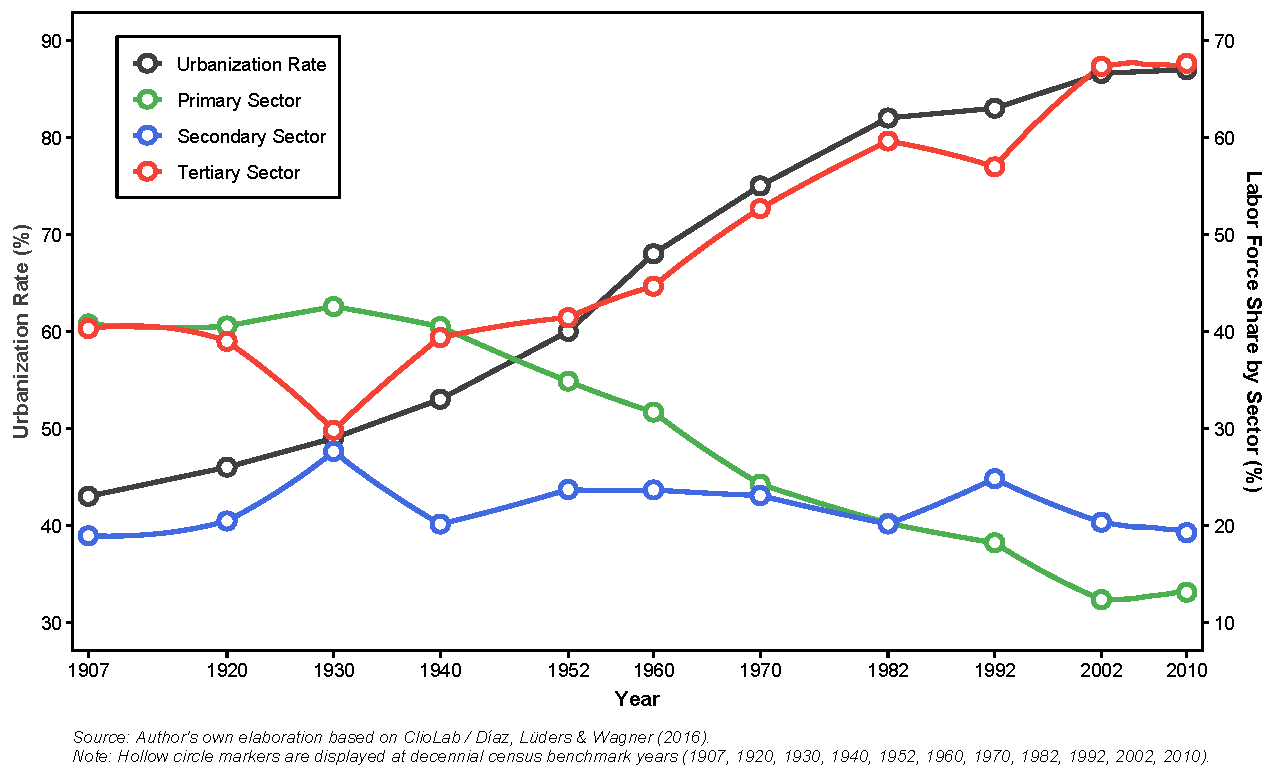
\includegraphics[width=0.90\textwidth]{figures/sec51/fig06_urbanization_labor_sectors.pdf}
\caption{Sectoral labor-force composition and urbanization in Chile, 1907--2010.}
\label{fig:sec51_urban_labor}
\begin{minipage}{0.90\textwidth}\footnotesize
\textit{Source:} Author's elaboration from Clio-Lab PUC historical statistics \citep{DiazLudersWagner2016}. Sectoral series refer to the labor force; urbanization refers to population. These measures have different denominators. Census urbanization observations are plotted as points.
\end{minipage}
\end{figure}

\paragraph{Wave I: Selective incorporation and coercive backlash, 1932--1947.}
The first wave emerged during the reconstruction of the 1930s and reached its crest in the mid-1940s. The 1931 Labor Code established a national framework for collective organization, but incorporation was highly uneven. Urban unions gained a recognized place in industrial relations and electoral politics, while agricultural workers remained subject to estate-level authority and legal restrictions \citep{Milos2008,Loveman1976}. The developmental state expanded productive and social capacities while preserving a differentiated labor regime between city and countryside.

This tension was visible from the beginning. The collapse of the export economy produced unemployment on a scale that weakened labor's immediate bargaining position, but it also destabilized established relations of authority. Rural workers and \emph{inquilinos} used petitions, strikes, and clandestine organization to demand statutory wages, written contracts, and security of tenure. The Ranquil conflict of 1934 exposed the coercive limits of incorporation in the countryside. Under the Popular Front, Communist and Socialist organizers intensified efforts to organize rural labor even as coalition governments remained cautious about confronting landowners directly \citep{Loveman1976}.

By the mid-1940s, rural mobilization converged with renewed industrial militancy. The Plaza Bulnes massacre and the general strikes of January and February 1946 marked the urban-industrial crest of this wave \citep{BravoVargas2017}. Registered agricultural petitions also rose sharply and reached their maximum in 1947 in the series assembled from Loveman's archival evidence (Figure~\ref{fig:sec51_petitions}). This is one reason the 1943--1947 profitability window in Table~\ref{tab:profitability_decomposition} should not be mistaken for the beginning of the wave: it captures the final observed segment of a conflict that had been building since the 1930s.

Distributional accounts are consistent with this tightening conflict. During 1943--1947, a declining profit share ($-5.53$ percent per annum) accounted for the primary negative contribution to profit-rate growth in the chapter's decomposition (Table~\ref{tab:profitability_decomposition}). While this pattern demonstrates that workers were gaining distributional ground in the observed interval, it reflects rather than explains the underlying political mobilization.

The state responded through legal segmentation and political repression. Law 8,811, enacted in July 1947, recognized agricultural unions while confining them to individual \emph{fundos}, restricting the seasonal timing of petitions, and imposing eligibility rules that blocked organization across estates \citep{Chile1947}. The following year, Law 8,987 outlawed the Communist Party and excluded targeted militants from electoral and union activity \citep{Chile1948}. These measures did not resolve rural grievances; they suppressed the organizational channels through which those grievances had been articulated.

The closure of rural organization altered the geography of conflict. Migration to urban centers was driven by structural factors predating the late 1940s repression, but the combination of agrarian stagnation, restricted rural organization, urban industrial concentration, and expanding municipal services made cities central to popular politics.

\begin{figure}[htbp]
\centering
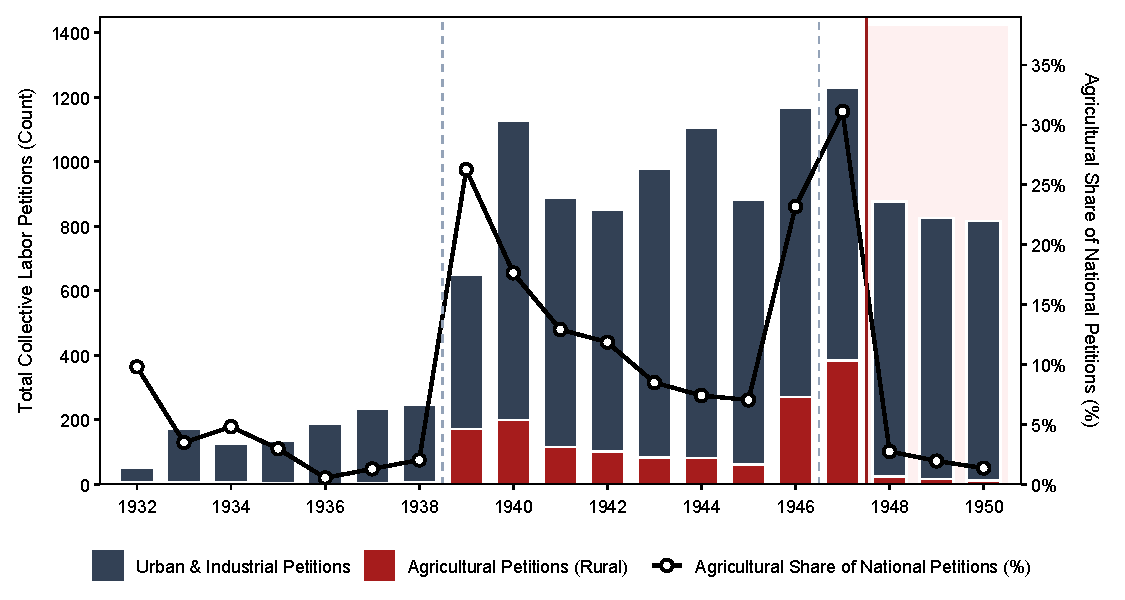
\includegraphics[width=0.88\textwidth]{figures/sec51/fig00_labor_petitions_composition_1932_1950.pdf}
\caption{Recorded collective labor petitions by sector, 1932--1950.}
\label{fig:sec51_petitions}
\begin{minipage}{0.88\textwidth}\footnotesize
\textit{Source:} Author's archival compilation from \citet{Loveman1976}. Petitions measure registered collective demands under the prevailing legal framework, not all forms of social conflict.
\end{minipage}
\end{figure}

\paragraph{Wave II: Coercive containment and urban recomposition, 1948--1958.}
The second wave was defined less by the disappearance of conflict than by its containment and relocation. The restrictions introduced in 1947--1948 narrowed legal space for rural and left organization. During the Ib\'a\~nez administration, the stabilization programme associated with the Klein--Saks mission added statutory wage restraint, credit contraction, and price increases on public transport and foodstuffs. Real wages fell sharply in the mid-1950s while inflation accelerated, shifting the costs of stabilization onto wage earners through workplace discipline and household consumption.

The profitability decomposition documents the distributional consequences of this containment. Between 1948 and 1958, a rising profit share ($+3.11$ percent per annum) provided the largest positive contribution to profit-rate growth ($+2.93$ percent per annum, Table~\ref{tab:profitability_decomposition}), while capital deepening ($-2.60$ log points) offset gains in potential labor productivity ($+2.29$ log points). Distribution shifted toward capital even as industrial and urban transformation continued.

Urban society, however, became more difficult to contain. Industrialization and public investment drew migrants toward the cities without providing factory employment or adequate housing on a commensurate scale. Rather than forming an inert residual of incomplete industrialization, urban neighborhoods became autonomous centers of collective action where migrants, factory workers, informal wage earners, and women organized around transport tariffs, food prices, housing, clinics, and municipal utilities.

In April 1957, protests over transit fare hikes erupted into a nationwide urban revolt, met by military suppression in Santiago, Valpara\'{\i}so, and Concepci\'on. In October 1957, organized families occupied land south of Santiago to establish the \emph{poblaci\'on} La Victoria. Pobladores did not merely petition the state for housing; they occupied land, organized settlement committees, constructed basic infrastructure, and negotiated collectively with public authorities \citep{Garces2002,Murphy2015}. While social conflict is sometimes characterized as having simply shifted from countryside to city, rural grievances persisted alongside industrial unionism and an emerging pobladores movement. What changed was the density of organizational ties linking these arenas.

\paragraph{Wave III: The Long Sixties and the rise of the Unidad Popular, 1959--1970.}
The Long Sixties transformed that urban and rural recomposition into a broader cycle of mobilization. Industrial workers expanded their demands beyond wages toward workplace control, challenging managerial authority over production quotas, safety, and the labor process. Inter-industry solidarity deepened through major conflicts, including the support of Huachipato steelworkers for the 1960 Lota coal strike, while state violence, such as the 1966 killings at the El Salvador copper mine, radicalized union federations \citep{Thielemann2018}.

In the countryside, the Agrarian Reform Law (Law 16,640) and the Rural Unionization Law (Law 16,625) enacted in 1967 dismantled the estate-bound restrictions of Law 8,811, recognizing communal unions and provincial confederations \citep{Chile1967}. Agricultural union membership expanded from 1,658 workers across 24 unions in 1964 to 127,680 members across 488 unions by mid-1970 \citep{DeVylder1976}. Across the economy as a whole, national union density over employed workers doubled from 11.2 percent in 1964 to 22.9 percent by 1970 \citep{OsorioPolanco2021} (Figure~\ref{fig:sec51_wageshare_unionization}). The organizational infrastructure of labor had become dense enough to coordinate action across sectors and regions.

Simultaneously, \emph{pobladores} expanded the politics of social reproduction beyond the wage relation. Land occupations, neighborhood committees, and demands for clinics, schools, transport, water, and paved roads turned access to the city into a field of collective bargaining with the state \citep{Garces2002,Murphy2015}. In centers such as Concepci\'on, industrial unions, student federations, and neighborhood assemblies coordinated strike support and shared logistical resources \citep{Schlotterbeck2018}. The popular movement supporting the Unidad Popular was an articulation of differentiated organized constituencies forged through the uneven development of the period.

Distributional mobilization unfolded within an expanding rather than a contracting economy: across the 1959--1970 accounting interval, the profit rate rose from 8.16 percent to 12.23 percent, supported by positive contributions from the profit share, capacity utilization, and potential labor productivity (Table~\ref{tab:profitability_decomposition}). Sustained accumulation, a larger urban labor force, and denser institutional networks expanded workers' capacity to press claims on national income, property, and state policy.

While a Kaleckian political mechanism links sustained high employment to weakened labor discipline, Chile had not attained generalized full employment. The sectoral and institutional dynamic was decisive: tighter conditions in unionized industries and rising national union density bolstered workers' collective bargaining power even while an informal reserve army persisted in peripheral services.

\begin{figure}[htbp]
\centering
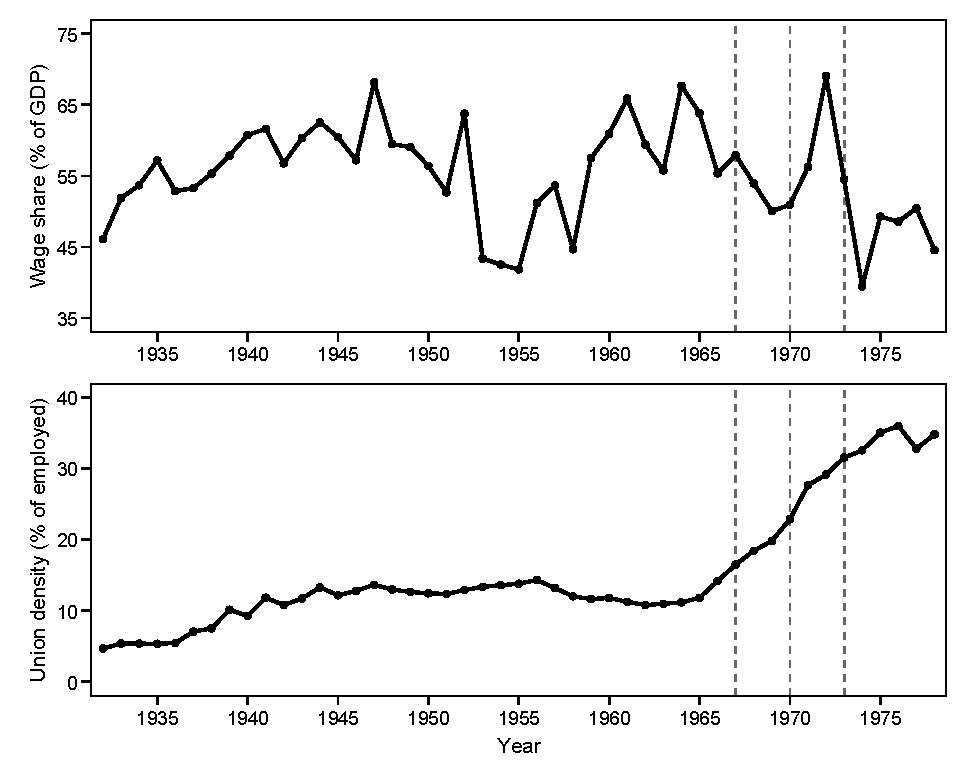
\includegraphics[width=0.88\textwidth]{figures/sec51/fig07_wageshare_unionization.pdf}
\caption{Wage share and unionization in Chile, 1932--1978.}
\label{fig:sec51_wageshare_unionization}
\begin{minipage}{0.88\textwidth}\footnotesize
\textit{Source:} Author's elaboration from \citet{Astorga2023} for Panel~A and \citet{OsorioPolanco2021} for Panel~B. Panel~A reports the functional wage share ($W/Y$, percent of GDP). Panel~B reports union density over employed workers. Vertical dashed lines mark the 1967 agrarian reform and rural unionization statutes (Laws 16,640 and 16,625), the September 1970 election of Salvador Allende, and the September 11, 1973 military coup.
\end{minipage}
\end{figure}

\paragraph{Wave IV: The UP administration and the crisis of accumulation, 1970--1973.}
Allende's election in September 1970 linked these popular movements directly with executive power. The UP programme connected income redistribution to the nationalization of strategic mineral resources, expansion of the social property area, agrarian expropriation, and structural planning. Yet the organizations forged during the preceding waves did not become passive extensions of government. Factory requisitions, land occupations, and community distribution networks frequently pushed ahead of the executive's statutory timetable \citep{Winn1986,Winn2016,Schlotterbeck2018}, generating dynamic tension between state policy and autonomous popular mobilization.

The administration's first year produced an exceptionally large distributive expansion. Real employee remuneration rose by 54.9 percent in 1971 following statutory wage adjustments \citep{DeVylder1976}, and the wage share rose from 50.9 percent of GDP in 1970 to 69.0 percent in 1972 \citep{Astorga2023}. The growth-accounting decomposition reveals a severe initial profit squeeze: the profit rate fell from 12.23 percent in 1970 to 6.57 percent in 1972, while the net accumulation rate declined from 4.23 to 1.85 percent and gross accumulation from 11.63 to 7.64 percent (Table~\ref{tab:accumulation_accounting}). The profit share accounted for most of this decline between 1971 and 1972 (Table~\ref{tab:profitability_decomposition}, Panel~B).

That initial distributive squeeze cannot be projected mechanically over the full three-year interval. Across 1971--1973, relative capital prices ($-4.35$ percent) and capacity utilization ($-4.78$ percent) provided the dominant negative contributions to profit-rate growth, while the contribution of the profit share changed sign (+1.94 percent, Table~\ref{tab:profitability_decomposition}, Panel~A). The annual accounts for 1973 make this divergence evident: the measured profit rate rebounded from 6.57 percent in 1972 to 9.12 percent in 1973, yet net capital accumulation slowed further to 1.71 percent (Table~\ref{tab:accumulation_accounting}). Because annual 1973 data aggregate the final eight months of the UP with the first four months of military dictatorship, they cannot separate pre-coup strikes from post-coup wage repression. They nevertheless demonstrate that profitability alone cannot explain the collapse of capital accumulation.

The terminal crisis concentrated contradictions that had accumulated across multiple decades: an industrial base dependent on imported capital goods and foreign finance; agrarian stagnation that generated wage-good bottlenecks; incomplete urban labor absorption; and a densely organized popular movement capable of mounting structural challenges to property and state authority.

The Unidad Popular concentrated rather than initiated these contradictions. Its redistributive programme accelerated popular mobilization within external and productive boundaries inherited from the developmental era. The next section examines the balance-of-payments constraints and monthly macroeconomic dynamics that governed the subsequent crisis.

\begin{table}[H]
	\centering
	\footnotesize
	\setlength{\tabcolsep}{3.8pt}
	\caption{Social Conflict Waves and Profitability Decomposition, Chile, 1943--1975}
	\label{tab:profitability_decomposition}
	
	\vspace{0.2em}

	
	\begin{tabular}{L{3.5cm}C{1.75cm}C{1.75cm}C{1.75cm}C{1.75cm}C{1.75cm}C{1.75cm}}
		\toprule
		\textbf{Wave of Social Conflict} 
		& \textbf{Profit Rate} 
		& \textbf{Profit Sh.} 
		& \textbf{Rel.\ Price} 
		& \textbf{Cap.\ Util.} 
		& \textbf{Lab.\ Prod.} 
		& \textbf{Cap.\ Deep.} \\
		
		& \small{$\Delta\ln r$} 
		& \small{$\Delta\ln(1-\omega)$} 
		& \scriptsize{$\Delta\ln(P_Y/P_K)$} 
		& \small{$\Delta\ln\mu$} 
		& \small{$\Delta\ln y^p$} 
		& \small{$-\Delta\ln k$} \\
		\midrule
		% Block 1: Regime Averages
		\multicolumn{7}{l}{\underline{\textit{A. Social Conflict Waves (Annualized Rates and \% Shares)}}} \\[0.3em]
		
		Wave I: Observed accounting segment (1943--1947)
		& \makecell[c]{-2.84\% \\ }
		& \makecell[c]{-5.53\% \\ (+194.9\%)}
		& \makecell[c]{+2.63\% \\ (-92.7\%)}
		& \makecell[c]{+0.62\% \\ (-21.7\%)}
		& \makecell[c]{-0.21\% \\ (+7.6\%)}
		& \makecell[c]{-0.34\% \\ (+11.9\%)} \\[0.5em]
		
		Wave II: Containment and urban recomposition (1948--1958)
		& \makecell[c]{+2.93\% \\ }
		& \makecell[c]{+3.11\% \\ (+106.1\%)}
		& \makecell[c]{-0.10\% \\ (-3.3\%)}
		& \makecell[c]{+0.23\% \\ (+7.9\%)}
		& \makecell[c]{+2.29\% \\ (+77.9\%)}
		& \makecell[c]{-2.60\% \\ (-88.6\%)} \\[0.5em]
		
		Wave III: Long Sixties accounting interval (1959--1970)
		& \makecell[c]{+2.07\% \\ }
		& \makecell[c]{+1.31\% \\ (+63.3\%)}
		& \makecell[c]{+0.45\% \\ (+21.6\%)}
		& \makecell[c]{+0.97\% \\ (+46.9\%)}
		& \makecell[c]{+1.72\% \\ (+83.0\%)}
		& \makecell[c]{-2.38\% \\ (-114.8\%)} \\[0.5em]
		
		Wave IV: UP crisis accounting interval (1971--1973)
		& \makecell[c]{-7.65\%\\  }
		& \makecell[c]{+1.94\% \\ (-25.3\%)}
		& \makecell[c]{-4.35\% \\ (+56.9\%)}
		& \makecell[c]{-4.78\% \\ (+62.5\%)}
		& \makecell[c]{-1.23\% \\ (+16.0\%)}
		& \makecell[c]{+0.77\% \\ (-10.1\%)} \\[0.8em]
		
		\midrule
		
		% Block 2: Annual Crisis Cycle
		\multicolumn{7}{l}{\underline{\textit{B. Terminal Crisis Cycle: Annual Log Changes and \% Shares}}} \\[0.3em]
		
		$1970 \to 1971$: Reactivation peak 
		& \makecell[c]{-14.05\% \\ }
		& \makecell[c]{-11.44\% \\  (+81.4\%)}
		& \makecell[c]{-7.90\% \\ (+56.2\%)}
		& \makecell[c]{+5.92\% \\ (-42.1\%)}
		& \makecell[c]{-0.43\% \\ (+3.1\%)}
		& \makecell[c]{-0.20\% \\ (+1.4\%)} \\[0.5em]
		
		$1971 \to 1972$: Profit squeeze 
		& \makecell[c]{-48.08\% \\ }
 		& \makecell[c]{-34.60\% \\ (+72.0\%)}
		& \makecell[c]{-10.42\% \\ (+21.7\%)}
		& \makecell[c]{-2.52\% \\ (+5.2\%)}
		& \makecell[c]{-2.27\% \\ (+4.7\%)}
		& \makecell[c]{+1.74\% \\ (-3.6\%)} \\[0.5em]
		
		$1972 \to 1973$: Annual observation spanning the coup 
		& \makecell[c]{+32.78\% \\ }
		& \makecell[c]{+38.48\% \\ (+117.4\%)}
		& \makecell[c]{+1.72\% \\ (+5.3\%)}
		& \makecell[c]{-7.04\% \\ (-21.5\%)}
		& \makecell[c]{-0.18\% \\ (-0.5\%)}
		& \makecell[c]{-0.20\% \\ (-0.6\%)} \\[0.5em]
		
		$1973 \to 1974$: DL 522 compression 
		& \makecell[c]{+15.74\%}
		& \makecell[c]{+28.59\% \\ {\scriptsize (+181.7\%)}}
		& \makecell[c]{-11.47\% \\ {\scriptsize (-72.9\%)}}
		& \makecell[c]{-0.72\% \\ {\scriptsize (-4.6\%)}}
		& \makecell[c]{+4.04\% \\ {\scriptsize (+25.7\%)}}
		& \makecell[c]{-4.70\% \\ {\scriptsize (-29.9\%)}} \\[0.5em]
		
		$1974 \to 1975$: Chicago shock therapy 
		& \makecell[c]{-48.97\%}
		& \makecell[c]{-17.70\% \\  (+36.2\%)}
		& \makecell[c]{-16.24\% \\ (+33.2\%)}
		& \makecell[c]{-14.78\% \\ (+30.2\%)}
		& \makecell[c]{+8.97\% \\ (-18.3\%)}
		& \makecell[c]{-9.22\% \\ (+18.8\%)} \\
		\bottomrule
	\end{tabular}%
	
	\vspace{0.5em}
	
	\begin{minipage}{\textwidth}
		\scriptsize
		\textit{Notes.} Growth-accounting decomposition using the identity $\Delta \ln r_t \equiv \Delta \ln(1-\omega_t) + \Delta \ln(P_{Y,t}/P_{K,t}) + \Delta \ln \mu_t + \Delta \ln y^p_t - \Delta \ln k_t$. Values outside parentheses are annualized log contributions (\% p.a.). Values inside parentheses report the component's share of the total change, computed as $(\Delta \ln X_i / \Delta \ln r_t) \times 100\%$. A positive share indicates the component moved in the same direction as the total change; a negative share indicates it offset the total change. Shares may exceed 100\% due to normalization by the net total change. Source: Author's own elaboration (Chapter 2).
	\end{minipage}
\end{table}

\begin{table}[H]
	\centering
	\footnotesize % Matched to Table 1
	\setlength{\tabcolsep}{4pt}
	
	\caption{Capital Accumulation Response Across the Terminal Crisis Cycle, Chile, 1964--1975}
	\label{tab:accumulation_accounting}
	
	\vspace{0.2em}
	
	% Reuse the custom column types defined in Table 1's preamble 
	% OR define them here if they are local. 
	% Assuming L{} and C{} are already defined globally in your preamble:
	
	% Total Width Calculation to match Table 1:
	% Table 1: 3.5 + (6 * 1.75) = 3.5 + 10.5 = 14.0 cm
	% Table 2: 3.5 + (5 * X) = 14.0 => 5X = 10.5 => X = 2.1 cm
	% So we use C{2.1cm} for the numeric columns.
	
	\begin{tabular}{L{3.5cm} C{2.1cm} C{2.1cm} C{2.1cm} C{2.1cm} C{2.1cm}}
		\toprule
		\textbf{Episode / Year} 
		& \textbf{Profit Rate} 
		& \textbf{Accum.\ Ratio} 
		& \textbf{Gross Acc.\ Rate} 
		& \textbf{Depreciation Rate} 
		& \textbf{Net Acc.\ Rate} \\
		
		& $\boldsymbol{r}$ (\%) 
		& $\boldsymbol{\chi}$ (ratio) 
		& $g^{\mathrm{gross}}_K$ (\%) 
		& $\boldsymbol{\delta}$ (\%) 
		& $g^n_K$ (\%) \\
		\midrule
		
		\multicolumn{6}{l}{\underline{\textit{A. Christian Democratic Administration (1964--1970)}}} \\[0.3em]
		
		1964 (Baseline)       & 8.16  & 1.530 & 12.49 & 7.67 & 4.82 \\[0.2em]
		1965                  & 8.59  & 1.244 & 10.69 & 6.94 & 3.75 \\[0.2em]
		1966                  & 10.94 & 0.972 & 10.63 & 6.97 & 3.66 \\[0.2em]
		1967                  & 10.14 & 1.066 & 10.81 & 7.06 & 3.75 \\[0.2em]
		1968                  & 11.29 & 0.991 & 11.20 & 7.24 & 3.96 \\[0.2em]
		1969 (Peak Profit.)   & 12.79 & 0.857 & 10.96 & 7.14 & 3.82 \\[0.2em]
		1970 (Inherited)      & 12.23 & 0.951 & 11.63 & 7.40 & 4.23 \\[0.5em]
		
		\midrule
		
		\multicolumn{6}{l}{\underline{\textit{B. Unidad Popular Administration (1971--1973)}}} \\[0.3em]
		
		1971 (Reactivation)   & 10.62 & 0.953 & 10.12 & 6.78 & 3.34 \\[0.2em]
		1972 (Squeeze)        & 6.57  & 1.162 & 7.64  & 5.78 & 1.85 \\[0.2em]
		1973 (Coup year)      & 9.12  & 0.821 & 7.48  & 5.78 & 1.71 \\[0.5em]
		
		\midrule
		
		\multicolumn{6}{l}{\underline{\textit{C. Military Dictatorship \& Shock Therapy (1974--1975)}}} \\[0.3em]
		
		1974 (Compression)    & 10.67 & 0.811 & 8.65  & 6.27 & 2.38 \\[0.2em]
		1975 (Collapse)       & 6.54  & 1.035 & 6.77  & 5.56 & 1.21 \\
		
		\bottomrule
	\end{tabular}%
	
	\vspace{0.5em}
	
	\begin{minipage}{\textwidth}
		\scriptsize
		\textit{Notes.} Accumulation accounting for fixed capital assets ($K_t \equiv K_{\mathrm{ME},t} + K_{\mathrm{NRC},t}$), excluding residential construction. Gross accumulation is $g^{\mathrm{gross}}_{K,t} \equiv I^{\mathrm{gross}}_t/K_{t-1}$; physical depreciation is $\delta_t \equiv D_t/K_{t-1}$; net accumulation is $g^n_{K,t} \equiv I^{\mathrm{net}}_t/K_{t-1}$; and the gross investment-to-surplus ratio (accumulation ratio) is $\chi_t \equiv g^{\mathrm{gross}}_{K,t}/r_t$. All observations satisfy the exact identity $g^n_{K,t} \equiv \chi_t r_t - \delta_t$, subject to displayed rounding. The profit rate is a level, not its growth rate. Annual 1973 observations span the coup. Source: Author's own elaboration (Chapter 2).
	\end{minipage}
\end{table}




\subsection{Stylized Facts of Peripheral Accumulation, Distribution, and External Constraints}
\label{sec:stylized_facts}
% ==============================================================================
% SECTION 5.2: STYLIZED FACTS OF PERIPHERAL ACCUMULATION, DISTRIBUTION, AND EXTERNAL CONSTRAINTS
% ==============================================================================

\subsubsection{Structural Constraints of Peripheral Transition: An Accounting Anchor}
\label{sec:stylized_material_bounds}

The political mobilization and redistributive policies analyzed in Section~\ref{sec:historical_background} unfolded within external material constraints. The Chilean economy relied on imported machinery, intermediate spare parts, and foreign trade credits to sustain domestic employment and basic wage-goods production. Mainstream accounts \citep{DornbuschEdwards1990,Edwards2024} attribute the subsequent macroeconomic crisis to fiscal deficits and unconstrained money creation that depleted reserves and triggered inflation. In contrast, structuralist and dependency traditions \citep{Stallings1978,DeVylder1976} emphasize balance-of-payments vulnerability, intermediate import dependency, and external credit restrictions. Comparing these perspectives requires establishing the descriptive sequence between external balance-sheet deterioration, domestic inflation, and monetary expansion.

In a subordinate open economy without reserve-currency status, convertible international reserves constrain the ability of the central bank to settle external obligations, finance intermediate imports, and maintain exchange parity. To track this external balance-sheet position, I define the Central Bank Solvency Ratio relative to Base Money:
\begin{equation}
    \text{SolvR}^{H}_t \equiv \frac{e_t \cdot IR_t}{H_t \cdot 1000},
    \label{eq:solvency_ratio_base_def}
\end{equation}
where $e_t$ is the official exchange rate (standardized in pesos per USD in the Central Bank database), $IR_t$ represents gross international reserves in USD millions from the IMF (yielding a numerator $e_t \cdot IR_t$ in millions of pesos), and $H_t$ denotes domestic base money liabilities recorded in thousands of millions of pesos (billions, \emph{miles de millones de pesos}), scaled by $1{,}000$ to express liabilities in millions of pesos and ensure dimensional consistency. As foreign reserves fell and external credit lines contracted, reserve coverage of the domestic monetary base declined. The descriptive sequence therefore raises the empirical question of whether domestic money growth preceded inflation as an autonomous driver or responded to emerging external bottlenecks and domestic cost pressures.

\subsubsection{Long-Span Balance of Payments Accounting: Reserve Accumulation and the 1971 Capital-Flow Reversal (1958--1975)}
\label{sec:stylized_bop_accounting}

In standard national accounting, the annual change in official Central Bank international reserves ($\Delta IR_t$) satisfies the identity:
\begin{equation}
    \Delta IR_t \equiv CA_t + KA_t + EO_t + SDR_t
    \label{eq:bop_reserves_identity}
\end{equation}
where $CA_t$ is the current account balance, $KA_t$ denotes net capital inflows, $EO_t$ represents net errors and omissions, and $SDR_t$ denotes allocations of IMF Special Drawing Rights. Net errors and omissions represent an accounting residual that, in peripheral contexts confronting trade and exchange controls, is consistent with unrecorded capital flight and trade misinvoicing \citep{Stallings1978}. Two distinct reserve concepts must be separated throughout this analysis: gross international reserves ($IR_t$), which record total foreign exchange assets held by the monetary authority, and net international reserves ($IR^{\text{net}}_t$), which subtract short-term foreign liabilities from gross holdings.

\begin{landscape}
\begin{table}[!htbp]
\centering
\scriptsize
\caption{Long-Span Balance of Payments Accounting and International Reserves Dynamics (Chile, 1958--1975): Official BCCh Cash Flows vs. WBOP Global Accrual Accounts}
\label{tab:bop_reserves_accounting}
\renewcommand{\arraystretch}{1.15}
\setlength{\tabcolsep}{3.0pt}
\resizebox{\linewidth}{!}{%
\begin{tabular}{lrrrrrrrrrrrrrrrrrr}
\toprule
& \textbf{Ib\'a\~nez} & \multicolumn{6}{c}{\textbf{Jorge Alessandri (1959--1964)}} & \multicolumn{6}{c}{\textbf{Eduardo Frei Montalva (1965--1970)}} & \multicolumn{3}{c}{\textbf{Unidad Popular (1971--1973)}} & \multicolumn{2}{c}{\textbf{Junta (1974--75)}} \\
\cmidrule(lr){2-2} \cmidrule(lr){3-8} \cmidrule(lr){9-14} \cmidrule(lr){15-17} \cmidrule(lr){18-19}
\textbf{Metric / USD Millions} & \textbf{1958} & \textbf{1959} & \textbf{1960} & \textbf{1961} & \textbf{1962} & \textbf{1963} & \textbf{1964} & \textbf{1965} & \textbf{1966} & \textbf{1967} & \textbf{1968} & \textbf{1969} & \textbf{1970} & \textbf{1971} & \textbf{1972} & \textbf{1973} & \textbf{1974} & \textbf{1975} \\
\midrule
\multicolumn{19}{l}{\textbf{A. Official Cash-Basis Balance of Payments (Central Bank of Chile / Stallings 1978, USD Millions)}} \\[0.2em]
Current Account ($CA$) & --- & $-24.8$ & $-148.1$ & $-241.1$ & $-181.9$ & $-157.8$ & $-131.6$ & $-56.6$ & $-82.2$ & $-127.4$ & $-135.3$ & $-5.6$ & $-102.9$ & \textbf{$-205.5$} & \textbf{$-404.8$} & $-294.6$ & $-210.8$ & $-491.3$ \\
Capital Account ($KA$) & --- & 20.8 & 76.3 & 187.6 & 133.2 & 107.6 & 152.1 & 65.8 & 168.0 & 125.5 & 294.6 & 222.5 & 267.5 & \textbf{$-26.5$} & 327.4 & 242.3 & 228.0 & 298.7 \\
Net Errors \& Omissions ($EO$) & --- & 28.6 & 43.4 & $-55.1$ & $-0.3$ & 22.0 & 2.9 & 37.5 & 33.8 & $-21.5$ & $-41.4$ & $-42.4$ & $-72.9$ & $-84.5$ & \textbf{$-171.6$} & $-60.0$ & $-62.1$ & $-92.4$ \\
SDR Allocations ($SDR$) & 0.0 & 0.0 & 0.0 & 0.0 & 0.0 & 0.0 & 0.0 & 0.0 & 0.0 & 0.0 & 0.0 & 0.0 & 21.8 & 16.7 & 18.2 & 0.0 & 0.0 & 0.0 \\
\midrule
Net Reserve Change ($\Delta IR$) & --- & \textbf{24.6} & \textbf{$-28.4$} & \textbf{$-108.6$} & \textbf{$-49.0$} & \textbf{$-28.2$} & \textbf{23.4} & \textbf{46.7} & \textbf{119.6} & \textbf{$-23.4$} & \textbf{117.9} & \textbf{174.5} & \textbf{113.5} & \textbf{$-299.8$} & \textbf{$-230.8$} & \textbf{$-112.3$} & \textbf{$-44.9$} & \textbf{$-285.0$} \\
Net International Reserves ($IR^{\text{net}}_t$) & 29.6 & 105.4 & 72.8 & $-5.2$ & 15.4 & $-24.3$ & \textbf{$-16.5$} & 35.2 & 77.4 & 54.3 & 125.4 & 285.2 & \textbf{393.5} & 162.7 & \textbf{75.8} & 167.4 & 94.0 & \textbf{$-129.2$} \\
\midrule
\multicolumn{19}{l}{\textbf{B. Capital Account Reversal, External Drainage, and Cumulative Flows}} \\[0.2em]
Net External Drain ($CA+KA+EO$) & --- & $+24.6$ & $-28.4$ & $-108.6$ & $-49.0$ & $-28.2$ & $+23.4$ & $+46.7$ & $+119.6$ & $-23.4$ & $+117.9$ & $+174.5$ & $+91.7$ & \textbf{$-316.5$} & \textbf{$-249.0$} & $-112.3$ & $-44.9$ & $-285.0$ \\
Drain Share of $IR_{t-1}$ & --- & --- & --- & --- & --- & --- & --- & --- & --- & --- & --- & --- & --- & \textbf{80.4\%} & \textbf{153.0\%} & 148.2\% & 26.8\% & 303.2\% \\
Cumulative $\sum KA$ & --- & \multicolumn{6}{c}{$+\$677.6\text{M}$ (Alessandri Total)} & \multicolumn{6}{c}{\textbf{$+\$1,143.9\text{M}$} (Frei Montalva Total)} & \multicolumn{3}{c}{$+\$543.2\text{M}$ (UP Total)} & \multicolumn{2}{c}{$+\$526.7\text{M}$} \\
Cumulative $\sum CA$ & --- & \multicolumn{6}{c}{$-\$885.3\text{M}$ (Alessandri Total)} & \multicolumn{6}{c}{\textbf{$-\$510.0\text{M}$} (Frei Montalva Total)} & \multicolumn{3}{c}{$-\$904.9\text{M}$ (UP Total)} & \multicolumn{2}{c}{$-\$702.1\text{M}$} \\
\midrule
\multicolumn{19}{l}{\textbf{C. Global Accrual Balance of Payments (WBOP, \citealt{NievasPiketty2025})}} \\[0.2em]
WBOP Current Account (USD M) & $-271.8$ & $-189.5$ & $-155.3$ & $-265.4$ & $-194.4$ & $-308.2$ & $-212.8$ & $-103.4$ & $-179.4$ & $-135.9$ & $-70.9$ & $+61.8$ & $-147.7$ & \textbf{$-421.6$} & \textbf{$-550.8$} & $-618.1$ & $-105.5$ & \textbf{$-470.6$} \\
WBOP Current Account (\% GDP) & $-7.74\%$ & $-5.00\%$ & $-3.40\%$ & $-5.19\%$ & $-3.26\%$ & $-5.21\%$ & $-3.37\%$ & $-1.60\%$ & $-2.37\%$ & $-1.82\%$ & $-0.93\%$ & $+0.70\%$ & $-1.53\%$ & \textbf{$-3.64\%$} & \textbf{$-4.40\%$} & $-3.47\%$ & $-0.61\%$ & \textbf{$-5.85\%$} \\
Net Foreign Wealth / IIP (\% GDP)& $-67.0\%$ & $-69.3\%$ & $-61.7\%$ & $-58.1\%$ & $-54.3\%$ & $-57.9\%$ & $-59.2\%$ & $-61.1\%$ & $-53.5\%$ & $-56.7\%$ & $-57.4\%$ & $-50.2\%$ & $-54.6\%$ & $-47.7\%$ & $-49.4\%$ & $-33.6\%$ & $-46.4\%$ & \textbf{$-100.6\%$} \\
\bottomrule
\end{tabular}%
}
\vspace{0.3em}
\begin{minipage}{\linewidth}
\scriptsize
\textbf{Sources and Notes:} Official cash-basis Balance of Payments flows (1960--1975), Net Errors and Omissions, and SDR allocations sourced from the Banco Central de Chile (BCCh) REST API and Base de Datos Estad\'{\i}sticos (BDE), complemented by historical balance-of-payments ledgers. 1958--1959 cash entries sourced directly from \citet[Table~7.4, p.~178]{Stallings1978}, citing contemporary BCCh records. Net international reserves ($IR^{\text{net}}_t$) record liquid foreign exchange assets net of short-term central bank foreign liabilities, compiled from BCCh historical ledgers and \citet{Stallings1978}, accounting for negative net balances during the 1961--1964 exchange crises and 1975; gross foreign reserve assets from IMF International Financial Statistics remain positive in all years. Global accrual balance of payments series and Net International Investment Position (NIIP) sourced from the World Historical Balance of Payments Database \citep{NievasPiketty2025}. The balance-of-payments reserves identity holds exactly: $\Delta IR_t \equiv CA_t + KA_t + EO_t + SDR_t$. Discrepancies between cash and accrual accounts reflect distinct institutional accounting conventions: cash ledgers record physical foreign exchange settlements at the Central Bank window, whereas WBOP accrual accounts adhere to modern BPM6 standards, incorporating legally accrued but unpaid debt service (under the November 1971 debt moratorium), reinvested foreign mining profits, and global bilateral trade partner reconciliations. Both records confirm that in 1971, net external financing experienced a sharp contraction of $-\$294.0$ million ($KA = -\$26.5\text{M}$ vs. $+\$267.5\text{M}$ in 1970), equivalent in magnitude to $98.1\%$ of the calendar-year reserve drain ($\Delta IR = -\$299.8\text{M}$) before domestic fiscal emission accelerated in late 1972.
\end{minipage}
\end{table}
\end{landscape}


Table~\ref{tab:bop_reserves_accounting} reports the balance-of-payments ledger across eighteen years (1958--1975), spanning four developmental regimes in dialogue with \citet{Stallings1978} and the World Historical Balance of Payments database \citep{NievasPiketty2025}. The table presents both cash-basis and accrual-basis accounts. The official BCCh cash ledger \citep[Table~7.4, p.~178]{Stallings1978} records foreign currency settlements that crossed the Central Bank counter, capturing the liquid resources available to defend exchange parity and pay for imports. In contrast, the WBOP database \citep{NievasPiketty2025} reconstructs accounts under modern IMF BPM6 accrual standards, recording primary income debits and interest obligations as they legally accrued, including during the November 1971 debt moratorium.

The pre-1970 administrations established the external balance-sheet position inherited by the Unidad Popular. Under Jorge Alessandri (1958--1964), import liberalization and a fixed nominal exchange rate led to cumulative current account deficits of $-\$885.3$ million. By late 1961, liquid reserves were exhausted, forcing emergency import controls and an eventual currency float in October 1962 that generated an inflation spike; net reserves ended at $-\$16.5$ million in 1964. The Eduardo Frei Montalva administration (1964--1970) instituted a crawling peg and accumulated reserves through external borrowing supported by the Alliance for Progress \citep{FfrenchDavis1973}. Cumulative net foreign capital inflows across Frei's term totaled $+\$1,143.9$ million, while the cumulative sum of annual reserve changes was $+\$548.8$ million. Net capital inflows thus exceeded cumulative reserve accumulation by more than two to one ($208.4\%$), as net reserves rose from $-\$16.5$ million in 1964 to $\$393.5$ million at year-end 1970 (a net stock increase of $+\$410.0$ million; the difference from cumulative annual flows reflects valuation adjustments on non-dollar holdings and the netting of short-term foreign liabilities in the stock measure). The reserve buffer inherited by the UP was therefore anchored in foreign credit lines.

Following the constitutional nationalization of large-scale copper mining on July 11, 1971 (Law 17,450), external financing contracted sharply. Net capital inflows fell from $+\$267.5$ million in 1970 to $-\$26.5$ million in 1971 ($-\$49.9$ million in Stallings' autonomous capital series). In the audited 1958--1975 ledger, 1971 was the only calendar year with negative net capital inflows. This $-\$294.0$ million turnaround in the capital account was equivalent in magnitude to $98.1\%$ of the calendar-year reserve drain ($\Delta IR = -\$299.8$ million), reducing Central Bank liquidity before domestic price acceleration took hold in late 1972.

The reduction in external financing materialized through specific commercial channels. As documented by \citet{DeVylder1976} and \citet{PetrasMorley1975}, international commercial banks curtailed short-term trade credits to Chile from $\$220$ million to $\$35$ million, while the U.S. Export-Import Bank suspended project lending. Foreign suppliers increasingly required cash-in-advance confirmed letters of credit for food and fuel shipments, and replacement parts for imported mining machinery faced delays in foreign ports \citep{Stallings1978}. Net Errors and Omissions recorded negative residuals totaling $-\$389.0$ million across the UP triennium ($-\$72.9$M in 1970, $-\$84.5$M in 1971, and $-\$171.6$M in 1972). Following the September 4, 1970 election, the Santiago stock exchange declined by $48.6\%$ and commercial bank deposits contracted \citep{GirardiBowles2018}. The timing is consistent with capital flight and private asset liquidation beginning prior to the presidential inauguration. While the cash ledger shows positive capital inflows in 1972 ($+\$327.4$M), this reflected the capitalization of debt service following the November 1971 moratorium. On an accrual basis, the WBOP current account deficit widened to $-\$550.8$ million ($-4.40\%$ of GDP) in 1972 and $-\$618.1$ million ($-3.47\%$ of GDP) in 1973, while Central Bank net foreign reserves fell to $\$75.8$ million at year-end 1972.

Following the September 1973 coup, external commercial credits resumed ($KA = +\$228.0$M in 1974 and $+\$298.7$M in 1975), and bilateral debts were rescheduled through the Paris Club. When world copper prices fell in 1975, domestic expenditure compression reduced import volumes. External vulnerability remained visible in the 1975 accounts: the accrual current account deficit reached $-\$470.6$ million ($-5.85\%$ of GDP), net international reserves fell to $-\$129.2$ million, and manufacturing output contracted.

\subsubsection{Terms of Trade, Capacity to Import, and Real Structural Imbalance (1960--1980)}
\label{sec:stylized_terms_of_trade}

To evaluate external purchasing power and physical trade flows, Figures~\ref{fig:solvency_reserves}, \ref{fig:copper_gold}, and \ref{fig:import_capacity} trace the monthly trajectories of foreign reserves, commodity prices, and import capacity across 1960--1980 ($N=252$ continuous calendar months, yielding $N=250$ observations in the transformed econometric sample).

\begin{figure}[!htbp]
\centering
\caption{Central Bank Solvency Ratio ($\text{SolvR}^H$) and Gross International Reserves (1960--1980)}
\label{fig:solvency_reserves}
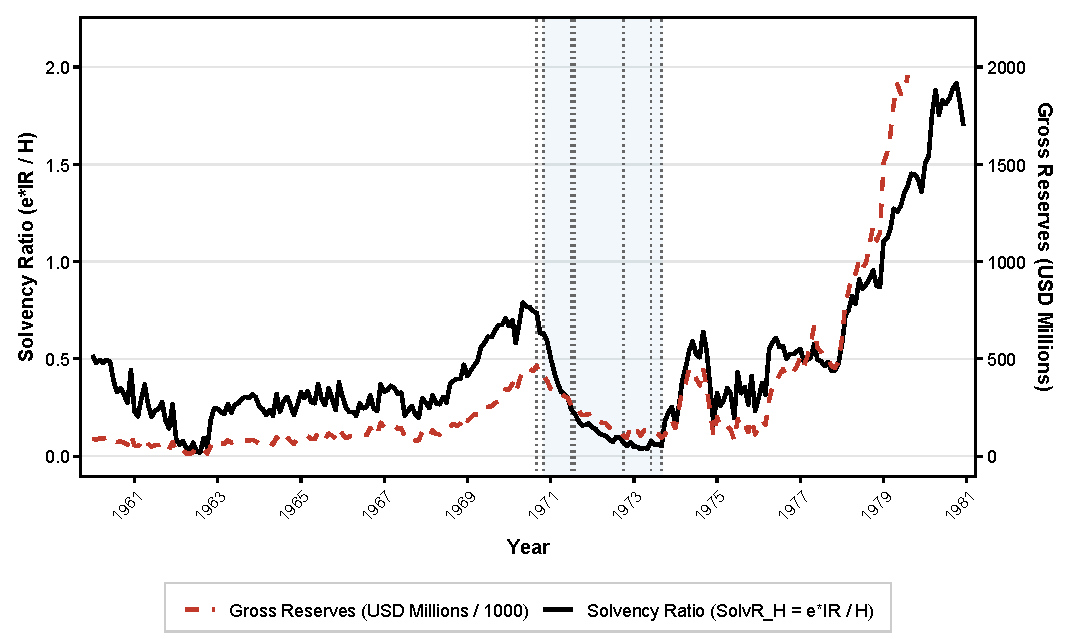
\includegraphics[width=0.88\textwidth]{figures/fig01a_solvency_reserves.pdf}
\begin{minipage}{0.95\textwidth}
\vspace{0.2cm}
\footnotesize
\textbf{Notes:} Monthly series tracking the Central Bank Solvency Ratio relative to Base Money ($\text{SolvR}^{H}_t \equiv \frac{e_t \cdot IR_t}{H_t \cdot 1000}$, left axis, solid black line) and IMF gross international reserves ($IR_t$ in USD millions, right axis, dashed red line). Base money ($H_t$) represents the Central Bank's direct domestic liability base from the archival ledger. Benchmark markers $\mathrm{I}$--$\mathrm{VII}$ defined in Table~\ref{tab:critical_junctures}. Shaded blue region designates the Unidad Popular government (November 1970 -- September 1973). Sourced from Central Bank of Chile REST API and IMF International Financial Statistics.
\end{minipage}
\end{figure}

\begin{figure}[!htbp]
\centering
\caption{World Copper Price and London Gold Price (1960--1980)}
\label{fig:copper_gold}
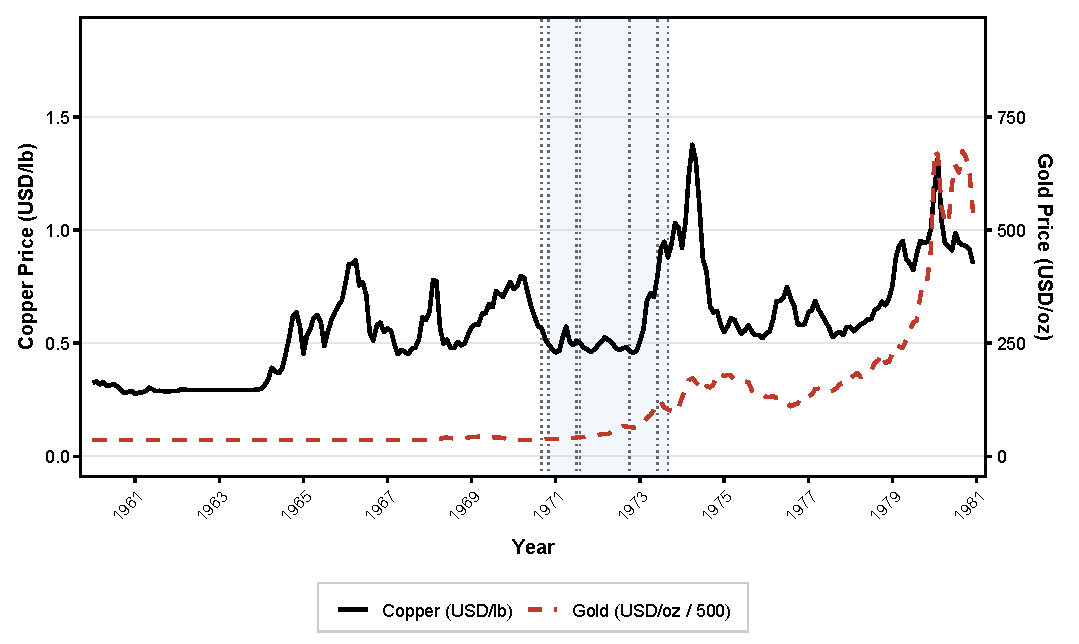
\includegraphics[width=0.88\textwidth]{figures/fig01b_copper_gold.pdf}
\begin{minipage}{0.95\textwidth}
\vspace{0.2cm}
\footnotesize
\textbf{Notes:} Monthly series tracking the London Metal Exchange copper cash price ($P^{\text{Cu}}$ in USD/lb, left axis, solid black line) and London Bullion Market Association gold price ($P^{\text{Gold}}$ in USD/oz / 500, right axis, dashed red line). Benchmark markers $\mathrm{I}$--$\mathrm{VII}$ defined in Table~\ref{tab:critical_junctures}. Shaded blue region designates the Unidad Popular government (November 1970 -- September 1973). Sourced from LME and LBMA via Central Bank of Chile REST API.
\end{minipage}
\end{figure}

The international terms of trade shifted unfavorably during the administration's first year (Figure~\ref{fig:copper_gold}). World copper export prices fell by $25\%$ during 1971, averaging $\$0.47$/lb compared to $\$0.64$/lb across 1969--1970, reducing export revenue during the initial domestic reactivation. Concurrently, the international monetary system absorbed the breakdown of the Bretton Woods architecture following the unilateral suspension of dollar-gold convertibility on August 15, 1971 (Benchmark $\mathrm{IV}$, \citealt{Zoeller2019,Vernengo2021}). The world gold price serves in this chapter as a proxy for the resulting international monetary turbulence and dollar inflation; gold prices rose past $\$100$/oz in 1973 and $\$200$/oz by 1978. In parallel, U.S. wholesale prices rose by $28.0\%$ between late 1970 and mid-1973 (Table~\ref{tab:marglin_monthly_grounding}), raising the foreign-currency price of imported goods.

\begin{figure}[!htbp]
\centering
\caption{Prebisch-ECLAC Real Capacity to Import and Effective Real Imports (1960--1980)}
\label{fig:import_capacity}
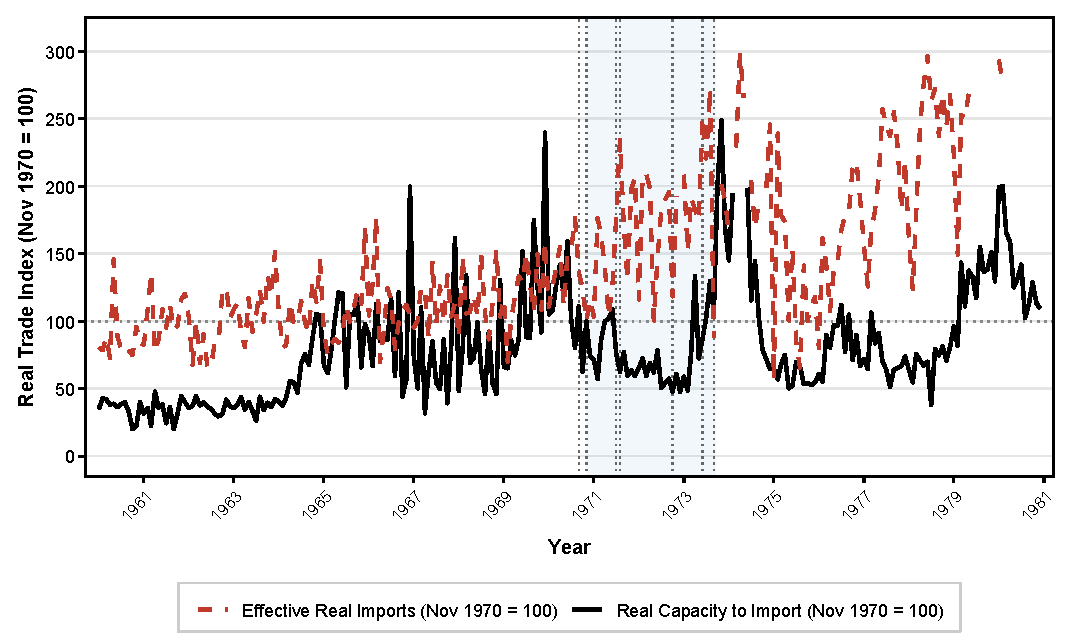
\includegraphics[width=0.88\textwidth]{figures/fig01f_import_capacity.pdf}
\begin{minipage}{0.95\textwidth}
\vspace{0.2cm}
\footnotesize
\textbf{Notes:} Monthly trajectory tracking the Prebisch-ECLAC Real Capacity to Import ($M^{\text{cap}}_t \equiv [\text{Exports}_t / \text{Exports}_{70:11}] \times [(P^{\text{Cu}}_t / P^{\text{Cu}}_{70:11}) / (P^{\text{US}}_{W,t} / P^{\text{US}}_{W,70:11})] \times 100$, solid black line) against Effective Real Imports ($M_t \equiv \text{Imports}_t / \text{Imports}_{70:11} \times 100$, dashed red line). Both series normalized to November 1970 = 100. Benchmark markers $\mathrm{I}$--$\mathrm{VII}$ defined in Table~\ref{tab:critical_junctures}. Shaded blue region designates the Unidad Popular government (1970--1973). Physical merchandise export and import volume series sourced from \citet{DiazBahamonde2023} historical database, compiled from \textit{Estad\'{\i}stica Chilena} and customs records (with April 1973 administrative registration drop interpolated); copper prices from LME via Central Bank of Chile REST API; U.S. wholesale prices from BLS.
\end{minipage}
\end{figure}

Figure~\ref{fig:import_capacity} compares external purchasing power with effective real import flows. When the world price of copper rose from $\$0.508$/lb in January 1973 to $\$0.948$/lb in August 1973, Central Bank gross international reserves remained low, fluctuating in a narrow range of $\$103$--$\$114$ million. The divergence reflected two offsetting movements. On the export side, transport disruptions and equipment shortages held back physical export volumes, muting the revenue gains from higher dollar copper prices. On the import side, effective real imports ($M_t$) expanded, reaching $234.5\%$ of the November 1970 baseline in August 1971 and $272.3\%$ in August 1973, driven by purchases of food, fuel, and intermediate goods.

Operationalizing the Prebisch-ECLAC Capacity to Import ($M^{\text{cap}}_t$), Figure~\ref{fig:import_capacity} documents that Chile's real export purchasing power fell from $100.0$ in November 1970 to $62.5$ in August 1971 and $47.7$ in October 1972 before rebounding in 1973. This generated a wide Real Structural Imbalance ($\Theta_t \equiv M_t / M^{\text{cap}}_t \times 100$), which reached $374.9\%$ in August 1971 and $346.4\%$ in December 1971 (Table~\ref{tab:marglin_monthly_grounding}). The descriptive sequence demonstrates that external balance-of-payments pressures and foreign-exchange scarcity were present well before the price acceleration of late 1972.

\subsubsection{Nominal Dynamics: Money Growth, Inflation, and Multiplier Compression}
\label{sec:stylized_nominal_dynamics}

Figures~\ref{fig:money_growth_inflation} and \ref{fig:money_multiplier} evaluate the high-frequency co-movement between monetary growth, consumer price inflation, and the broad-to-base money multiplier across 1960--1980.

\begin{figure}[!htbp]
\centering
\caption{Monetary Expansion Rates and Monthly Consumer Inflation (1960--1980)}
\label{fig:money_growth_inflation}
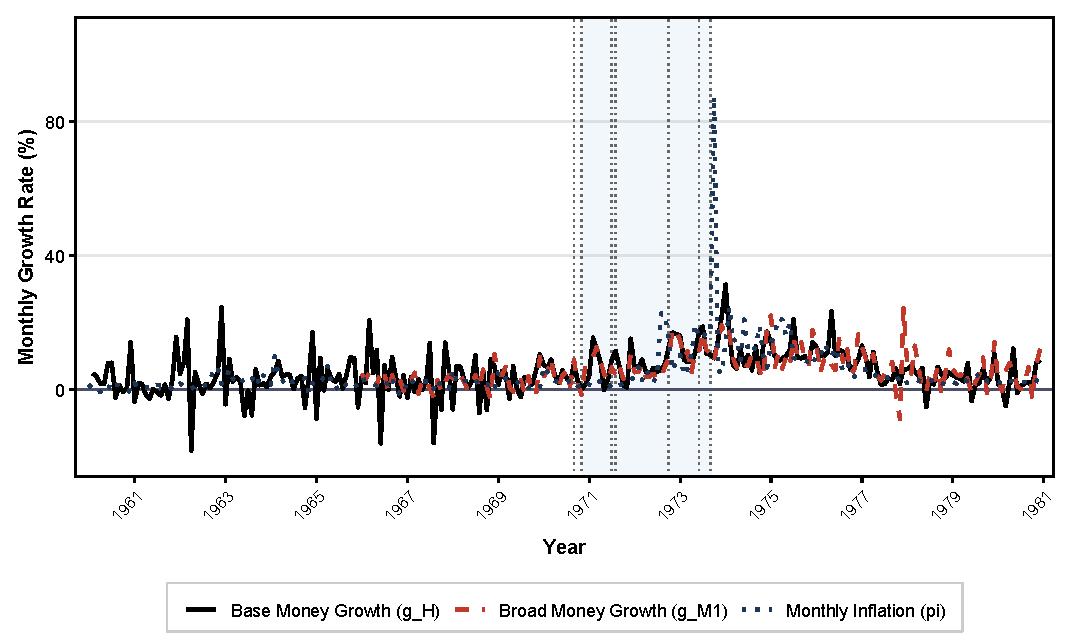
\includegraphics[width=0.88\textwidth]{figures/fig01d_money_growth_inflation.pdf}
\begin{minipage}{0.95\textwidth}
\vspace{0.2cm}
\footnotesize
\textbf{Notes:} Monthly series of base money growth ($g_{H,t}$, solid black line), broad money supply growth ($g_{M1,t}$, dashed red line), and monthly consumer price inflation ($\pi_t$, dotted blue line). Benchmark markers $\mathrm{I}$--$\mathrm{VII}$ defined in Table~\ref{tab:critical_junctures}. Shaded blue region designates the Unidad Popular government (1970--1973). Sourced from Banco Central de Chile REST API and Instituto Nacional de Estad\'{\i}sticas (INE).
\end{minipage}
\end{figure}

\begin{figure}[!htbp]
\centering
\caption{Observed Empirical Money Multiplier ($M1/H$, 1965--1980)}
\label{fig:money_multiplier}
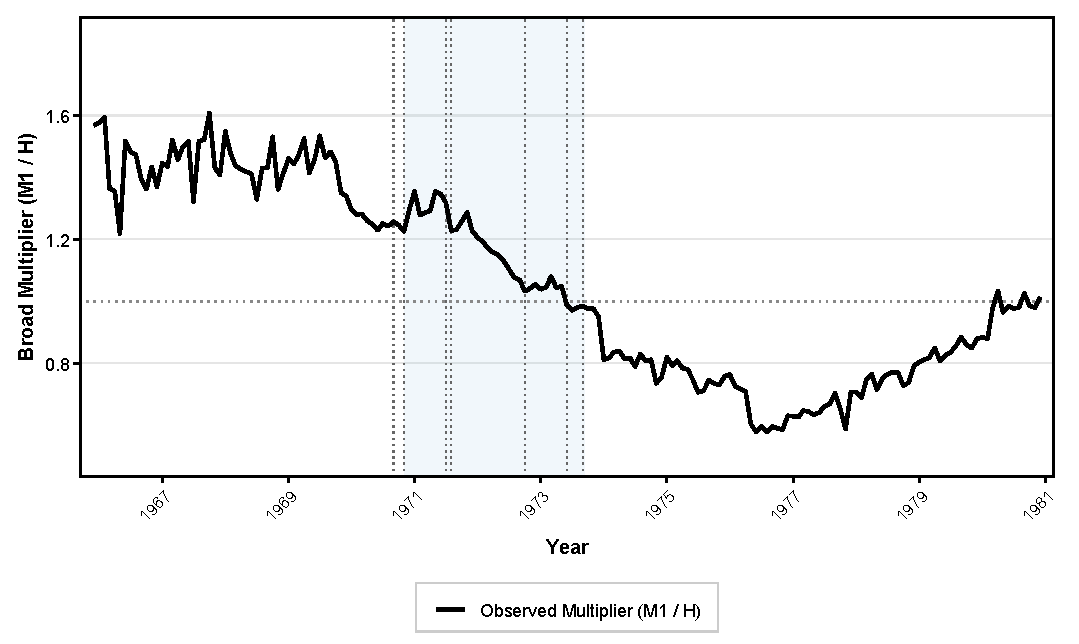
\includegraphics[width=0.88\textwidth]{figures/fig01e_money_multiplier.pdf}
\begin{minipage}{0.95\textwidth}
\vspace{0.2cm}
\footnotesize
\textbf{Notes:} Monthly trajectory of the broad-to-base money multiplier ($m_t \equiv M1_t / H_t$, solid black line). The figure is restricted to the observed M1 sample, December 1965--December 1980. Benchmark markers $\mathrm{I}$--$\mathrm{VII}$ defined in Table~\ref{tab:critical_junctures}. Shaded blue region designates the Unidad Popular government (1970--1973). Sourced from Banco Central de Chile REST API.
\end{minipage}
\end{figure}

In Figure~\ref{fig:money_growth_inflation}, base money ($g_H$) and broad money ($g_{M1}$) grew at monthly rates of $10\%\text{--}15\%$ through 1971 and early 1972, while physical manufacturing output expanded and wages rose. Monthly consumer inflation remained below $5\%$ during this initial phase, rising to $15.2\%$ in October 1972 as transport disruptions and commercial withholding emerged during the nationwide trucking strike. Central bank credit expansion accompanied rising enterprise operating costs and payroll requirements in subsequent months. The monthly peak of consumer inflation occurred in October 1973 ($+87.6\%$) following the military junta's Decree Law 522 price deregulation. This descriptive sequence is consistent with credit accommodation of cost pressures; Section~\ref{sec:granger_tournament} tests whether that directional relationship holds systematically.

Figure~\ref{fig:money_multiplier} tracks the empirical broad-to-base money multiplier ($m_t \equiv M1_t / H_t$). Under Frei (1966--1970), the multiplier fluctuated between $1.35$ and $1.60$. Under the UP administration, the ratio trended downward from $1.35$ in January 1971 to $0.98$ in August 1973, reaching a low of $0.58$ in 1976. Accelerating inflation co-moves visually with this compression in the broad-to-base ratio. Possible institutional mechanisms underlying this decline---including cash hoarding during shortages and central bank credit to socialized firms---are discussed in Sections~\ref{sec:macro_framework} and \ref{sec:discussion_conclusion}; Section~\ref{sec:granger_tournament} evaluates its predictive precedence relative to inflation.

\subsubsection{Real Production Divergence and Focused Monthly Windows}
\label{sec:stylized_real_production}

Figure~\ref{fig:manufacturing_mining} plots physical output dynamics across 1960--1980, documenting divergent paths between domestic manufacturing and export mining.

\begin{figure}[!htbp]
\centering
\caption{Real Physical Output Trajectories: Manufacturing vs. Mining (1960--1980)}
\label{fig:manufacturing_mining}
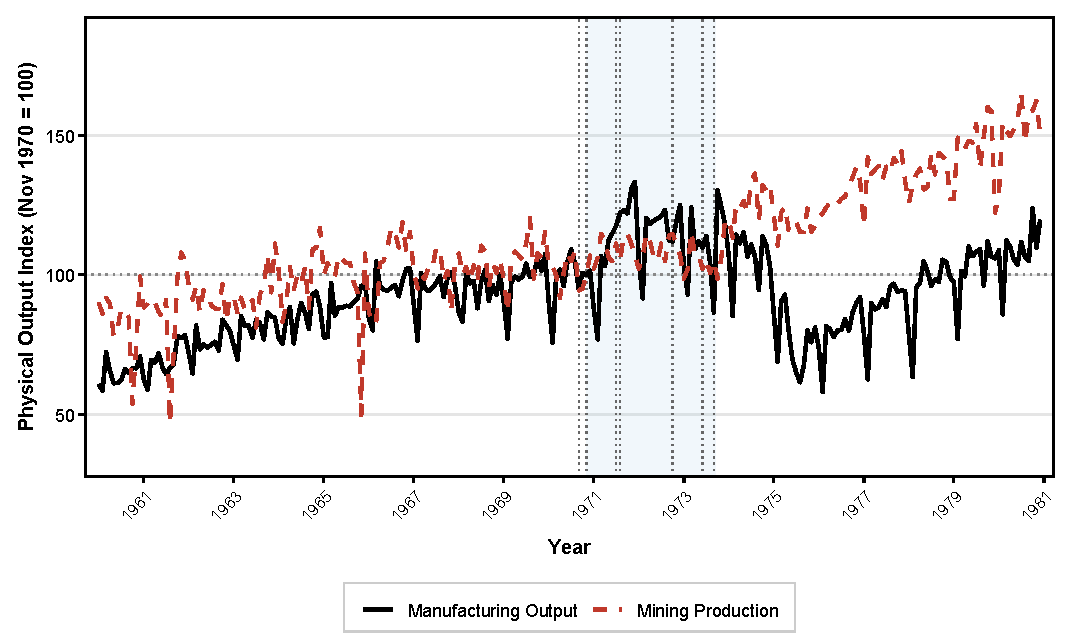
\includegraphics[width=0.88\textwidth]{figures/fig01c_manufacturing_mining.pdf}
\begin{minipage}{0.95\textwidth}
\vspace{0.2cm}
\footnotesize
\textbf{Notes:} Monthly series of physical output indices for manufacturing (solid black line) and mining (dashed red line), re-based to November 1970 = 100. Benchmark markers $\mathrm{I}$--$\mathrm{VII}$ defined in Table~\ref{tab:critical_junctures}. Shaded blue region designates the Unidad Popular government (1970--1973). Sourced from \citet{DiazBahamonde2023} historical database, compiled from INE and SOFOFA for manufacturing, and SERNAGEOMIN, ODEPLAN, and CODELCO for mining.
\end{minipage}
\end{figure}

Manufacturing output expanded by $33.3\%$ between November 1970 and December 1971, reflecting utilization of capacity in wage-goods industries. In contrast, copper mining output rose by $7.0\%$, held back by technical constraints and equipment import delays \citep{DeVylder1976}. Following the October 1972 strike, manufacturing output contracted as transport disruptions and intermediate input shortages took effect. Following the September 1973 coup, manufacturing production declined persistently, falling below index 65 by 1975 (a $>35\%$ contraction from its 1971 peak) amid tariff reductions and demand compression.

Figure~\ref{fig:event_windows} examines monthly dynamics around two institutional turning points.

\begin{figure}[!htbp]
\centering
\begin{subfigure}[b]{0.85\textwidth}
    \centering
    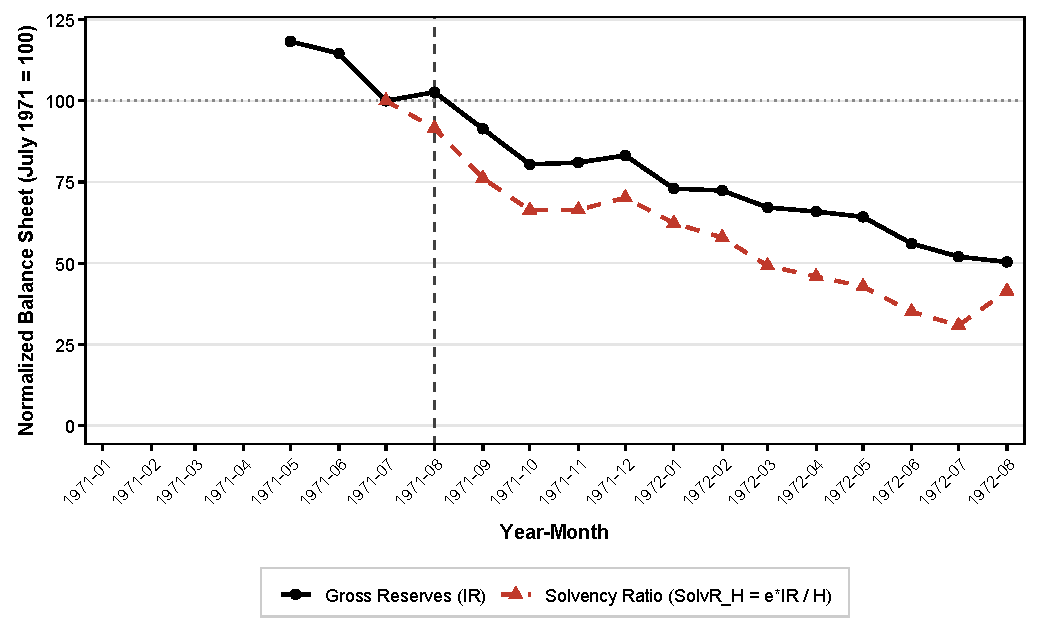
\includegraphics[width=\textwidth]{figures/fig02a_event_blockade_1971.pdf}
    \caption{August 1971 Credit Restrictions and Gold Suspension}
    \label{fig:event_blockade_1971}
\end{subfigure}
\vspace{0.3cm}

\begin{subfigure}[b]{0.85\textwidth}
    \centering
    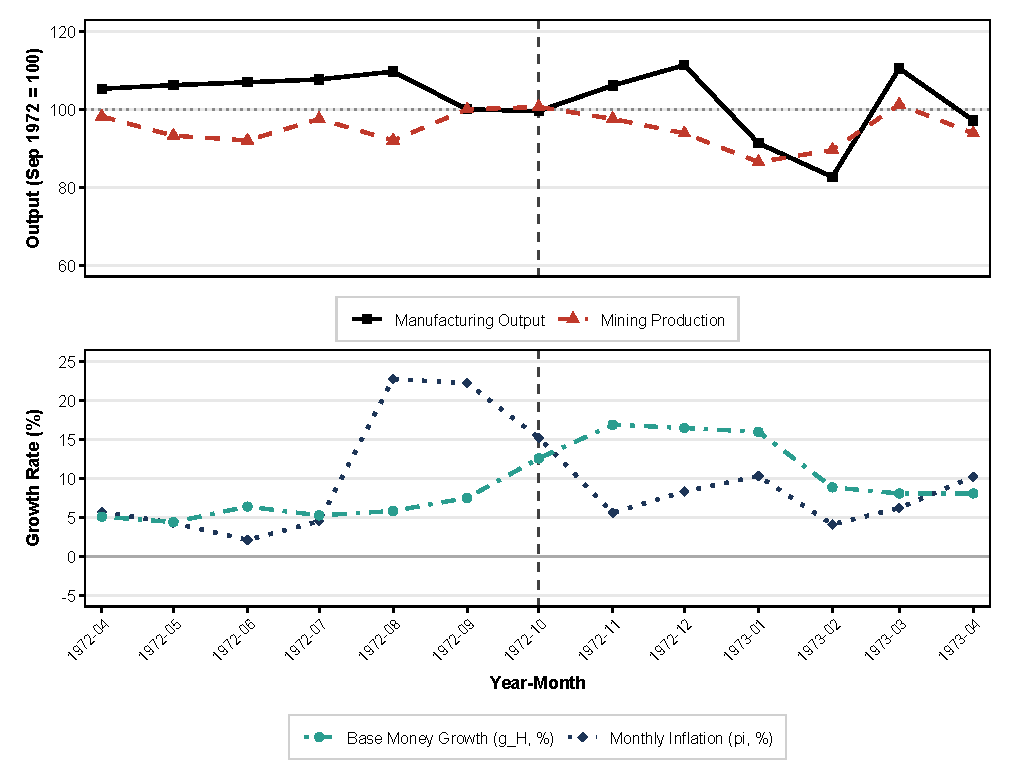
\includegraphics[width=\textwidth]{figures/fig02b_event_lockout_1972.pdf}
    \caption{October 1972 Lockout and Trucking Strike}
    \label{fig:event_lockout_1972}
\end{subfigure}
\caption{Monthly Trajectories around External and Supply Shocks (Chile, 1971--1972)}
\label{fig:event_windows}
\vspace{0.2cm}
\begin{minipage}{0.95\textwidth}
\footnotesize
\textbf{Notes:} Monthly series centered at $t=0$ around two institutional turning points. Panel~(a) tracks Central Bank Gross International Reserves ($IR_t$, solid black line with circle markers) and the Solvency Ratio relative to Base Money ($\text{SolvR}^{H}_t \equiv \frac{e_t \cdot IR_t}{H_t \cdot 1000}$, dashed red line with triangle markers), indexed to July 1971 = 100, around the August 1971 Eximbank credit denial and Bretton Woods gold-window suspension (Benchmark $\mathrm{IV}$). Panel~(b) aligns two vertical subpanels around the October 1972 Lockout (Benchmark $\mathrm{V}$): the upper panel displays physical output indices for Manufacturing (solid black line with square markers) and Mining Production (dashed red line with triangle markers), indexed to September 1972 = 100; the lower panel displays monthly consumer inflation ($\pi_t$, dotted dark-blue line with diamond markers) and Central Bank base money growth ($g_H$, dot-dashed teal line with circle markers) in genuine monthly growth percentages ($\%$) along a common horizontal time axis. Sourced from Banco Central de Chile REST API, IMF International Financial Statistics, and \citet{DiazBahamonde2023}.
\end{minipage}
\end{figure}

The first window centers on the August 1971 credit restrictions and suspension of dollar-gold convertibility (Figure~\ref{fig:event_blockade_1971}, $t=0$). Following the constitutional copper nationalization of July 11, the U.S. Export-Import Bank denied credit on August 12, and President Nixon suspended dollar-gold convertibility on August 15 \citep{Zoeller2019}. This monthly window illustrates the trajectory of reserve drain: gross international reserves fell from index $100.0$ to below $30.0$, and the Central Bank Solvency Ratio ($\text{SolvR}^{H}_t$) declined by more than $70\%$ over the subsequent twelve months. Reserve coverage had deteriorated substantially before the later acceleration in domestic money growth.

The second window centers on the October 1972 trucking strike and commercial lockout (Figure~\ref{fig:event_lockout_1972}, $t=0$). Transport paralysis and merchant shutdowns coincided with a 12 percentage-point drop in manufacturing output, while mining output in northern enclaves remained less affected. Monthly consumer inflation rose from $2.8\%$ to $15.2\%$. Base-money growth did not accelerate contemporaneously with the October jump in inflation; its acceleration followed at $t = +1$ and $t = +2$. The descriptive window places the price increase before the subsequent expansion in base-money growth. While this ordering is consistent with accommodation of cost pressures, establishing directional precedence requires the econometric testing developed below.

\subsubsection{Descriptive Synthesis and Empirical Transition}
\label{sec:stylized_synthesis}

Table~\ref{tab:marglin_monthly_grounding} presents macroeconomic indicators across six selected dates, and Table~\ref{tab:critical_junctures} summarizes the seven institutional events ($\mathrm{I}$--$\mathrm{VII}$).

\begin{table}[H]
\centering
\small
\caption{Monthly Macroeconomic Dynamics, Central Bank Solvency, and External Constraints across Structural Junctures (Chile, 1970--1973)}
\label{tab:marglin_monthly_grounding}
\label{tab:marglin_grounding}
\renewcommand{\arraystretch}{1.10}
\setlength{\tabcolsep}{4.8pt}
\resizebox{\textwidth}{!}{%
\begin{tabular}{lcccccc}
\toprule
& \textbf{Nov 1970} & \textbf{Aug 1971} & \textbf{Dec 1971} & \textbf{Oct 1972} & \textbf{Aug 1973} & \textbf{Dec 1973} \\
\textbf{Macroeconomic Variable} & \textit{Inauguration} & \textit{Gold Suspension} & \textit{Output Peak} & \textit{October Lockout} & \textit{Pre-Coup} & \textit{Post-Coup} \\
\midrule
\multicolumn{7}{l}{\textbf{A. Inflation and Price Dynamics}} \\[0.2em]
Monthly Inflation (\%) & 0.6\% & 1.1\% & 2.8\% & 15.2\% & 17.1\% & 4.7\% \\
YoY Inflation (\%) & 35.3\% & 17.4\% & 22.1\% & 142.9\% & 303.6\% & 508.1\% \\
\midrule
\multicolumn{7}{l}{\textbf{B. Real Physical Activity (Nov 1970 = 100)}} \\[0.2em]
Manufacturing Output Index & 100.0 & 122.0 & 133.3 & 111.9 & 104.6 & 118.1 \\
Mining Production Index & 100.0 & 104.9 & 107.0 & 114.7 & 100.7 & 119.6 \\
\midrule
\multicolumn{7}{l}{\textbf{C. Central Bank Solvency and Monetary Backing}} \\[0.2em]
Gross International Reserves (USD M) & 408.0 & 268.1 & 217.2 & 103.4 & 114.2 & 179.7 \\
Solvency Ratio Base ($\text{SolvR}^H \equiv \frac{e \cdot IR}{H \cdot 1000}$) & 0.63 & 0.22 & 0.17 & 0.07 & 0.06 & 0.25 \\
Solvency Ratio M1 ($\text{SolvR}^{M1} \equiv \frac{e \cdot IR}{M1 \cdot 1000}$) & 0.51 & 0.18 & 0.14 & 0.07 & 0.06 & 0.27 \\
Observed Multiplier ($M1/H$) & 1.23 & 1.23 & 1.23 & 1.03 & 0.98 & 0.95 \\
Base Money Monthly Growth ($g_H$) & 0.0\% & 11.5\% & 15.1\% & 12.6\% & 10.7\% & 21.8\% \\
M1 Money Monthly Growth ($g_{M1}$) & -1.6\% & 4.3\% & 10.2\% & 9.1\% & 11.6\% & 19.2\% \\
\midrule
\multicolumn{7}{l}{\textbf{D. Official Exchange Rate and World Commodity Prices}} \\[0.2em]
Official Exchange Rate ($e_t$) & 0.012 & 0.0122 & 0.0146 & 0.0250 & 0.0740 & 0.34 \\
World Copper Price (USD/lb) & \$0.492 & \$0.499 & \$0.471 & \$0.466 & \$0.948 & \$1.011 \\
World Gold Price (USD/oz) & \$37.44 & \$42.71 & \$43.48 & \$64.86 & \$106.76 & \$106.72 \\
\midrule
\multicolumn{7}{l}{\textbf{E. External Trade, Capacity to Import, and Structural Imbalance}} \\[0.2em]
Export Activity Index & 2.68 & 1.71 & 1.73 & 1.46 & 2.31 & 2.81 \\
Import Activity Index & 1.51 & 3.54 & 3.11 & 1.79 & 4.11 & 2.86 \\
Real Trade Ratio ($\text{Exp}/\text{Imp}$) & 1.78 & 0.48 & 0.56 & 0.82 & 0.56 & 0.98 \\
Real Capacity to Import ($M^{\text{cap}}_t$, Nov 1970 = 100) & 100.0 & 62.5 & 59.5 & 47.7 & 129.5 & 168.7 \\
Effective Real Imports ($M_t$, Nov 1970 = 100) & 100.0 & 234.5 & 206.2 & 118.4 & 272.3 & 189.4 \\
Real Structural Imbalance ($\Theta_t$, \%) & 100.0\% & 374.9\% & 346.4\% & 248.1\% & 210.3\% & 112.3\% \\
US Wholesale Price Index (Nov 1970 = 100) & 100.0 & 103.8 & 104.0 & 108.1 & 128.0 & 127.8 \\
\bottomrule
\end{tabular}%
}
\vspace{0.3em}
\begin{minipage}{\textwidth}
\footnotesize \textbf{Sources and Notes:} Primary monthly series from Central Bank of Chile and IMF International Financial Statistics. Gross international reserves ($IR_t$) represent official foreign exchange holdings from IMF IFS. Solvency Ratio defined relative to Base Money as $\text{SolvR}^{H}_t \equiv (e_t \cdot IR_t) / (H_t \cdot 1000)$ and relative to M1 as $\text{SolvR}^{M1}_t \equiv (e_t \cdot IR_t) / (M1_t \cdot 1000)$, where $IR_t$ is in USD millions, $e_t$ is the official exchange rate in pesos per USD (standardized per BCCh historical conventions), and $H_t, M1_t$ are recorded in thousands of millions of pesos (billions, \emph{miles de millones de pesos}), scaled by $1{,}000$ to express monetary liabilities in millions of pesos and ensure dimensional consistency with the numerator ($e_t \cdot IR_t$). Capacity to Import Index operationalizes the Prebisch-ECLAC formula: $M^{\text{cap}}_t \equiv (\text{Exports}_t / \text{Exports}_{70:11}) \times [(P^{\text{Cu}}_t / P^{\text{Cu}}_{70:11}) / (P^{\text{US}}_{W,t} / P^{\text{US}}_{W,70:11})] \times 100$. Real Structural Imbalance Ratio defined as $\Theta_t \equiv (M_t / M^{\text{cap}}_t) \times 100$, tracking the physical quantum of imports relative to real export purchasing power. Selected dates mark historical milestones: Nov 1970 (Allende inauguration baseline); Aug 1971 (Eximbank credit denial and suspension of dollar-gold convertibility); Dec 1971 (cyclical output peak); Oct 1972 (national trucking strike and commercial lockout); Aug 1973 (late administration baseline before the September coup); and Dec 1973 (post-coup benchmark following October 1973 Decree Law 522 price deregulation).
\end{minipage}
\end{table}


\begin{table}[H]
\centering
\small
\caption{Chronology of Critical Macroeconomic Junctures and Institutional Shocks (Chile, 1970--1973)}
\label{tab:critical_junctures}
\renewcommand{\arraystretch}{1.15}
\resizebox{\textwidth}{!}{%
\begin{tabular}{clllp{6.8cm}}
\toprule
\textbf{Ref} & \textbf{Date} & \textbf{Historical Juncture} & \textbf{Institutional Shock Mechanism} & \textbf{Macroeconomic / Balance-Sheet Transmission Channel} \\
\midrule
$\mathrm{I}$   & Sep 1970 & Presidential Election & Electoral panic; commercial deposit runs & Capital flight ($EO < 0$); foreign currency accumulation; Central Bank emergency rediscounts. \\
$\mathrm{II}$  & Nov 1970 & Inauguration Baseline & Allende assumes presidency; tariff and price freeze & Initial price stabilization; real wage gains; inherited gross reserve buffer (\$408.0M; $\text{SolvR}^H = 0.63$; $\text{SolvR}^{M1} = 0.51$). \\
$\mathrm{III}$ & Jul 1971 & Copper Nationalization & Unanimous constitutional reform (Law 17,450) & Sovereign recovery of \textit{Gran Miner\'ia}; triggers bilateral U.S. credit restrictions and legal liens. \\
$\mathrm{IV}$  & Aug 1971 & Eximbank Embargo \& Bretton Woods Collapse & U.S. credit freeze; dollar-gold convertibility suspended & Revolving trade credits reduced (\$220M $\to$ \$35M); cash-in-advance imports; reserve drain accelerates ($\Delta IR = -\$140$M). \\
$\mathrm{V}$   & Oct 1972 & October Lockout (\textit{Paro de Octubre}) & Trucking strike; SOFOFA commercial lockout & Physical transport paralysis; wholesale inventory withholding; monthly inflation rises to $15.2\%$; central bank liquidity accommodation. \\
$\mathrm{VI}$  & Jun 1973 & \textit{El Tanquetazo} & Military uprising (2nd Armored Regiment) & Heightened political instability; logistical disruption; black market expansion; reserve depletion and structural trade imbalance ($\Theta_t = 210.3\%$). \\
$\mathrm{VII}$ & Sep 1973 & Military Coup d'\'Etat & Violent overthrow; followed by October DL 522 deregulation & Elimination of price controls; $+87.6\%$ MoM inflation jump in October; real wage contraction ($-40\%$); domestic expenditure compression. \\
\bottomrule
\end{tabular}%
}
\begin{tabular}{p{0.95\textwidth}}
\footnotesize \textbf{Notes:} Master reference chronology for vertical benchmark lines appearing across high-frequency time series (Figures~\ref{fig:solvency_reserves}--\ref{fig:money_multiplier}) and defining intervention cutoffs for focused monthly windows (Figures~\ref{fig:event_blockade_1971}--\ref{fig:event_lockout_1972}) and companion econometric estimation stages.
\end{tabular}
\end{table}


Table~\ref{tab:marglin_monthly_grounding} illustrates this temporal sequence across the selected dates: between November 1970 and August 1971---while monthly consumer inflation remained low ($1.1\%$) and industrial manufacturing output was expanding ($+22.0\%$)---the Central Bank Solvency Ratio ($\text{SolvR}^{H}_t$) had declined from $0.63$ to $0.22$, and gross foreign reserves had fallen by $\$139.9$ million. External balance-of-payments deterioration preceded the subsequent acceleration of domestic inflation and credit expansion.

Across the selected dates, reserve coverage deteriorated substantially before the sharp acceleration of inflation in late 1972. Money growth, inflation, exchange-rate adjustment, and trade imbalances moved together during much of the crisis, so these descriptive sequences do not establish their direction of dependence. Section~\ref{sec:granger_tournament} evaluates directional predictive precedence through Granger-causality tests in stationary vector autoregressions across six modular empirical systems. Section~\ref{sec:tvar_solvency_regimes} then estimates a non-linear Threshold Vector Autoregression (TVAR) conditioned on the monthly Solvency Growth Gap ($\Delta s_{t-1} \equiv g^F_{t-1} - g^H_{t-1}$) to test whether these relationships change under conditions of central bank insolvency.



\subsection{Empirical Exercise 1: Directional Precedence and Monetary Accommodation in Stationary Vector Autoregressions}
\label{sec:granger_tournament}
\label{sec:granger_linear}

\subsubsection{Econometric Framework and Evidential Standard}
\label{sec:granger_methodology}
\label{sec:granger_unit_root}
\label{sec:granger_tournament_setup}

The stylized facts documented in Section~\ref{sec:stylized_facts} leave open a central empirical question: did domestic monetary expansion precede price acceleration as an autonomous impulse, or did it accommodate price pressures, enterprise working-capital requirements, and external balance-of-payments constraints? Standard monetarist accounts treat money creation as an autonomous driver, implying that high-powered reserve money ($g_{H,t}$) and narrow transactions balances ($g_{M1,t}$) should expand without predictive feedback from consumer prices ($\pi_t$) or external shocks:
\begin{equation}
    \mathcal{H}_0^{\text{Exogenous}}: \quad \pi_{t-k} \not\longrightarrow g_{M,t} \quad \text{and} \quad \text{External Shock}_{t-k} \not\longrightarrow g_{M,t} \quad \forall k \ge 1.
    \label{eq:null_exogeneity}
\end{equation}
In contrast, structuralist and endogenous-money frameworks view money creation as an accommodating response to enterprise cost pressures and balance-of-payments disruptions. When enterprises face escalating nominal costs under price controls and supply bottlenecks, working-capital requirements expand. If the monetary authority accommodates these demands to prevent illiquidity and payroll defaults, temporal predictive precedence should flow from inflation and foreign reserve depletion to domestic money growth ($\pi \to g_H$, $\text{SolvR}^H \to g_H$).

To evaluate these competing temporal sequences, I estimate standard Granger-causality tests within stationary vector autoregressions \citep{Hamilton1994,Lutkepohl2005}. Let $Y_t$ denote a $K \times 1$ vector of stationary transformed macroeconomic series ($I(0)$). An unrestricted vector autoregression of order $k$, $\text{VAR}(k)$, is specified:
\begin{equation}
    Y_t = c + \sum_{i=1}^k A_i Y_{t-i} + \varepsilon_t, \label{eq:var_spec}
\end{equation}
where $c$ is a vector of constants, $A_i$ are $K \times K$ coefficient matrices, and $\varepsilon_t$ is a vector of white-noise disturbances. In a bivariate representation for $(y_t, x_t)$, the system reduces to:
\begin{align}
    y_t &= \alpha_0 + \sum_{i=1}^k \alpha_{i} y_{t-i} + \sum_{i=1}^k \delta_{i} x_{t-i} + \varepsilon_{1t}, \label{eq:granger_spec1} \\
    x_t &= \beta_0 + \sum_{i=1}^k \beta_{i} x_{t-i} + \sum_{i=1}^k \phi_{i} y_{t-i} + \varepsilon_{2t}. \label{eq:granger_spec2}
\end{align}
The null hypothesis that $x_t$ does not Granger-cause $y_t$ corresponds to the joint exclusion restriction on the lagged coefficients of $x$:
\begin{equation}
    H_0: \quad \delta_{1} = \dots = \delta_{k} = 0.
\end{equation}
Because the entered series are stationary ($I(0)$, as established by the Augmented Dickey--Fuller tests in Table~\ref{tab:adf_order_integration}), this restriction is tested using standard finite-sample $F$-tests:
\begin{equation}
    F = \frac{(\text{RSS}_R - \text{RSS}_U) / k}{\text{RSS}_U / (T - Kk - 1)} \sim F(k, T - Kk - 1),
\end{equation}
where $\text{RSS}_R$ and $\text{RSS}_U$ denote the residual sums of squares from the restricted and unrestricted models, respectively. Rejecting $H_0$ indicates that lagged values of $x_t$ contain incremental predictive information for $y_t$ beyond what is captured by the remaining lagged variables in the system. 

In accordance with the chapter's causal-language contract, Granger causality denotes incremental predictive precedence within a specified stationary information set; it does not by itself establish structural causal identification or policy invariance. Empirical admission to the main text is governed by three diagnostic criteria: (1)~modulus stability ($\max |\lambda_i| < 1$); (2)~system-level residual whitening via the multivariate Breusch--Godfrey Lagrange Multiplier test ($p > 0.05$); and (3)~equation-level residual whitening ($p > 0.05$). Specifications that fail these diagnostic standards are not used for directional inference in the main text.

Table~\ref{tab:system_definitions} defines the system variable vectors, mathematical transformations, sample coverage, and evidence status across the empirical systems.
\begin{table}[htbp]
\centering
\small
\renewcommand{\arraystretch}{0.88}
\caption{System Variable Specification and Evidence Hierarchy}
\label{tab:system_definitions}
\begin{tabularx}{\textwidth}{llcc>{\RaggedRight}X}
\toprule
\textbf{System} & \textbf{Variable Vector $Y^{(s)}_t$} & \textbf{$K$} & \textbf{Evidence Status} & \textbf{Variable Definitions and Historical Sample} \\
\midrule
\multicolumn{5}{l}{\textbf{Core Empirical Specifications (Main Text)}} \\
\midrule
\textbf{System 1} & $[\pi_t, \; g_{H,t}]'$ & 2 & Robust Linear & $\pi_t$: Monthly CPI inflation ($\Delta \ln \text{CPI}_t \times 100$). \newline $g_{H,t}$: Base money growth ($\Delta \ln H_t \times 100$). \newline Sample: 1960:01--1980:12 ($N=250$, usable $N_{\text{eff}}=247$). \\
\addlinespace[0.3em]
\textbf{System 2} & $[\pi_t, \; g_{M1,t}, \; g_{H,t}]'$ & 3 & Qualified Linear & $\pi_t$: CPI inflation. \newline $g_{M1,t}$: Un-spliced narrow money growth ($\Delta \ln M1_t \times 100$). \newline $g_{H,t}$: Base money growth. \newline Sample: 1966:01--1980:12 ($N=180$, usable $N_{\text{eff}}=177$). \\
\addlinespace[0.3em]
\textbf{System 6} & $[g_{\text{SolvR\_H},t}, \; g_{P,\text{gold},t}, \; g_{e,t}, \; g_{H,t}, \; \pi_t]'$ & 5 & Qualified Linear (Pre-73) & $g_{\text{SolvR\_H},t}$: Central bank solvency ratio growth ($\text{SolvR}_t^H \equiv [e_t \cdot \text{IR}_t] / [H_t \cdot 1000]$). \newline $g_{P,\text{gold},t}$: World gold price growth. \newline $g_{e,t}$: Devaluation rate. \newline $g_{H,t}$: Base money growth; $\pi_t$: CPI inflation. \newline Sample: 1960:02--1973:09 ($N_{\text{eff}}=161$). \\
\midrule
\multicolumn{5}{l}{\textbf{Auxiliary and Sensitivity Specifications}} \\
\midrule
\textbf{System 3} & $[\pi_t, \; g_{H,t}, \; \Delta \ln m_t]'$ & 3 & Sensitivity Note & $\Delta \ln m_t$: Banking multiplier growth ($m_t \equiv M1_t / H_t$). Sensitivity check on banking mechanism (1966--1980, $N=180$). \\
\addlinespace[0.3em]
\textbf{System 4} & $[\pi_t, \; g_{H,t}, \; \Delta \ln \Theta_t, \; g_{\text{Manuf},t}, \; g_{\text{Mining},t}]'$ & 5 & Descriptive Only & $\Delta \ln \Theta_t$: Structural import imbalance growth; $g_{\text{Manuf},t}$: Manufacturing; $g_{\text{Mining},t}$: Mining. Retained in Appendix~\ref{app:linear_var_diagnostics}. \\
\addlinespace[0.3em]
\textbf{System 5} & $[g_{P,\text{gold},t}, \; g_{e,t}, \; \Delta \ln \Theta_t, \; g_{H,t}, \; \pi_t]'$ & 5 & Inconclusive & External cost-push boundary vector. Unresolved residual autocorrelation; retained in Appendix~\ref{app:linear_var_diagnostics}. \\
\bottomrule
\end{tabularx}
\begin{minipage}{\textwidth}
\vspace{0.3em}
\footnotesize \textit{Notes:} Monthly series from the Central Bank of Chile (BCCh) historical databases and IMF International Financial Statistics. All variables enter in stationary form ($I(0)$). Classification reflects the empirical architecture lock: Systems 1, 2, and qualified pre-October 1973 System 6 constitute the admissible linear core; System 3 is a sensitivity check; Systems 4 and 5 are documented in Appendix~\ref{app:linear_var_diagnostics}.
\end{minipage}
\end{table}


\subsubsection{Nominal Accommodation: Money and Inflation}
\label{sec:granger_nominal_core}

System 1 evaluates dynamic feedback between consumer price inflation ($\pi_t$) and high-powered base money growth ($g_{H,t}$) over the full monthly sample (1960:01--1980:12, $N=250$, usable $N_{\text{eff}}=247$ at lag 4). At lag order $k=4$, the system satisfies all diagnostic admissibility criteria: companion matrix eigenvalues confirm stability ($\max |\lambda| = 0.730$), the system Breusch--Godfrey test indicates an absence of residual autocorrelation ($\chi^2 = 3.06, p = 0.548$), and equation-level Breusch--Godfrey tests confirm whitening in both the base money equation ($p = 0.467$) and the inflation equation ($p = 0.284$).

As reported in Panel~A of Table~\ref{tab:core_granger_evidence}, Granger causality between inflation and base money growth is bidirectional at $k=4$. The null that inflation does not Granger-cause base money growth is rejected at the 0.1\% level ($F = 15.004, p < 0.0001$), with a positive sum of lag coefficients ($\sum \hat{\beta}_i = +0.680$). In the forward direction, base money growth also Granger-causes inflation ($F = 2.718, p = 0.0305, \sum \hat{\beta}_i = +0.380$). Evaluating results across alternative lag lengths confirms that reverse accommodation ($\pi \to g_H$) commands substantially larger test statistics ($F \in [15.00, 28.32], p < 0.0001$ across $k=1,\dots,4$) and maintains unbroken statistical significance at all horizons. Forward money growth ($g_H \to \pi$) predicts inflation strongly at short horizons ($F = 14.557, p = 0.0002$ at $k=1$; $F = 9.284, p = 0.0001$ at $k=2$), but attenuates as lag length increases (at the SBIC-selected lag $k^*=3$, $\pi \to g_H$ yields $F = 20.318, p < 0.0001$ while $g_H \to \pi$ yields $F = 5.544, p = 0.0011$).

This pattern provides evidence consistent with defensive monetary accommodation under acute price pressures. While high-powered money growth contributed to subsequent price acceleration at short horizons, consumer price inflation exerted strong and persistent predictive feedback on base money creation. The bidirectional finding is difficult to reconcile with the strict monetarist premise of unidirectional money exogeneity, while demonstrating that nominal transmission operated as a reciprocal spiral. System 1 is classified as a \textsc{Robust Linear Result}.

\subsubsection{Commercial Banking and Multiplier Sensitivity}
\label{sec:granger_banking}

System 2 evaluates the commercial banking sector using official un-spliced narrow money balances ($M1$), high-powered base money ($H$), and consumer price inflation over the post-1966 banking window (1966:01--1980:12, $N=180$, usable $N_{\text{eff}}=177$ at $k=3$). At lag $k=3$, the three-variable system satisfies the diagnostic admissibility criteria: the system is stable ($\max |\lambda| = 0.817$), the system Breusch--Godfrey test fails to reject white-noise residuals ($p = 0.428$), and equation-level tests indicate no serial correlation ($p = 0.289$ in the base money equation).

As shown in Panel~B of Table~\ref{tab:core_granger_evidence}, in the diagnostically admissible trivariate VAR(3), narrow-money and base-money growth contain predictive information for one another after conditioning on inflation. Commercial narrow-money growth predicts base-money expansion ($g_{M1} \to g_H$: $F = 3.654, p = 0.0138, \sum \hat{\beta}_i = +0.510$), while base-money growth also predicts narrow money ($g_H \to g_{M1}$: $F = 3.239, p = 0.0236, \sum \hat{\beta}_i = +0.333$). Inflation also predicts subsequent narrow-money growth ($\pi \to g_{M1}$: $F = 6.842, p = 0.0002, \sum \hat{\beta}_i = +0.284$). The reverse relation is not detected once base-money growth is included in the information set: the null that narrow-money growth does not Granger-cause inflation cannot be rejected ($g_{M1} \to \pi$: $F = 1.004, p = 0.3927, \sum \hat{\beta}_i = +0.444$). The banking specification therefore supports predictive interaction between narrow and base money, while the pairwise relation from narrow-money growth to inflation does not survive conditioning on the monetary base. This bilateral dynamic is consistent with an endogenous reserve response to commercial-bank transactions balances, though predictive relations between broad monetary aggregates do not structurally identify credit supply from credit demand. System 2 is classified as a \textsc{Qualified Linear Result}.

\paragraph{Sensitivity Note: Money Multiplier Deconstruction (System 3).}
Deconstructing narrow money into base money and the banking multiplier ($m_t \equiv M1_t / H_t$) evaluates whether multiplier expansion autonomously preceded inflation. In bivariate pairwise tests ($k=1$), multiplier growth displays no predictive information for price inflation ($F = 0.338, p = 0.5617$). When estimated within a conditional VAR(1) containing base money growth, the predictive link $\Delta \ln m \to \pi$ shifts to marginal statistical significance ($F = 3.896, p = 0.0484$). The multiplier result is sensitive to the conditioning set. Because multiplier growth is algebraically related to narrow-money and base-money growth ($\Delta \ln m_t \equiv g_{M1,t} - g_{H,t}$), conditioning on base money growth mathematically incorporates narrow money dynamics, closely reflecting the commercial credit interaction documented in System~2. This specification is therefore treated as a sensitivity check on the banking representation rather than as an independent empirical result, and is classified as \textsc{Specification-Sensitive}.

\subsubsection{Central Bank Solvency Dynamics Before October 1973}
\label{sec:granger_solvency_pre73}

System 6 examines the dynamic interaction between the central bank's foreign solvency backing and domestic macroeconomic aggregates. The system specifies the five-variable vector $Y^{(6)}_t = [g_{\text{SolvR\_H},t}, g_{P,\text{gold},t}, g_{e,t}, g_{H,t}, \pi_t]'$, where $g_{\text{SolvR\_H},t} \equiv \Delta \ln \text{SolvR}^H_t \times 100$ tracks the monthly growth rate of the Solvency Ratio ($\text{SolvR}^H_t \equiv [e_t \cdot \text{IR}_t] / [H_t \cdot 1000]$).

In the full sample (1960:01--1980:12, $N=250$), System 6 fails residual whitening across all tested lag lengths $k \in \{1, \dots, 4\}$ ($p < 0.0001$). Under the chapter's admissibility criteria, the full-sample linear system is not used for directional inference. However, partitioning the sample at the October 1973 institutional break reveals that residual autocorrelation is concentrated in the post-1973 crawling-peg era. In the pre-October 1973 subperiod (1960:02--1973:09, $N_{\text{eff}} = 161$), extending the specification to $k=3$ resolves residual persistence. The pre-1973 conditional VAR(3) is the unique specification across all tested sample partitions that satisfies all serial-admissibility criteria: the companion matrix is stable ($\max |\lambda| = 0.8817$), the system Breusch--Godfrey test indicates white-noise residuals ($\chi^2 = 116.35, df=100, p = 0.1262$), the minimum equation-level Breusch--Godfrey test is satisfied ($p = 0.0557$ in the base money equation), and the 12-month Portmanteau test confirms absence of residual correlation ($p = 0.0754$).

Panel~C of Table~\ref{tab:core_granger_evidence} reports the conditional Granger causality results for this admissible pre-1973 model. Solvency ratio growth predictively Granger-causes base money growth ($F = 6.983, p = 0.0002$), driven by a statistically significant positive coefficient at lag 3 ($\hat{\beta}_3 = +0.0568, p = 0.0033$; sum $\sum \hat{\beta}_i = +0.0153$). In the reverse direction, base money growth predictively Granger-causes solvency ratio growth ($F = 2.951, p = 0.0347$), with a large negative coefficient concentrated at lag 2 ($\hat{\beta}_2 = -0.9775, p = 0.0074$; sum $\sum \hat{\beta}_i = -0.8365$). Because high-powered money enters directly into the denominator of $\text{SolvR}^H_t$, this negative predictive lag is consistent with subsequent deterioration in reserve backing, partly reflecting the mechanical denominator relation rather than offsetting reserve accumulation. Solvency ratio growth also contains predictive information for nominal exchange-rate adjustments ($g_{\text{SolvR\_H}} \to g_e$: $F = 3.073, p = 0.0297, \sum \hat{\beta}_i = +0.129$). Consumer price inflation does not predict solvency growth in this conditional specification ($F = 0.686, p = 0.5618$).

These findings establish a qualified empirical result: prior to October 1973, domestic base money creation predicts a decline in the central bank's foreign solvency ratio (partly reflecting the denominator relation), while foreign solvency dynamics exerted lagged predictive feedback on monetary emission. Because this relationship cleared diagnostic standards only within the pre-October 1973 subperiod and cannot be established as a time-invariant linear law across the full sample, System 6 is classified as a \textsc{Qualified Linear Result (Pre-October 1973 Only)}. The linear specification does not determine whether these predictive relationships vary with the inherited solvency state. Section~\ref{sec:tvar_solvency_regimes} examines that possibility directly.

\begin{table}[htbp]
\centering
\small
\renewcommand{\arraystretch}{0.92}
\caption{Admissible Linear Granger Directional Precedence and Evidence Hierarchy}
\label{tab:core_granger_evidence}
\resizebox{\textwidth}{!}{%
\begin{tabular}{llcccccc}
\toprule
\textbf{Direction Tested} & \textbf{Information Set / Regressors} & \textbf{Lag ($k$)} & \textbf{$F$-Statistic} & \textbf{$p$-value} & \textbf{$\sum \hat{\beta}_i$} & \textbf{Diagnostic Status} & \textbf{Evidence Hierarchy} \\
\midrule
\multicolumn{8}{l}{\textbf{Panel A: System 1 --- Nominal Core (Full Sample, 1960:01--1980:12, $N=250$, $N_{\text{eff}}=247$)}} \\
\midrule
$\pi_t \longrightarrow g_{H,t}$ & $\{\pi_t, g_{H,t}\}$ & 4 & 15.004$^{***}$ & $< 0.0001$ & $+0.680$ & Pass (Sys BG $p=0.548$; Eq $p=0.467$) & \textsc{Robust Linear Result} \\
$g_{H,t} \longrightarrow \pi_t$ & $\{\pi_t, g_{H,t}\}$ & 4 & 2.718$^{**}$ & 0.0305 & $+0.380$ & Pass (Sys BG $p=0.548$; Eq $p=0.467$) & \textsc{Robust Linear Result} \\
\midrule
\multicolumn{8}{l}{\textbf{Panel B: System 2 --- Commercial Banking (M1 Window, 1966:01--1980:12, $N=180$, $N_{\text{eff}}=177$)}} \\
\midrule
$g_{M1,t} \longrightarrow g_{H,t}$ & $\{\pi_t, g_{M1,t}, g_{H,t}\}$ & 3 & 3.654$^{**}$ & 0.0138 & $+0.510$ & Pass (Sys BG $p=0.428$; Eq $p=0.289$) & \textsc{Qualified Linear Result} \\
$g_{H,t} \longrightarrow g_{M1,t}$ & $\{\pi_t, g_{M1,t}, g_{H,t}\}$ & 3 & 3.239$^{**}$ & 0.0236 & $+0.333$ & Pass (Sys BG $p=0.428$; Eq $p=0.289$) & \textsc{Qualified Linear Result} \\
$\pi_t \longrightarrow g_{M1,t}$ & $\{\pi_t, g_{M1,t}, g_{H,t}\}$ & 3 & 6.842$^{***}$ & 0.0002 & $+0.284$ & Pass (Sys BG $p=0.428$; Eq $p=0.289$) & \textsc{Qualified Linear Result} \\
$g_{M1,t} \longrightarrow \pi_t$ & $\{\pi_t, g_{M1,t}, g_{H,t}\}$ & 3 & 1.004 & 0.3927 & $+0.444$ & Pass (Sys BG $p=0.428$; Eq $p=0.289$) & Fail to reject ($p > 0.10$) \\
\midrule
\multicolumn{8}{l}{\textbf{Panel C: System 6 --- Central Bank Solvency Dynamics (Pre-October 1973 Partition, 1960:02--1973:09, $N_{\text{eff}}=161$)}} \\
\midrule
$g_{\text{SolvR\_H},t} \longrightarrow g_{H,t}$ & $\{g_{\text{SolvR\_H}}, g_{P,\text{gold}}, g_e, g_H, \pi\}$ & 3 & 6.983$^{***}$ & 0.0002 & $+0.015$ & Pass (Sys BG $p=0.126$; Min Eq $p=0.056$) & \textsc{Qualified Linear Result} \\
$g_{H,t} \longrightarrow g_{\text{SolvR\_H},t}$ & $\{g_{\text{SolvR\_H}}, g_{P,\text{gold}}, g_e, g_H, \pi\}$ & 3 & 2.951$^{**}$ & 0.0347 & $-0.837$ & Pass (Sys BG $p=0.126$; Min Eq $p=0.056$) & \textsc{Qualified Linear Result} \\
$g_{\text{SolvR\_H},t} \longrightarrow g_{e,t}$ & $\{g_{\text{SolvR\_H}}, g_{P,\text{gold}}, g_e, g_H, \pi\}$ & 3 & 3.073$^{**}$ & 0.0297 & $+0.129$ & Pass (Sys BG $p=0.126$; Min Eq $p=0.056$) & \textsc{Qualified Linear Result} \\
$\pi_t \longrightarrow g_{\text{SolvR\_H},t}$ & $\{g_{\text{SolvR\_H}}, g_{P,\text{gold}}, g_e, g_H, \pi\}$ & 3 & 0.686 & 0.5618 & $+0.667$ & Pass (Sys BG $p=0.126$; Min Eq $p=0.056$) & No predictive relation ($p>0.10$) \\
\bottomrule
\end{tabular}%
}
\begin{minipage}{0.98\textwidth}
\vspace{0.4em}
\footnotesize \textbf{Notes:} Evaluated via standard Granger joint $F$-tests within stationary vector autoregressions on stationary transformed series ($I(0)$). 
Significance: $^{***} p < 0.01$, $^{**} p < 0.05$, $^{*} p < 0.10$. Diagnostic pass requires system-level Breusch--Godfrey residual whitening ($p > 0.05$), minimum equation-level Breusch--Godfrey ($p > 0.05$), and modulus stability ($\max |\lambda| < 1$).
Each panel reports a single unambiguous inferential lag order selected to ensure residual whitening:
Panel~A reports the Nominal Core at $k=4$, where residual autocorrelation is fully resolved (at the SBIC lag $k^*=3$, results are qualitatively identical: $\pi \to g_H$ has $F = 20.318, p < 0.0001$ and $g_H \to \pi$ has $F = 5.544, p = 0.0011$).
Panel~B reports Commercial Banking on un-spliced $M1$ data at $k=3$ within the conditional trivariate VAR(3) $\{\pi_t, g_{M1,t}, g_{H,t}\}$, the lag order achieving residual whitening. At lag $k=3$, narrow-money and base-money growth exhibit bidirectional predictive feedback ($p = 0.0138$ and $p = 0.0236$) and inflation predicts narrow money ($p = 0.0002$), while narrow money does not predict inflation once base money is included in the conditioning set ($F = 1.004, p = 0.3927$). (At SBIC lag $k^*=1$, pairwise estimations yielded $g_{M1} \to g_H: F = 21.453, p < 0.0001$; $g_H \to g_{M1}: F = 15.834, p = 0.0001$; $\pi \to g_{M1}: F = 14.322, p = 0.0002$; $g_{M1} \to \pi: F = 14.004, p = 0.0002$).
Panel~C reports Central Bank Solvency exclusively for the pre-October 1973 subperiod at $k=3$, which is the unique serial-admissible specification across all tested sample partitions (full-sample linear models exhibit persistent residual autocorrelation and are not used for directional inference; see Appendix~\ref{app:linear_var_diagnostics}). In Panel~C, the positive predictive link $g_{\text{SolvR\_H}} \to g_H$ is driven by lag 3 ($\hat{\beta}_3 = +0.057, p = 0.0033$), while base money growth predictively drains the solvency ratio at lag 2 ($\hat{\beta}_2 = -0.978, p = 0.0074$).
In accordance with the causal-language contract, Granger causality denotes incremental predictive precedence within a specified stationary information set and does not establish structural causal identification.
\end{minipage}
\end{table}


\subsubsection{Limits of the Linear Exercise and Unresolved Specifications}
\label{sec:granger_limits}
\label{sec:sign_tournament_synthesis}
\label{sec:granger_diagnostics}

Additional real-sector (System 4: manufacturing and mining) and external-sector (System 5: world gold, exchange rates, and structural trade imbalances) vector autoregressions were estimated as part of the broader empirical battery. Because no specification within lag-length selection over $k \in \{1, \dots, 12\}$, the October 1973 historical partition, or month-of-year seasonal controls satisfied the chapter's residual-admissibility criteria, these models are not admitted to the main text's inferential core. Their exploratory estimates, residual autocorrelation profiles, and complete diagnostic records are preserved for transparency in Appendix~\ref{app:linear_var_diagnostics}.

\subsubsection{Transition to Non-Linear Analysis}
\label{sec:granger_transition}
\label{sec:granger_discussion}

The admissible linear vector autoregressive results establish two key findings: domestic monetary emission operated as an accommodative response to nominal price pressures and commercial-bank credit demand, and external solvency backing interacted with domestic base money prior to October 1973. However, constant-parameter linear models impose time-invariant transmission across fundamentally distinct historical regimes. In a financially subordinate open economy lacking international currency status, the macroeconomic impact of price and credit shocks is likely to differ depending on whether foreign exchange reserves are available to buffer imports or whether the central bank faces reserve exhaustion. The linear results establish selected predictive relationships but do not determine whether their magnitude or persistence varies with inherited external solvency; Section~\ref{sec:tvar_solvency_regimes} examines that question with a threshold specification.

In accordance with the chapter's methodological discipline, this transition is motivated by balance-sheet theory and historical regime sensitivity; the failure of linear specifications to whiten residuals in some systems is treated as an empirical limitation of linear modeling, not as econometric validation of the threshold mechanism. The non-linear model stands entirely on its own balance-sheet derivation, concentrated least squares threshold identification, and bootstrap inference.



\subsection{Empirical Exercise 2: Non-Linear Dynamics under Peripheral Central Bank Solvency Regimes: A Threshold VAR Approach}
\label{sec:tvar_solvency_regimes}
% ==============================================================================
% SECTION 5.4: EMPIRICAL EXERCISE 2: NON-LINEAR DYNAMICS UNDER PERIPHERAL CENTRAL BANK SOLVENCY
% A THRESHOLD VECTOR AUTOREGRESSION APPROACH
% ==============================================================================
% Draft Architecture: First Pass Skeleton and Itemized Contents
% Calibrated to UMass Applied Econometrics & Prose Register Standards

\subsubsection{External Solvency Constraints, Balance-Sheet Dynamics, and Structural Identification}
\label{sec:tvar_specification}

\paragraph{The Solvency Boundary and Macroeconomic Non-Linearity in Dependent Economies.}
The directional precedence tests in Section~\ref{sec:granger_tournament} establish that consumer price inflation exerted persistent predictive feedback on base money expansion, while foreign reserve solvency interacted predictively with base money growth prior to October 1973 (Table~\ref{tab:core_granger_evidence}). Linear vector autoregressions, however, impose time-invariant parameters across fundamentally distinct historical phases. In a financially subordinate open economy lacking international reserve-currency status, convertible foreign exchange reserves ($IR_t$) constitute the ultimate material anchor of domestic policy autonomy. When external reserves are abundant, the monetary authority can buffer domestic employment and intermediate input requirements by absorbing external cost shocks. When foreign exchange reserves are depleted, that insulation mechanism dissolves. 

Under acute foreign exchange scarcity, the transmission of macroeconomic shocks changes discontinuously. Private and state enterprises facing escalating nominal costs for imported spare parts, haul-truck tires, industrial equipment, and basic wage goods could no longer secure foreign letters of credit. To prevent production halts, enterprise illiquidity, and payroll defaults, the Central Bank is compelled into defensive liquidity accommodation. Macroeconomic transmission becomes non-linear: innovations to domestic credit ($g^H_t \to \pi_t$) and nominal price shocks ($\pi_t \to g^H_t$) propagate through distinct structural dynamics depending on whether the monetary authority possesses the hard-currency backing to defend the exchange rate and finance critical imports.

\paragraph{The Solvency Growth Gap: Balance-Sheet Derivation and Economic Interpretation.}
To capture the state of external financial backing, I formalize the Central Bank balance-sheet constraint. Let the Solvency Ratio relative to Central Bank base money liabilities be defined as the dimensionless stock ratio:
\begin{equation}
    S_t \equiv \text{SolvR}^H_t = \frac{F_t}{H_t} = \frac{e_t \cdot IR_t}{H_t \cdot 1000},
    \label{eq:tvar_solv_stock_def}
\end{equation}
where $F_t \equiv e_t \cdot IR_t$ represents the domestic-currency valuation of official international reserves and $H_t$ denotes high-powered reserve money. In discrete time, the stock ratio updates according to the exact multiplicative identity:
\begin{equation}
    S_t = S_{t-1} \exp\left( \frac{g^F_t - g^H_t}{100} \right),
    \label{eq:tvar_stock_flow_update}
\end{equation}
where $g^F_t \equiv \Delta \ln F_t \times 100$ is the monthly growth rate of the domestic-currency reserve stock and $g^H_t \equiv \Delta \ln H_t \times 100$ is the growth rate of high-powered base money. 

Taking natural logarithms and first differences yields the continuous-flow update equation:
\begin{equation}
    \Delta s_t \equiv \Delta \ln S_t \times 100 = g^F_t - g^H_t.
    \label{eq:tvar_solvency_gap_def}
\end{equation}
The variable $\Delta s_t$ defines the \emph{Solvency Growth Gap}. Equation~\eqref{eq:tvar_solvency_gap_def} resolves a major econometric problem. As documented in Section~\ref{sec:tvar_threshold_estimation}, the level stock ratio $S_t$ contains a stochastic trend ($I(1)$), violating the ergodicity requirements of threshold bootstrap inference \citep{Hansen1997,Hansen2000}. By contrast, because $g^F_t$ and $g^H_t$ are stationary percentage changes, their linear combination $\Delta s_t$ is strictly $I(0)$. 

The Solvency Growth Gap also carries clear economic meaning. It tracks the net flow balance between external asset accumulation and domestic liability emission. Because a sovereign monetary authority exercises domestic monopoly over legal tender, central bank insolvency does not describe domestic currency illiquidity; rather, it describes the exhaustion of convertible foreign exchange reserves required to settle balance-of-payments obligations and back domestic high-powered liabilities. When $\Delta s_{t-1} > \gamma$, foreign reserves expand faster than the domestic monetary base, stabilizing the external backing of the currency. When $\Delta s_{t-1} \le \gamma$, domestic credit emission significantly outpaces foreign reserve accumulation. This divergence captures an active entry into conditions of central bank insolvency: the state's capacity to import intermediate goods and food collapses, activating distributive conflict and forcing the monetary authority into defensive accommodation.

\paragraph{The Five-Variable Threshold VAR Specification.}
To model these state-dependent interactions, I specify a five-variable Threshold Vector Autoregression partitioned into a world-money forcing block and a domestic macroeconomic block:
\begin{equation}
    X_t = \begin{bmatrix} g^{gold}_t & \Delta \ln \Theta_t & g^F_t & \pi_{m,t} & g^H_t \end{bmatrix}',
    \label{eq:tvar_variable_vector}
\end{equation}
where $g^{gold}_t$ is the monthly growth rate of the London gold bullion price in US dollars, $\Delta \ln \Theta_t$ is the change in the real structural trade imbalance, $g^F_t$ is the growth rate of domestic-currency international reserves, $\pi_{m,t}$ is monthly consumer price inflation, and $g^H_t$ is Central Bank base money growth. 

The two-regime Threshold VAR with one lag takes the form:
\begin{equation}
    X_t = \mu(s_{t-1}) + A_1(s_{t-1}) X_{t-1} + \varepsilon_t,
    \label{eq:tvar_model_equation}
\end{equation}
where the state indicator $s_{t-1} \in \{0, 1\}$ is governed by the predetermined Solvency Growth Gap relative to the threshold parameter $\gamma$:
\begin{equation}
    s_{t-1} = \begin{cases} 
        1 \quad (\text{Adverse Solvency-Growth State}) & \text{if } \Delta s_{t-1} \le \gamma, \\ 
        0 \quad (\text{Non-Adverse State}) & \text{if } \Delta s_{t-1} > \gamma.
    \end{cases}
    \label{eq:tvar_regime_indicator}
\end{equation}
In Equation~\eqref{eq:tvar_model_equation}, $\mu(s_{t-1})$ is a regime-dependent intercept vector, $A_1(s_{t-1})$ is a $5 \times 5$ regime-dependent coefficient matrix, and $\varepsilon_t$ is a vector of white-noise disturbances with regime-specific covariance matrix $\Sigma(s_{t-1})$.

\paragraph{Structural Identification and International Block Exogeneity.}
Contemporaneous structural identification relies on a Cholesky decomposition of the reduced-form covariance matrix. The recursive ordering aligns with institutional timing and international block exogeneity:
\begin{equation}
    g^{gold}_t \longrightarrow \Delta \ln \Theta_t \longrightarrow g^F_t \longrightarrow \pi_{m,t} \longrightarrow g^H_t.
    \label{eq:tvar_cholesky_order}
\end{equation}
This recursive ordering embeds five institutional timing assumptions:
\begin{enumerate}[leftmargin=*,itemsep=1pt]
    \item Global gold price fluctuations reflect international monetary disruptions, including the breakdown of the Bretton Woods system, and do not respond contemporaneously to Chilean macroeconomic shocks.
    \item The real structural trade imbalance ($\Theta_t$) responds to external terms-of-trade shocks before domestic nominal variables adjust.
    \item The domestic-currency reserve flow ($g^F_t$) adjusts to trade settlements and external credit availability within the month.
    \item Domestic consumer prices ($\pi_{m,t}$) respond within the month to import bottlenecks and foreign exchange shortages, but precede high-powered base money creation.
    \item Central Bank base money emission ($g^H_t$) is ordered last, operating as an endogenous accommodation valve that clears enterprise payments and commercial bank liquidity demands within the month.
\end{enumerate}

To avoid in-sample over-fitting, world gold-price growth is treated as block-exogenous in the recursive ordering. This restriction is supported by the absence of detected domestic feedback in the unrestricted TVAR gold equation ($p > 0.10$, Table~\ref{tab:tvar_estimates}) and by the small-open-economy price-taking assumption. I restrict the lag polynomial of the first equation such that all domestic feedback coefficients equal zero:
\begin{equation}
    \begin{bmatrix} g^{gold}_t \\ X^{dom}_t \end{bmatrix} = \begin{bmatrix} \mu_1(s_{t-1}) \\ \mu_2(s_{t-1}) \end{bmatrix} + \begin{bmatrix} a_{11}(s_{t-1}) & \mathbf{0}_{1 \times 4} \\ A_{21}(s_{t-1}) & A_{22}(s_{t-1}) \end{bmatrix} \begin{bmatrix} g^{gold}_{t-1} \\ X^{dom}_{t-1} \end{bmatrix} + \begin{bmatrix} \varepsilon^{gold}_t \\ \varepsilon^{dom}_t \end{bmatrix},
    \label{eq:tvar_block_exogeneity_matrix}
\end{equation}
where $X^{dom}_t = [\Delta \ln \Theta_t, g^F_t, \pi_{m,t}, g^H_t]'$. 


\subsubsection{Testing for Structural Non-Linearity and Solvency Regime Identification}
\label{sec:tvar_threshold_estimation}

\paragraph{Stationarity of the Solvency Flow Gap versus Wandering Reserve Stocks.}
Standard threshold autoregressive models require the transition variable to follow a strictly stationary ergodic process \citep{Hansen1997,Hansen2000}. If a threshold variable contains a stochastic trend ($I(1)$), its empirical density does not cross the boundary with stationary frequency. The series instead wanders away from the threshold for extended historical intervals. Under non-stationarity, standard asymptotic inference collapses, and the threshold search risks identifying spurious chronological breaks rather than recurrent economic states.

Table~\ref{tab:solvency_unit_root} reports the complete stationarity diagnostic battery for both the level stock ratio ($S_t$) and the dynamic flow gap ($\Delta s_t$). For the level solvency ratio, the Augmented Dickey--Fuller test statistic is $-0.564$ ($p = 0.978$), and the Phillips--Perron test statistic is $-1.291$ ($p = 0.983$). Both tests fail to reject the unit-root null hypothesis. The KPSS test likewise rejects the null of level stationarity ($1.726$, $p < 0.01$) and trend stationarity ($0.494$, $p < 0.01$). The level stock $S_t$ is unambiguously an $I(1)$ process.

\begin{table}[htbp]
\centering
\small
\renewcommand{\arraystretch}{0.92}
\caption{Integration Order Diagnostics for Central Bank Solvency Variables (1960:01--1980:12)}
\label{tab:solvency_unit_root}
\label{tab:tab03_solvency_unit_root}
\resizebox{\textwidth}{!}{%
\begin{tabular}{lccccccr}
\toprule
\textbf{Variable / Series} & \multicolumn{2}{c}{\textbf{ADF Test}} & \multicolumn{2}{c}{\textbf{Phillips--Perron}} & \multicolumn{2}{c}{\textbf{KPSS Test}} & \textbf{Order / Classification} \\
\cmidrule(lr){2-3} \cmidrule(lr){4-5} \cmidrule(lr){6-7}
 & \textbf{Stat.} & \textbf{$p$-val} & \textbf{Stat.} & \textbf{$p$-val} & \textbf{Level} & \textbf{Trend} & \\
\midrule
Solvency Ratio ($S_t$, levels) & -0.564 & 0.978 & -1.291 & 0.983 & 1.726$^{***}$ & 0.494$^{***}$ & $I(1)$ (Non-stationary) \\
Solvency Growth Gap ($\Delta s_t$, diff.) & -4.941$^{***}$ & $<0.01$ & -14.011$^{***}$ & $<0.01$ & 0.570$^{*}$ & 0.082 & $I(0)$ (Stationary) \\
\bottomrule
\end{tabular}%
}
\begin{minipage}{\textwidth}
\vspace{0.4em}
\footnotesize \textit{Notes:} Monthly series spanning 1960:01--1980:12 ($N=250$). The level solvency ratio is defined as $S_t \equiv (e_t \cdot IR_t) / (H_t \cdot 1000)$. The Solvency Growth Gap is defined as the exact log difference $\Delta s_t \equiv g^F_t - g^H_t = \Delta \ln S_t \times 100$. Augmented Dickey--Fuller (ADF) tests estimated with constant drift; lag orders selected via Schwarz Bayesian Information Criterion (SBIC). Phillips--Perron (PP) tests employ Newey--West Bartlett kernel bandwidth. For ADF and PP, the null hypothesis is a unit root ($I(1)$); for KPSS, the null hypothesis is stationarity ($I(0)$). Significance: $^{***} p < 0.01$, $^{**} p < 0.05$, $^{*} p < 0.10$. The test battery indicates that the level stock $S_t$ contains a stochastic trend (failing to reject the unit-root null and rejecting KPSS stationarity), whereas the flow growth gap $\Delta s_t$ rejects the unit root and fails to reject trend stationarity, providing evidence consistent with covariance stationarity ($I(0)$) and satisfying the ergodicity preconditions for \citet{Hansen1997,Hansen2000} threshold estimation.
\end{minipage}
\end{table}


By contrast, evaluating the first-differenced Solvency Growth Gap ($\Delta s_t \equiv g^F_t - g^H_t$) yields an Augmented Dickey--Fuller statistic of $-4.941$ ($p < 0.01$) and a Phillips--Perron statistic of $-14.011$ ($p < 0.01$). Both reject the unit-root null hypothesis at the 1\% level. The KPSS test statistic is $0.570$, failing to reject the stationarity null at the 1\% level. The Solvency Growth Gap is stationary ($I(0)$). Specifying $\Delta s_{t-1}$ as the predetermined threshold variable satisfies the relevant integration-order requirement for Hansen threshold estimation.

\paragraph{Concentrated Least Squares Estimation and Rejection of Linearity.}
Having established the stationarity of the transition variable, I estimate the unknown threshold parameter $\gamma$ using concentrated least squares. The estimation algorithm minimizes the determinant of the residual covariance matrix, $\det(\hat{\Sigma}(\gamma))$, across the trimmed empirical support of $\Delta s_{t-1}$. Following \citet{Hansen1999}, I apply a trimming parameter of $\tau = 0.15$, ensuring that every identified regime contains a minimum of 37 monthly observations from the full sample of $N=250$.

Because the threshold parameter $\gamma$ is unidentified under the linear null hypothesis ($H_0: A_1(0) = A_1(1)$), standard likelihood ratio tests follow non-standard asymptotic distributions. To obtain valid inference, I follow \citet{Hansen1999} and implement the Supremum Likelihood Ratio (Sup-LR) test using a residual bootstrap with $B = 1{,}000$ replications. The bootstrap resampling procedure preserves cross-equation contemporaneous error correlation while imposing the linear null restriction.

The resulting test statistic is $\text{Sup-LR} = 112.10$, corresponding to a bootstrap $p$-value of $p = 0.0010$. The bootstrap threshold test rejects the constant-parameter linear specification in favor of the estimated threshold alternative, providing evidence against parameter constancy across the solvency growth gap dimension. The rate at which the monetary authority accumulates foreign reserves relative to domestic liabilities alters the macroeconomic propagation mechanism.

\paragraph{Regime Partition Discipline: Isolating Conditions of Central Bank Insolvency.}
To identify the number of operative regimes, I conduct an unrestricted two-dimensional grid search across candidate thresholds $(\gamma_1, \gamma_2)$. The algorithm isolates two global structural breaks at $\hat{\gamma}_1 = -4.61\%$ and $\hat{\gamma}_2 = +20.87\%$. This partition divides the 250 monthly observations into three distinct economic states:
\begin{enumerate}[leftmargin=*,itemsep=1pt]
    \item \emph{Adverse Solvency-Growth State} ($\Delta s_{t-1} \le -4.61\%$, $N_1 = 100$ months, $40.0\%$ of the sample, reflecting conditions of central-bank insolvency): Base money expansion systematically outpaces foreign reserve accumulation by more than 4.6 percentage points per month.
    \item \emph{Intermediate State} ($-4.61\% < \Delta s_{t-1} \le +20.87\%$, $N_2 = 111$ months, $44.4\%$ of the sample): External reserve growth and domestic credit creation remain within bounded historical corridors.
    \item \emph{High Reserve Accumulation State} ($\Delta s_{t-1} > +20.87\%$, $N_3 = 38$ months, $15.2\%$ of the sample): Rapid foreign exchange accumulation driven by world commodity windfalls.
\end{enumerate}

Although the three-state model captures the upper tail of commodity windfalls, finite-sample constraints dictate careful specification discipline \citep{Hansen1999,Afonso2018}. In a five-variable vector autoregression, each equation requires estimating 7 parameters at $p=1$ and 12 parameters at $p=2$. With only $N_3 = 38$ observations in the high-accumulation regime, degrees of freedom contract to 31 (at $p=1$) and 26 (at $p=2$). Estimating dynamic Generalized Impulse Response Functions on such a small partition induces parameter instability and inflated bootstrap variance.

Because the central objective of this chapter is to examine macroeconomic adjustment under acute foreign exchange depletion rather than commodity windfalls, I adopt a two-regime baseline specification. The model isolates the adverse solvency-growth state ($\Delta s_{t-1} \le -4.615\%$, $N = 100$, degrees of freedom $df = 93$) and pools the remaining observations into a unified non-adverse solvency-growth state ($\Delta s_{t-1} > -4.615\%$, $N = 145$, degrees of freedom $df = 138$). This baseline balances degrees-of-freedom discipline with structural precision, providing a robust empirical foundation for dynamic simulation.

Figure~\ref{fig:regime_timeline} plots the resulting endogenous regime classification across the 1960--1980 timeline, contrasting the persistent level solvency stock ($S_t$) with the stationary flow gap ($\Delta s_t$) and the estimated structural threshold ($\hat{\gamma}_1 = -4.615\%$).

\begin{figure}[htbp]
\centering
\begin{subfigure}[b]{0.49\textwidth}
    \centering
    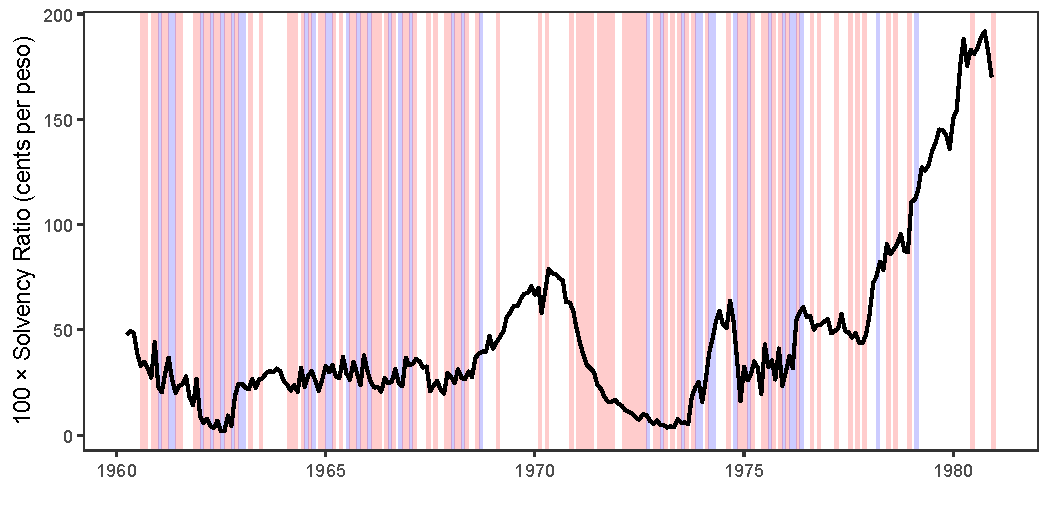
\includegraphics[width=\textwidth]{figures/regime_timeline_level.pdf}
    \caption{Solvency Ratio Stock ($100 \times S_t$)}
    \label{fig:regime_timeline_stock}
\end{subfigure}
\hfill
\begin{subfigure}[b]{0.49\textwidth}
    \centering
    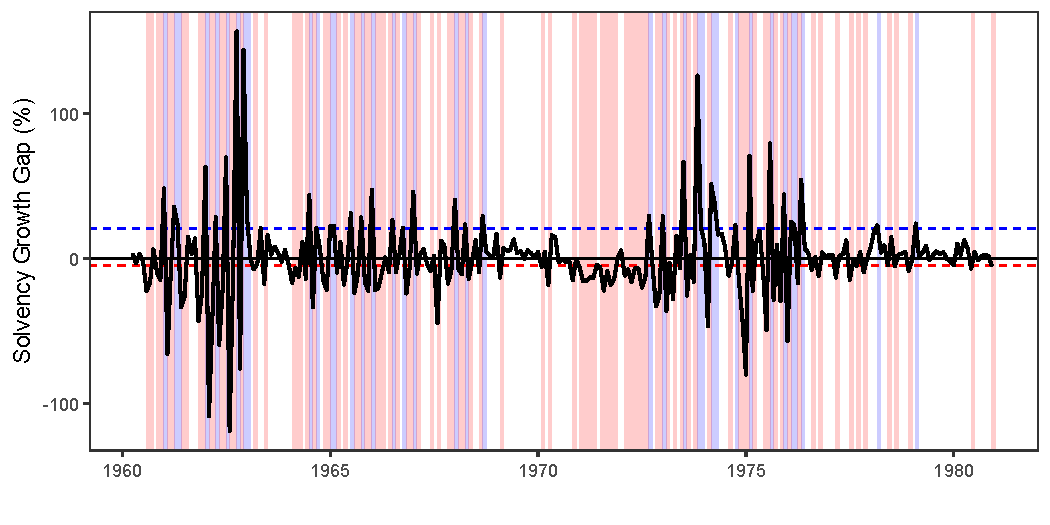
\includegraphics[width=\textwidth]{figures/regime_timeline_gap.pdf}
    \caption{Solvency Growth Gap Flow ($\Delta s_t$)}
    \label{fig:regime_timeline_gap}
\end{subfigure}
\caption{Central Bank Solvency Ratio and Solvency Growth Gap, 1960--1980}
\label{fig:regime_timeline}
\begin{minipage}{\textwidth}
    \vspace{0.3em}
    \footnotesize \textbf{Notes:} \textbf{Panel (A)} displays the monthly Central Bank Solvency Ratio stock ($100 \times S_t \equiv 100 \times [e_t IR_t / (H_t \cdot 1000)]$, expressed as cents per peso). \textbf{Panel (B)} displays the predetermined threshold variable, the Solvency Growth Gap ($\Delta s_t \equiv g^F_t - g^H_t = \Delta \ln S_t \times 100$). Shaded areas distinguish the exploratory three-state diagnostic partition identified by the Concentrated Least Squares grid search: red shading marks the adverse solvency-growth state ($\Delta s_{t-1} \le -4.615\%$, $N=100$), blue shading marks the exploratory upper-tail reserve-accumulation state ($\Delta s_{t-1} > +20.878\%$, $N=38$), and unshaded areas denote the intermediate partition ($N=111$). For econometric estimation and dynamic GIRF simulations, the baseline TVAR pools the two non-adverse partitions into a single unified non-adverse state ($\Delta s_{t-1} > -4.615\%$, $N=145$). The dashed horizontal line in Panel (B) marks the estimated structural threshold ($\hat{\gamma} = -4.615\%$). Data sources: Central Bank of Chile (BCCh) monthly balance sheets (1960:01--1980:12, $N=250$).
\end{minipage}
\end{figure}


\subsubsection{Historical Regime Chronology and the Unidad Popular Trajectory}
\label{sec:tvar_regime_chronology}

\paragraph{Stock-Flow Dynamics: Reserve Exhaustion versus Flow Stabilization.}
The dual-panel trajectory in Figure~\ref{fig:regime_timeline} clarifies the analytical distinction between the level stock of international solvency ($S_t$) and its dynamic flow gap ($\Delta s_t$). Panel~(A) shows that the ratio of official international reserves to Central Bank base money liabilities dropped precipitously in late 1970 and remained near zero throughout 1971--1978. A static stock threshold would classify this entire eight-year window as a single continuous insolvency regime. Such a classification fails to distinguish between active balance-of-payments insolvency and the post-1974 orthodox stabilization under low foreign exchange reserves. Under the military dictatorship, drastic fiscal retrenchment and the contraction of real wages stabilized the flow gap ($\Delta s_t > 0$), despite the depleted stock of reserves.

Panel~(B) demonstrates why the Solvency Growth Gap operates as the true transition trigger. The structural break occurs not when reserve stocks are low in absolute terms, but when base money creation persistently outpaces foreign reserve accumulation. By taking the logarithmic first difference ($\Delta s_t \equiv g^F_t - g^H_t$), the threshold condition $\Delta s_{t-1} \le -4.615\%$ isolates the rate of net reserve depletion. When this gap turns sharply negative, domestic liquidity creation dilutes external reserve backing. The state loses the foreign exchange required to maintain import parities, unanchoring domestic price stability.

\paragraph{Endogenous Dating of the Unidad Popular Macroeconomic Trajectory.}
Without imposing calendar dummies or political intervention dates, the threshold condition $\Delta s_{t-1} \le -4.615\%$ autonomously classifies the critical junctures of the Unidad Popular administration (1970--1973) into the adverse solvency-growth state (reflecting conditions of central-bank insolvency). The mathematical threshold search identifies five distinct historical episodes:
\begin{enumerate}[leftmargin=*,itemsep=1pt]
    \item \emph{November 1970:} Immediate post-electoral capital flight following Salvador Allende's victory triggers an initial gap of $\Delta s_t = -15.18\%$, reflecting commercial bank deposit withdrawals and private asset flight abroad.
    \item \emph{January--May 1971:} The initial redistributive expansion under the Vuskovi\'c Plan drives the growth gap to between $-13\%$ and $-15\%$. High-powered money emission financed public enterprise wage increases while foreign reserves remained stable, initiating the dilution of reserve coverage.
    \item \emph{July--November 1971:} International commercial banks suspended short-term trade credit lines, and US export credit dried up \citep{Stallings1978,DeVylder1976}. The growth gap plunged between $-6\%$ and $-22\%$, reflecting the exhaustion of foreign exchange buffers.
    \item \emph{November--December 1972:} In the aftermath of the October 1972 employer lockout and transport strike \citep[see][]{Casals2021}, the Central Bank extended emergency credit to keep nationalized enterprises operating. The flow gap collapsed to $-26.4\%$ in November and $-33.1\%$ in December.
    \item \emph{February, April, and August 1973:} The final phase of the administration witnessed acute supply bottlenecks for imported spare parts, haul-truck tires, and wheat. With reserves exhausted, the gap reached $-25\%$ to $-36\%$, locking the economy into an accelerating inflation regime.
\end{enumerate}

\paragraph{Endogenous Accommodation versus the Orthodox Narrative of Policy Pathology.}
These empirical findings challenge orthodox accounts of the Chilean transition \citep{DornbuschEdwards1990,Edwards2024}. Mainstream interpretations treat the Unidad Popular inflation as an unforced episode of macroeconomic populism driven by autonomous deficit monetization. In that narrative, monetary policy operates as an independent prime mover unconstrained by external balances. 

The threshold model reveals an alternate institutional mechanism. Monetary emission accelerated defensively to finance enterprise payrolls and purchase essential inputs under strict foreign credit constraints. When foreign commercial banks cut off short-term letters of credit, the state could no longer import intermediate capital goods or food to stabilize domestic markets. Distributive conflict over real income could no longer be pacified through external supply. Under acute reserve depletion, the Central Bank entered an endogenous liquidity accommodation dynamic: price increases required nominal credit expansion to avert enterprise liquidation, which eroded external solvency and amplified inflationary expectations.


\subsubsection{Regime-Dependent Parameter Estimates and Accommodation Dynamics}
\label{sec:tvar_parameter_estimates}

\begin{table}[htbp]
\centering
\small
\renewcommand{\arraystretch}{0.90}
\caption{Regime-Dependent TVAR Parameter Estimates across Solvency Regimes (1960--1980)}
\label{tab:tvar_estimates}
\label{tab:tab04_tvar_estimates}
\resizebox{\textwidth}{!}{%
\begin{tabular}{lccccc}
\toprule
\textbf{Lagged Regressor} & \multicolumn{5}{c}{\textbf{Dependent System Variables ($X_t$)}} \\
\cmidrule(lr){2-6}
 & \textbf{Gold ($g^{gold}_t$)} & \textbf{Imbalance ($\Delta \ln \Theta_t$)} & \textbf{Reserves ($g^F_t$)} & \textbf{Inflation ($\pi_{m,t}$)} & \textbf{Money ($g^H_t$)} \\
\midrule
\multicolumn{6}{l}{\textbf{Panel A: Adverse Solvency-Growth State} ($\Delta s_{t-1} \le -4.615\%$, $N_1 = 100$ months)} \\
\midrule
Constant & 0.636 & -3.720 & 3.388 & -0.300 & 1.893$^{*}$ \\
World Gold Price ($g^{gold}_{t-1}$) & 0.625$^{***}$ & 0.378 & -0.494 & 0.197$^{**}$ & 0.151 \\
Structural Imbalance ($\Delta \ln \Theta_{t-1}$) & --- & -0.188$^{*}$ & --- & 0.010 & --- \\
Reserve Growth ($g^F_{t-1}$) & --- & --- & -0.181 & -0.016 & -0.042 \\
CPI Inflation ($\pi_{m,t-1}$) & --- & --- & 0.512 & 0.684$^{***}$ & 0.581$^{***}$ \\
Base Money Growth ($g^H_{t-1}$) & --- & --- & 0.938 & 0.166$^{***}$ & 0.058 \\
Price Decontrol Dummy ($D_{oct73}$) & -1.225 & 62.520 & 111.026$^{***}$ & 76.213$^{***}$ & -2.775 \\
\midrule
\multicolumn{6}{l}{\textbf{Panel B: Non-Adverse Solvency-Growth State} ($\Delta s_{t-1} > -4.615\%$, $N_2 = 145$ months)} \\
\midrule
Constant & 0.579 & 1.836 & 1.848 & 2.218$^{***}$ & 3.300$^{***}$ \\
World Gold Price ($g^{gold}_{t-1}$) & 0.339$^{***}$ & -1.128$^{**}$ & 0.312 & -0.013 & -0.034 \\
Structural Imbalance ($\Delta \ln \Theta_{t-1}$) & --- & -0.629$^{***}$ & --- & -0.009 & --- \\
Reserve Growth ($g^F_{t-1}$) & --- & --- & -0.355$^{***}$ & -0.014 & 0.006 \\
CPI Inflation ($\pi_{m,t-1}$) & --- & --- & 1.114$^{***}$ & 0.275$^{***}$ & 0.236$^{***}$ \\
Base Money Growth ($g^H_{t-1}$) & --- & --- & -0.173 & 0.240$^{***}$ & 0.115 \\
\bottomrule
\end{tabular}%
}
\begin{minipage}{\textwidth}
\vspace{0.4em}
\footnotesize \textit{Notes:} Monthly series spanning 1960:01--1980:12 ($N=250$, effective sample $T=245$). Conditional Least Squares (CLS) estimates of the five-variable TVAR(1) conditioned on the predetermined Solvency Growth Gap $\Delta s_{t-1} \equiv g^F_{t-1} - g^H_{t-1}$ at the structural threshold $\hat{\gamma} = -4.615\%$. Significance: $^{***} p < 0.01$, $^{**} p < 0.05$, $^{*} p < 0.10$. Dashes (---) denote structural exclusion restrictions: (i) world gold is block exogenous to domestic Chilean variables ($a_{12} = a_{13} = a_{14} = a_{15} = 0$); (ii) real structural imbalance ($\Delta \ln \Theta_t$) is exogenous to domestic feedback ($a_{23} = a_{24} = a_{25} = 0$); and (iii) lagged structural imbalance ($\Delta \ln \Theta_{t-1}$) is excluded from central bank solvency equations ($g^F_t$ and $g^H_t$, $a_{32} = a_{52} = 0$), in accordance with the institutional transmission structure and Latin American structuralist theory. The one-off price decontrol dummy $D_{oct73}$ (Decree Law 522) in Panel A controls for the October 1973 administrative price decontrol and foreign exchange revaluation shock.
\end{minipage}
\end{table}


\paragraph{Equation Estimates and Small-Economy Structural Restrictions.}
Table~\ref{tab:tvar_estimates} reports the conditional least squares parameter estimates for the five-variable Threshold VAR across the adverse solvency-growth state (reflecting conditions of central-bank insolvency) and the non-adverse state. Equation-by-equation estimation isolates the dynamic interactions among world gold prices, the structural import imbalance, international reserves, consumer price inflation, and base money. Following the identification strategy in Section~\ref{sec:tvar_specification}, I impose three structural exclusion restrictions. First, block exogeneity is imposed on the world gold price equation by setting domestic feedback coefficients to zero ($a_{12} = a_{13} = a_{14} = a_{15} = 0$), reflecting Chile's status as a small open economy and price taker in international gold and credit markets; in unrestricted estimations, lagged domestic variables ($\pi_{m,t-1}, g^H_{t-1}, g^F_{t-1}, \Delta \ln \Theta_{t-1}$) are individually and jointly insignificant in the gold equation ($p > 0.10$). Second, domestic feedbacks are excluded from the real structural imbalance equation ($\Delta \ln \Theta_t$), capturing import purchasing capacity constraints as driven by terms of trade and historical import dependence. Third, lagged structural imbalance ($\Delta \ln \Theta_{t-1}$) is excluded from the foreign reserve flow ($g^F_t$) and base money creation ($g^H_t$) equations based on the institutional structure of transmission: structural trade bottlenecks do not mechanically alter reserve flows or print money directly, but operate sequentially through domestic price formation ($\Delta \ln \Theta \to \pi_m$), which the monetary authority accommodates ($\pi_m \to g^H$). Supplementary linear exploratory estimations in Appendix~\ref{app:linear_var_diagnostics} do not provide evidence against this exclusion. In Panel~A, the one-off dummy $D_{oct73}$ controls for the October 1973 administrative price decontrol and foreign exchange revaluation shock under Decree Law 522.

\paragraph{Three Structural Transmission Shifts across Solvency Regimes.}
Comparing parameter estimates across regimes reveals three fundamental structural shifts in the inflation and monetary transmission mechanisms. First, monetary accommodation surges when foreign solvency collapses. In the base money equation ($g^H_t$), the coefficient on lagged inflation ($\pi_{m,t-1}$) rises from $0.236$ ($t = 3.63, p < 0.01$) in the non-adverse state to $0.581$ ($t = 3.90, p < 0.01$) under the adverse solvency-growth state. The accommodation response more than doubles. In the non-adverse state, a 10 percentage point increase in monthly inflation induced only a modest 2.4 percentage point adjustment in base money growth. In the adverse state, that same inflation pulse generated a 5.8 percentage point expansion in base money. When foreign commercial banks canceled short-term credit lines and letters of credit, enterprises could not import replacement machinery or raw materials on deferred payment terms. The Central Bank expanded base money defensively to cover soaring payrolls and working-capital requirements, preventing enterprise illiquidity and factory closures.

Second, price persistence escalates sharply under conditions of central bank insolvency. In the inflation equation ($\pi_{m,t}$), the autoregressive coefficient on lagged inflation rises from $\hat{\beta} = 0.275$ ($t = 6.37, p < 0.01$) in the non-adverse state to $\hat{\beta} = 0.684$ ($t = 8.68, p < 0.01$) in the adverse solvency-growth state. The non-adverse state displays rapid mean reversion. In contrast, the adverse solvency-growth state exhibits near-unit-root inflation inertia. With external reserves depleted, the state could no longer import food or wage goods to stabilize retail prices. Domestic firms engaged in defensive markup revisions, anticipating future currency depreciations and shortages of imported haul-truck tires and spare parts. Speculative hoarding and retail shortages dismantled official price ceilings, cementing self-fulfilling inflation dynamics.

Third, international price pass-through unshields domestic markets during solvency distress. The transmission coefficient from world gold price growth to domestic inflation ($g^{gold}_{t-1} \to \pi_{m,t}$) is economically small and statistically indistinguishable from zero in the non-adverse state ($\hat{\beta} = -0.013, t = -0.23, p = 0.818$). In the adverse solvency-growth state, this pass-through jumps to $\hat{\beta} = +0.197$ ($t = 2.33, p < 0.05$). When foreign exchange reserves are adequate, the Central Bank absorbs external nominal volatility through its reserve buffer and managed import quotas. In the adverse state, this external buffer disintegrates. International monetary instability and US dollar devaluations pass directly into domestic consumer prices through escalating import costs for copper mining equipment and industrial fuels.

\paragraph{Parameter Stability across Threshold Specifications.}
The identified structural shifts remain invariant to the exact placement of the insolvency threshold. The notes to Table~\ref{tab:tvar_estimates} compare the baseline estimates ($\hat{\gamma} = -4.615\%, N_1 = 100$) against the negative-constrained grid search optimum ($\hat{\gamma} = -3.58\%, N_1 = 104$). Across both sample partitions, the key behavioral parameters remain stable. The defensive accommodation coefficient ($\pi_{m,t-1} \to g^H_t$) changes only from $0.581$ to $0.584$ (both $p < 0.01$). Autoregressive inflation persistence shifts from $0.684$ to $0.689$ (both $p < 0.01$). World gold pass-through remains positive and significant ($0.197$ at $p < 0.05$ versus $0.167$ at $p < 0.10$). This parameter stability indicates that the estimated threshold behavior and qualitative regime differences are preserved across alternative threshold locations rather than being driven by local sample sensitivity.



\subsubsection{Dynamic Multipliers and Regime-Dependent Shock Propagation}
\label{sec:tvar_girf_multipliers}

\paragraph{Dynamic Shock Propagation under Endogenous State Transitions.}
To trace how structural shocks propagate dynamically across regimes, the linear impulse response framework must be generalized. In linear vector autoregressions, orthogonalized impulse response functions derived from a Cholesky decomposition assume invariant transmission parameters and history independence. In a Threshold VAR, dynamic propagation depends on the initial state of Central Bank solvency ($\Delta s_{t-1}$), the sign and magnitude of structural innovations to credit or import costs, and the endogenous probability of transitioning across regimes over the forecast horizon.

Following \citet{KoopPesaranPotter1996}, I define the Generalized Impulse Response Function (GIRF) as the expectation of the system's trajectory conditional on a specific structural shock $\nu_t$ and historical information set $\Omega_{t-1}$, relative to an unshocked baseline trajectory:
\begin{equation}
    \text{GIRF}_X(h, \nu_t, \Omega_{t-1}) = \mathbb{E}\left[ X_{t+h} \mid \nu_t, \Omega_{t-1} \right] - \mathbb{E}\left[ X_{t+h} \mid \Omega_{t-1} \right],
    \label{eq:tvar_girf_def}
\end{equation}
where $h = 0, 1, \dots, H$ denotes the forecast horizon. The conditional expectations in Equation~\eqref{eq:tvar_girf_def} are evaluated by Monte Carlo integration. For each regime, I sample $S = 250$ historical starting vectors $\Omega_{t-1}$ belonging to that regime. From each history, the system is simulated forward over $H = 12$ months by drawing $R = 500$ sequences of bootstrap residuals with replacement, preserving empirical non-Gaussianity and contemporaneous residual cross-correlations. In each simulation step, base money growth ($g^H_{t+j}$) and reserve growth ($g^F_{t+j}$) update the endogenous Solvency Growth Gap ($\Delta s_{t+j} \equiv g^F_{t+j} - g^H_{t+j}$), allowing the system to transition endogenously between the adverse solvency-growth state (reflecting conditions of central-bank insolvency) and the non-adverse state.

\paragraph{Evaluating Asymmetric Multipliers across Solvency States.}
To evaluate whether transmission asymmetries between solvency regimes are statistically significant, I formulate a point-wise dynamic multiplier difference test across forecast horizons:
\begin{equation}
    H_0: \Delta_{i,j}(h) \equiv \text{GIRF}_{i,j}^{\text{Insolv}}(h) - \text{GIRF}_{i,j}^{\text{Normal}}(h) = 0,
    \label{eq:tvar_multiplier_diff_test}
\end{equation}
where $\Delta_{i,j}(h)$ measures the difference in the dynamic response of variable $i$ to a structural shock in variable $j$ between the adverse solvency-growth state (reflecting conditions of central-bank insolvency) and the non-adverse state at horizon $h$. Confidence intervals (90\% and 95\%) for the multiplier differences are computed via the percentile bootstrap across the resampled histories. The complete set of 16 empirical impulse response pathways, dynamic multiplier difference tests across all 25 shock-response pairs, and endogenous regime-switching probability matrices are documented in Appendix~\ref{app:tvar_girf_atlas}.

\paragraph{Forward Transmission versus Reverse Accommodation: Dynamic Multiplier Analysis.}
Contrasting the speed, scale, and persistence of forward versus reverse transmission directly evaluates the central theoretical dispute of this chapter. Orthodox accounts \citep{DornbuschEdwards1990,Edwards2024} argue that discretionary high-powered money creation functioned as the primary autonomous driver of the Chilean inflation. The dynamic Generalized Impulse Response trajectories in Figure~\ref{fig:tvar_girf_tournament} are difficult to reconcile with that premise. 

Forward monetary transmission ($g^H \to \pi_m$, Panel~A) operates with modest magnitude and gradual momentum. In the adverse solvency-growth state (reflecting conditions of central-bank insolvency), a one-standard-deviation innovation to base money growth increases monthly consumer price inflation by a peak of $0.966$ percentage points at month 1 ($h=1$). Statistical significance persists across nine consecutive months ($h=1$ to $9$), generating a cumulative price acceleration of $3.550$ percentage points over the year. In the non-adverse solvency-growth state, the response peaks at $1.256$ percentage points at month 1 and remains significant for six months ($h=1$ to $6$), with a cumulative expansion of $2.215$ percentage points. The dynamic multiplier difference ($\Delta_{g^H \to \pi_m}(h)$) is statistically significant across months 4 through 8, peaking at $+0.313$ percentage points at month 3. Forward transmission operates with measurable persistence, but its response profile is constrained. High-powered money emission does not induce an instantaneous hyperinflationary explosion.

\begin{figure}[htbp]
\centering
\begin{subfigure}[b]{0.49\textwidth}
    \centering
    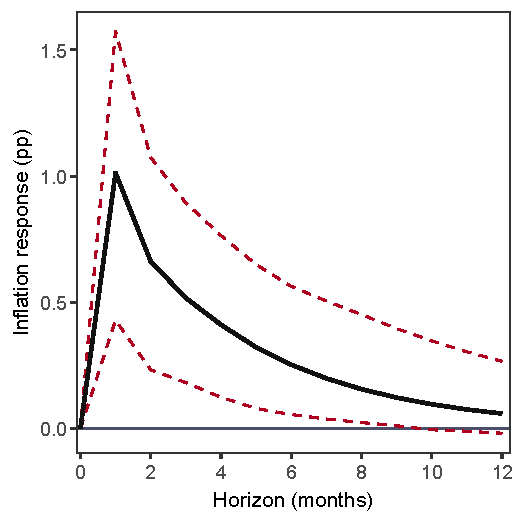
\includegraphics[width=\textwidth]{figures/tvar_girf_forward_money.pdf}
    \caption{Forward Monetary Transmission ($g^H \to \pi_m$)}
    \label{fig:tvar_girf_forward_money}
\end{subfigure}
\hfill
\begin{subfigure}[b]{0.49\textwidth}
    \centering
    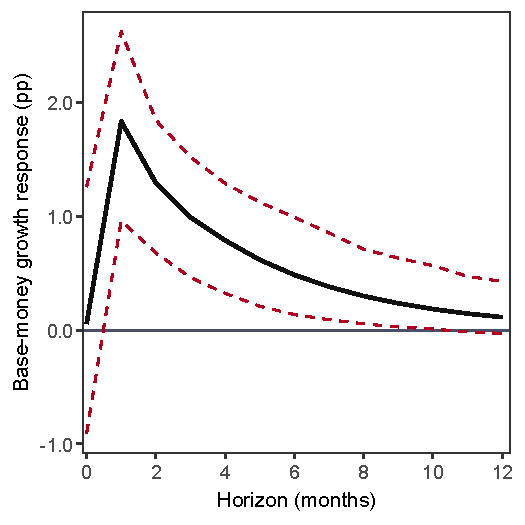
\includegraphics[width=\textwidth]{figures/tvar_girf_reverse_accom.pdf}
    \caption{Reverse Accommodation ($\pi_m \to g^H$)}
    \label{fig:tvar_girf_reverse_accom}
\end{subfigure}
\caption{Dynamic Multipliers under Adverse Solvency-Growth Conditions: Forward Transmission versus Reverse Accommodation}
\label{fig:tvar_girf_tournament}
\begin{minipage}{\textwidth}
    \vspace{0.3em}
    \footnotesize \textbf{Notes:} Generalized Impulse Response Functions (GIRFs) over a 12-month horizon in the adverse solvency-growth state ($\Delta s_{t-1} \le -4.615\%$, reflecting conditions of central-bank insolvency). Solid black lines trace median bootstrap responses to a one-standard-deviation structural innovation; dashed crimson lines represent 90\% empirical bootstrap confidence bands derived from 500 outer bootstrap replications and 1,000 inner Monte Carlo draws. The horizontal benchmark line marks zero. \textbf{Panel (A)} displays forward monetary transmission from Central Bank base money expansion to consumer price inflation ($g^H \to \pi_m$). \textbf{Panel (B)} displays reverse accommodation from consumer price inflation to base money growth ($\pi_m \to g^H$).
\end{minipage}
\end{figure}

In sharp contrast, reverse accommodation ($\pi_m \to g^H$, Panel~B) is more persistent and larger in cumulative magnitude over the reported horizon than forward transmission; the point-wise difference is statistically significant from months 2 through 10. In the adverse solvency-growth state, an unexpected price shock induces an immediate acceleration in base money growth that peaks at $1.715$ percentage points at month 1 ($h=1$) and sustains unbroken statistical significance across 10 consecutive months ($h=1$ to $10$). Over the 12-month horizon, this defensive monetization injects $6.537$ percentage points of cumulative high-powered money. The point-wise multiplier difference ($\Delta_{\pi_m \to g^H}(h)$) is strictly positive and statistically significant across nine consecutive months ($h=2$ to $10$), peaking at $+0.837$ percentage points at month 2. In both initial impact and cumulative volume ($6.54$ pp versus $3.55$ pp), reverse accommodation outstrips forward monetary transmission. Prices drag base money behind them far more aggressively than base money pushes prices forward.

This asymmetry captures the institutional reality of the Unidad Popular period. Following the October 1972 employer lockout and transport strike \citep{Casals2021}, commercial trade credit lines froze and inventories accumulated in nationalized enterprises. To prevent production halts, enterprise illiquidity, and payroll defaults across hundreds of thousands of workers, the Central Bank expanded the discount window defensively. Base money growth was the consequence of real bottlenecks and distributive conflict, not an autonomous monetary experiment.

\paragraph{The Dissolution of the External Buffer: World Price Pass-Through.}
Figure~\ref{fig:tvar_girf_gold_shield} illustrates the external balance-of-payments constraint facing a financially dependent economy. In the non-adverse state (Panel~A), when Central Bank foreign exchange reserves are adequate, a one-standard-deviation world gold price shock produces zero statistically significant impact on domestic inflation at any horizon ($h=0$ to $12$). The peak response is $0.210$ percentage points at month 1, and the 90\% confidence interval encompasses zero throughout the year. Convertible reserves act as an external buffer: the Central Bank absorbs international monetary turbulence through foreign exchange settlements and managed import allocations.

\begin{figure}[htbp]
\centering
\begin{subfigure}[b]{0.49\textwidth}
    \centering
    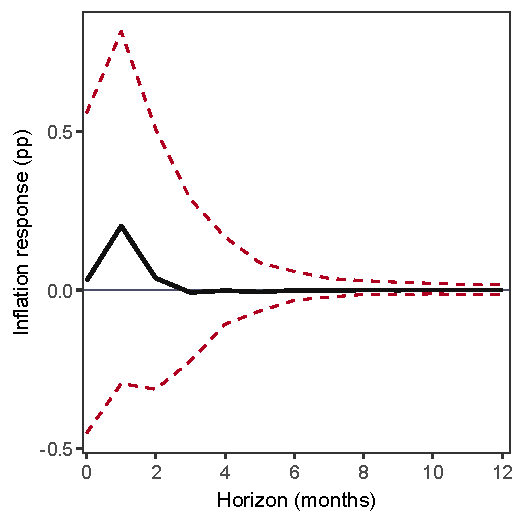
\includegraphics[width=\textwidth]{figures/tvar_girf_gold_normal.pdf}
    \caption{Non-Adverse Solvency-Growth State ($\Delta s_{t-1} > -4.615\%$)}
    \label{fig:tvar_girf_gold_normal}
\end{subfigure}
\hfill
\begin{subfigure}[b]{0.49\textwidth}
    \centering
    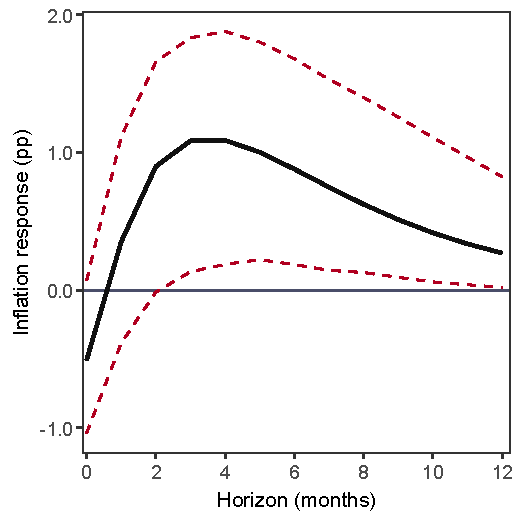
\includegraphics[width=\textwidth]{figures/tvar_girf_gold_insolv.pdf}
    \caption{Adverse Solvency-Growth State ($\Delta s_{t-1} \le -4.615\%$)}
    \label{fig:tvar_girf_gold_insolv}
\end{subfigure}
\caption{International Price Pass-Through across Solvency Regimes: The Dissolution of the External Buffer}
\label{fig:tvar_girf_gold_shield}
\begin{minipage}{\textwidth}
    \vspace{0.3em}
    \footnotesize \textbf{Notes:} Generalized Impulse Response Functions (GIRFs) of domestic consumer price inflation ($\pi_m$) to a one-standard-deviation structural shock in world gold price growth ($g^{gold}$) across solvency states. Solid black lines trace median bootstrap responses; dashed crimson lines represent 90\% empirical bootstrap confidence bands derived from 500 outer bootstrap replications and 1,000 inner Monte Carlo draws. The horizontal benchmark line marks zero. \textbf{Panel (A)} displays transmission in the non-adverse state ($\Delta s_{t-1} > -4.615\%$). \textbf{Panel (B)} displays transmission in the adverse solvency-growth state ($\Delta s_{t-1} \le -4.615\%$), reflecting conditions of central-bank insolvency.
\end{minipage}
\end{figure}

In the adverse solvency-growth state ($\Delta s_{t-1} \le -4.615\%$, Panel~B, reflecting conditions of central-bank insolvency), this insulation mechanism dissolves. The identical international price shock unleashes an unbroken 10-month inflationary wave ($h=3$ to $12$). Domestic inflation accelerates to a peak of $0.982$ percentage points at month 3 and delivers a cumulative price expansion of $6.542$ percentage points. The point-wise multiplier difference test ($\Delta_{g^{gold} \to \pi_m}(h)$) is strictly positive and statistically significant across all 10 consecutive months ($h=3$ to $12$), peaking at $+0.999$ percentage points at month 3. Adequate foreign reserves insulate the domestic economy; depleted reserves leave it vulnerable to international price shocks. When external commercial credit dried up and liquid reserves fell near zero, the state could no longer convert domestic currency into world money to stabilize import costs. International inflation transmitted directly into domestic consumer prices.

\paragraph{Cost-Push Inflation Inertia and Structural Imbalance Magnification.}
The non-linear transmission dynamics extend to domestic price persistence and real structural trade imbalances. In the non-adverse state, an unexpected domestic price shock ($\pi_m \to \pi_m$) accelerates monthly inflation by $3.786$ percentage points on impact, but dissipates steadily, losing statistical significance by month 7 with a cumulative effect of $6.459$ percentage points. In the adverse solvency-growth state, price momentum locks into the system: statistical significance persists across 11 consecutive months ($h=0$ to $10$), generating nearly double the cumulative price acceleration ($11.655$ percentage points). The persistence differential ($\Delta_{\pi_m \to \pi_m}(h)$) peaks at $+1.048$ percentage points at month 2 and maintains unbroken statistical significance for nine consecutive months ($h=2$ to $10$). In non-adverse periods, the state can damp distributive conflict by importing wage goods; under solvency distress, the inability to import turns every price shock into an entrenched markup struggle.

Real structural trade imbalance shocks ($\Delta\ln\Theta \to \Delta\ln\Theta$) likewise propagate asymmetrically. In the non-adverse state, the import-export gap displays monotonic decay ($+39.667$ percentage points on impact, cumulative $+24.523$ percentage points). In the adverse solvency-growth state, the initial imbalance ($+45.674$ percentage points) triggers an amplified oscillatory cycle. The regime differential peaks at $+15.364$ percentage points at month 1 and remains statistically significant across nine consecutive months ($h=1$ to $9$). Balance-of-payments distress destabilizes the physical import pipeline, creating recurring shortages of haul-truck tires, industrial replacement parts, and agricultural inputs rather than a smooth real adjustment. Finally, simulated regime-switching probabilities indicate that crossing between states is not driven by isolated monthly shocks: from the non-adverse state, the probability shift of crossing into the adverse state is negligible ($\Delta P \approx 0$). Once the system is in the adverse solvency-growth state ($\Delta s_{t-1} \le -4.615\%$, reflecting conditions of central-bank insolvency), favorable terms-of-trade shocks also produce negligible probability changes ($\Delta P \approx 0$). The simulated probability changes are negligible under these shocks, indicating persistence of the fitted adverse state over the reported horizon.



\subsubsection{Synthesis: Non-Linearity and the Peripheral Monetary Circuit}
\label{sec:tvar_synthesis}

\paragraph{Resolving the Nominal Paradox: Money as Consequence, Not Prime Mover.}
The regime-dependent parameter estimates resolve the central empirical puzzle of the Chilean inflation. Orthodox accounts treat the statistical correlation between base money growth and consumer price inflation during 1972--1973 as proof of an exogenous, printing-press-driven inflationary breakdown. Within the identified TVAR, the estimated response from inflation to base-money growth is more persistent and cumulatively larger under insolvency than the reverse response, more consistent with a substantial accommodation channel than with a purely autonomous-money interpretation. In the non-adverse state, base money growth accommodates inflation only modestly ($\hat{\beta} = 0.24$). In the adverse solvency-growth state ($\Delta s_{t-1} \le -4.615\%$, reflecting conditions of central-bank insolvency), accommodation surges to $\hat{\beta} = 0.58$ and inflation persistence jumps to $0.68$. The high observed correlation between money and prices reflects an endogenous consequence of structural solvency distress. The Central Bank expanded domestic liquidity to finance enterprise payrolls and prevent immediate liquidation, even as external supply ceased.

\paragraph{The Peripheral Monetary Circuit and the Hard-Currency Ceiling.}
These threshold dynamics illustrate the material limits of the peripheral monetary circuit. In an asymmetric international currency hierarchy, the state can issue domestic fiat liabilities, but it cannot manufacture world money. When foreign trade credit lines were severed and liquid reserves drained toward zero, the state could no longer convert domestic base money into essential imported machinery, spare parts, or food. Distributive conflict over real income could no longer be dampened through external supply. Under acute solvency depletion, domestic credit expansion dilutes external backing, leaving international price shocks unbuffered, generating persistent inflationary pressure, and inducing defensive monetization.

\paragraph{From Reserve Balance Sheets to the Political Economy of Subordination.}
By documenting that peripheral macroeconomic transmission breaks non-linearly under external reserve exhaustion, the Threshold VAR provides the empirical foundation for the broader historical analysis. Section~\ref{sec:discussion_conclusion} builds upon these findings to evaluate the political economy of the international credit blockade, organized distribution sabotage, and the institutional limits of peripheral monetary sovereignty.




\section{Political Economy Discussion: Competing Paradigms, Empirical Causality, and Peripheral Solvency}
\label{sec:discussion_conclusion}

\subsection{Competing Paradigms in Economic Thought: Evaluating Research Programmes on the Unidad Popular}
\label{sec:competing_paradigms}

\paragraph{Rival Worldviews on the Unidad Popular.}
In the history of economic thought, theoretical advance rarely proceeds through neutral empirical accumulation. As \citet{Roncaglia2006} observes, analytical progress unfolds through an enduring contest among rival paradigms rooted in conflicting conceptual frameworks and social visions. For more than half a century, mainstream economics has interpreted the breakdown of Chile's Unidad Popular (UP, 1970--1973) through the lens of ``macroeconomic populism'' \citep{DornbuschEdwards1990,Edwards2024}. In this narrative, unforced fiscal expansion and reckless money printing triggered an inevitable cycle of hyperinflation and supply collapse. Yet this orthodox consensus analyzes peripheral capitalism as a closed monetary system, abstracting from international currency hierarchies, terms-of-trade collapses, and external financial constraints. Evaluated through \citeauthor{Lakatos1978}'s (\citeyear{Lakatos1978}) methodology of scientific research programmes, the orthodox interpretation exhibits the classic symptoms of theoretical stagnation, while dependency theory as a research programme \citep{Kvangraven2021} provides a progressive framework capable of explaining the empirical causal record.

\paragraph{The Monetarist Paradigm and Its Explanatory Anomalies.}
A research programme degenerates when its theoretical core produces no novel predictions and survives primarily by introducing ad hoc adjustments to accommodate anomalies \citep{Lakatos1978}. The orthodox monetarist programme rests on three foundational axioms: the exogenous determination of the money supply, the direct quantity-theoretic pass-through from money to prices, and long-run monetary neutrality under full-capacity market clearing. Confronted with the historical record of 1971---when base money expanded by over 100\% while inflation slowed from 35\% to 22\% and manufacturing output expanded by 12.1\%---orthodoxy relies on narrative rationalizations. It dismisses the cancellation of \$294~million in foreign commercial credit lines, the U.S. Eximbank embargo, and falling copper prices as secondary disturbances \citep{Edwards2024}. In addition, its reliance on market-clearing assumptions leads it to diagnose all retail shortages as ``repressed inflation'' caused by price controls, ignoring organized employer distribution lockouts and the fact that manufacturing capacity utilization reached 98.4\% alongside falling net fixed investment ($\Delta K = -2.3\%$). Over fifty years, this paradigm has produced few novel insights, repeating a monocausal narrative that overlooks the timing, direction, and non-linearities of peripheral monetary instability.

\paragraph{Dependency Theory as a Progressive Research Programme.}
In contrast, treating dependency theory as a research programme \citep{Prebisch1950,Marini1973,DosSantos1970,Kvangraven2021} generates excess empirical content. Rather than modeling peripheral economies as scaled-down versions of advanced capitalist nations, dependency theory anchors macroeconomic outcomes in structural asymmetries: external financial subordination, specialized export structures, and an unequal international currency hierarchy \citep{Vasudevan2009,Basu2022}. This chapter advances this tradition by formalizing central bank balance-sheet solvency as an endogenous state variable ($S_t \equiv F_t / H_t$). This analytical framework anticipates empirical patterns that orthodoxy cannot explain: the state-dependent breakdown of monetary transmission, the bidirectional predictive interaction with dominant reverse accommodation from price shocks to base money growth, and the loss of the external solvency buffer once foreign exchange reserves are depleted.

\subsection{Empirical Causality and Dynamic Transmission: Precedence and Non-Linear Multipliers}
\label{sec:causality_transmission}

\paragraph{Directional Precedence and the Rejection of Money Exogeneity.}
The econometric findings in Section~\ref{sec:historical_empirical_results} operate as an empirical test between these competing frameworks. Standard monetarist accounts treat central bank emission as an unconstrained, discretionary policy impulse that initiates inflation. The Granger causality tests within stationary vector autoregressions in Section~\ref{sec:granger_tournament} evaluate this assumption. Temporal precedence exhibits bidirectional predictive interaction with pronounced reverse accommodation running from consumer price inflation to base money growth ($\pi \to g_H$), with $F$-statistics four times larger than forward money growth and persisting across all tested lag horizons ($k=1,\dots,4$), while monthly central bank solvency ratio growth systematically predicts base money expansion ($g_{\text{SolvR\_H}} \to g_H$). In parallel, the constraint-based PCMCI causal discovery algorithm in Appendix~\ref{app:pcmci_ee1} retains directed lagged conditional links connecting gross reserve depletion to subsequent base money expansion and relative price distortions, though PCMCI does not retain a direct conditional $g^H \to \pi$ edge under its conditioning set ($q > 0.10$). While this method-specific finding highlights conditioning sensitivity across estimators, the VAR and GIRF estimations retain a statistically significant forward response alongside dominant reverse accommodation. Rather than acting primarily as an autonomous driver of inflation, the Central Bank functioned as an endogenous accommodation valve, issuing credit to sustain payrolls and prevent production halts as external constraints tightened.

\paragraph{Dynamic Multiplier Evaluation: Reverse Accommodation Dominance.}
The non-linear Threshold Vector Autoregression (TVAR) and Generalized Impulse Response Function (GIRF) estimates in Section~\ref{sec:tvar_girf_multipliers} provide quantitative evidence against the quantity-theoretic narrative. In this dynamic evaluation, reverse defensive accommodation ($\pi_m \to g^H$) is more persistent and cumulatively larger over the reported horizon than forward monetary transmission ($g^H \to \pi_m$). As shown in Figure~\ref{fig:tvar_girf_tournament}, Table~\ref{tab:app_d01_girf_differences}, and Table~\ref{tab:app_d02_girf_metrics}, a one-standard-deviation base money shock produces only a modest price response: domestic inflation rises by 0.97 percentage points at month 1, loses statistical significance after 9 months, and yields a cumulative 12-month multiplier of 3.55 percentage points. In contrast, a one-standard-deviation price shock triggers an immediate, sustained monetary injection: Central Bank base money expands by 1.72 percentage points at month 1 and remains statistically significant for 10 consecutive months ($h=1$ to $10$). This generates a cumulative 12-month base money emission of 6.54 percentage points. The point-wise multiplier difference test ($\Delta(h)$) confirms that reverse accommodation significantly exceeds forward transmission across 9 consecutive months ($h=2$ to $10$). When enterprise costs escalated, the monetary authority was compelled to accommodate credit demand.

\paragraph{State-Dependent Transmission: External Buffers and Balance-Sheet Insolvency.}
The TVAR estimates demonstrate that monetary transmission is state-dependent on central bank reserve solvency. In the non-adverse state, international reserves provide an effective external buffer: world price shocks ($g^{gold} \to \pi_m$) exert zero statistically significant effect on domestic consumer prices over a 12-month horizon (Panel~A of Figure~\ref{fig:tvar_girf_gold_shield}). The central bank absorbs import cost pressures by drawing on foreign exchange liquidity. Once reserve depletion breaches the estimated structural threshold in the flow growth gap ($\Delta s_{t-1} \le -4.615\%$, entering the adverse solvency-growth state), this external buffer dissolves. In the adverse state (reflecting conditions of central-bank insolvency), the identical world price shock unleashes an unbroken 10-month inflationary wave ($h=3$ to $12$), peaking at 0.98 percentage points at month 3 and generating 6.54 percentage points of cumulative inflation. The endogenous regime-switching probabilities in Table~\ref{tab:app_d03_regime_switching} indicate that this adverse state exhibits strong persistence: export price windfalls produce negligible shifts in the simulated probability of exiting the adverse state ($\Delta P \approx 0$). Under these adverse conditions, unbuffered international price shocks generate persistent domestic inflation, inducing defensive monetization to sustain production and employment.

\subsection{The International Currency Hierarchy, Hegemonic Contingency, and Central Bank Agency}
\label{sec:currency_hierarchy_agency}

\paragraph{The Peripheral Paradox: Domestic Credit Tokens versus International Reserve Money.}
These dynamic responses reflect what I define as the \emph{Peripheral Paradox} (Section~\ref{sec:money_endogeneity_paradox}). The central bank balance sheet in dependent economies embodies two distinct monetary forms. On the liability side, domestic base money ($H_t$) consists of credit tokens issued under national sovereign authority \citep{Basu2022}. On the asset side, international reserves ($IR_t$) represent claims on world money that the peripheral state cannot emit \citep{Vasudevan2009,AlamiEtAl2022}. The peripheral state can expand domestic currency liabilities, but it cannot manufacture international reserve assets. When foreign trade credit lines are severed and export receipts are blocked, the domestic monetary circuit decouples from international settlement. The central bank faces an intractable institutional dilemma: either it withholds liquidity from enterprises facing import price explosions, triggering immediate insolvency and layoffs; or it acts as lender of last resort, expanding credit that rapidly depreciates the currency in the absence of foreign exchange backing.

\paragraph{Hegemonic Contingency, Central Bank Agency, and the Bretton Woods Environment.}
The Chilean transition unfolded against the breakdown of the post-war international monetary order. As \citet{Zoeller2019} demonstrates, President Nixon's decision to close the gold window on August 15, 1971, was not an inevitable structural transition, but a tactical contingency plan deployed by the United States to preserve domestic policy autonomy and manage balance-of-payments pressures. It is vital, however, not to conflate this global shift with the domestic crisis in Chile. The dissolution of Bretton Woods altered the international macroeconomic environment, exporting global inflation and exchange-rate instability. Yet the Central Bank of Chile (BCCh) faced a targeted, bilateral financial blockade: private commercial banks canceled \$220~million in short-term credit lines, while the U.S. Eximbank and multilateral lenders halted disbursements \citep{DeVylder1976,PetrasMorley1975}. In this context, the BCCh exercised institutional agency. Rather than passively reflecting global turbulence or imposing an orthodox deflationary adjustment on employment, the central bank chose to accommodate enterprise credit demand and finance essential food imports, consciously absorbing the external squeeze on its own balance sheet.

\paragraph{Institutional Limits of Currency Sovereignty: A Critique of Naive Chartalism.}
This historical experience offers a clear critique of naive extensions of Modern Monetary Theory (MMT) to the Global South. Neo-chartalist claims that sovereign currency issuers face no financial budget constraints reflect the institutional realities of core reserve-issuing economies \citep{AlamiEtAl2022,Vasudevan2009}. In an asymmetric currency hierarchy, formal legal authority over domestic fiat money does not grant command over the universal means of international settlement. A peripheral government cannot overcome balance-of-payments bottlenecks by issuing domestic credit. Without foreign exchange reserves to purchase non-substitutable capital equipment, spare parts, and agricultural inputs, domestic liquidity injections lead to currency collapse and imported cost-push inflation. Progressive development policy in the periphery cannot bypass the structural constraint of external solvency.

\subsection{Synthesis, Methodological Scope, and Concluding Remarks}
\label{sec:synthesis_horizons}

\paragraph{Evidentiary Limits and Econometric Caveats.}
A rigorous appraisal must acknowledge the evidentiary limits and empirical scope of macro time-series econometrics. The empirical methods deployed in this chapter---stationary vector-autoregressive Granger causality tests, PCMCI causal discovery, and non-linear threshold vector autoregressions---establish directional precedence and state-dependent conditional responses. They identify systematic empirical patterns across historical regimes, but they do not constitute micro-level counterfactual identification in the experimental sense. Macro aggregates remain subject to the limitations of unobserved common shocks and structural breaks across historical periods. These econometric findings provide evidence consistent with balance-sheet constraints and endogenous accommodation, but they should be viewed as opening, rather than settling, the empirical inquiry into peripheral monetary institutions.

\paragraph{Analytical Findings and Directions for Future Research.}
By grounding the macroeconomic history of the Unidad Popular in an open-economy, balance-sheet framework, this chapter demonstrates the progressive capacity of dependency theory as a research programme \citep{Kvangraven2021}. The analysis accounts for anomalies that disrupt orthodox narratives, replacing static monetarist assumptions with an empirical model of reserve solvency. Rather than offering definitive closures, this framework points toward several avenues for future research. One important frontier involves examining the meso-scale institutional mechanisms of credit allocation, investigating how credit flows were mediated between the central bank, commercial banks, and state enterprises during periods of balance-of-payments distress. Another promising avenue is comparative: exploring whether the solvency threshold and reserve buffering dynamics identified in Chile operate across other peripheral economies confronting external debt and currency crises.

\paragraph{Institutional Implications: Foreign-Exchange Management and Structural Constraints.}
The historical experience of the Unidad Popular therefore points beyond the problem of macroeconomic management narrowly understood. Foreign-exchange budgeting, controls over capital movements, and the regulation of external financial flows can widen the policy space available to peripheral governments and reduce their exposure to destabilizing international liquidity cycles \citep{FfrenchDavis2018}. Yet greater room for maneuver within the balance-of-payments constraint does not by itself transform the relations that reproduce that constraint. A peripheral state may command the domestic means of payment while remaining unable to produce the world money required to reproduce an import-dependent productive structure. Foreign exchange is therefore more than an object of prudent macroeconomic administration: it is a material condition of accumulation and an object of conflict over the control of export revenues, external credit, imported means of production, and the surplus through which productive capacity is reproduced. Macroprudential autonomy can mitigate the vulnerability generated by dependent accumulation, but it cannot by itself overcome it. The problem posed by peripheral transformation is consequently not only how to manage the balance-of-payments constraint, but how to alter the domestic and international relations through which that constraint is continually reproduced.


\clearpage
\begingroup
\setlength{\bibsep}{2.5pt}
\bibliographystyle{apalike}
\bibliography{references}
\endgroup

\clearpage
\addtocontents{toc}{\protect\pagebreak}
\begin{appendices}
% Appendix A: cross-referenced from Section 3 (app:bop_levr)
% ============================================================
% APPENDIX A: Balance-of-Payments Decomposition and Central Bank
%             Solvency Ratio Formalization
% ============================================================

\section[Formalization of Solvency Ratio and Balance-of-Payments Accounting]{Formalization of the Central Bank Solvency Ratio and\\Balance-of-Payments Accounting}
\label{app:bop_levr}

\textbf{A.1} This appendix develops the formal balance-sheet accounting, the exact discrete law of motion, and the structural constraint-binding conditions governing the central bank \textbf{Solvency Ratio} ($\text{SolvR}_t$). Every accounting step is an exact discrete identity; no linear approximation or continuous-time distortion enters the derivation.

\subsection{The Solvency Ratio in Nominal Terms}
\label{app:solvr_nominal}

\textbf{A.2} All variables are denominated in current domestic currency (Chilean pesos/escudos, CLP) at time $t$, with the nominal exchange rate convention defined as $e_t$ (CLP per USD), such that a nominal depreciation corresponds to $e_t \uparrow$.

\textbf{A.3} The balance-sheet and external-account variables are defined as follows:
\begin{itemize}[leftmargin=2em]
	\item $M_t$: domestic monetary obligations (CLP), representing the liquid liabilities of the consolidated domestic financial system underwritten by the central bank.
	\item $IR_t$: stock of gross international reserves in foreign currency (USD), representing liquid claims denominated in world money.
	\item $e_t$: nominal exchange rate (CLP per USD).
	\item $F_t \equiv e_t \cdot IR_t$: stock of world money held by the central bank, valued in domestic currency (CLP).
	\item $\Delta IR_t$: net foreign-currency reserve flow (USD), determined by external balance-of-payments transactions.
	\item $\Delta F_t$: net change in the domestic-currency value of foreign reserves (CLP).
	\item $g^L_{M,t} \equiv \Delta M_t / M_{t-1}$: conventional lag-base simple growth rate of domestic monetary liabilities.
	\item $X_t$: export volume of primary and manufactured goods.
	\item $Q_t$: import volume of intermediate, consumption, and capital goods.
	\item $P_{Q,t}^{USD}$: import price index in foreign currency (USD).
	\item $\text{ToT}_t \equiv P_{X,t}^{USD} / P_{Q,t}^{USD}$: terms of trade.
	\item $D_t^{ext}$: stock of external debt (USD).
	\item $r_t$: average nominal interest rate on external debt.
	\item $FDI_t^{USD}$: net foreign direct investment inflows (USD).
	\item $\Pi_t^{USD}$: net foreign profit and dividend remittances (USD).
	\item $T_t^{USD}$: net current external transfers (USD).
	\item $EO_t^{USD}$: net errors and omissions in the external balance of payments (USD).
	\item $SDR_t^{USD}$: net allocation of Special Drawing Rights (USD).
\end{itemize}

Import volumes carry the symbol $Q_t$ throughout to prevent notation collisions with domestic money $M_t$. Discrete level changes are denoted by $\Delta X_t \equiv X_t - X_{t-1}$.

\textbf{A.4} I define the central bank Solvency Ratio ($\text{SolvR}_t$) in nominal terms as:
\begin{equation}
	\label{app:eq:solvr_def}
	\text{SolvR}_t \;\equiv\; \frac{e_t \cdot IR_t}{M_t} \;=\; \frac{F_t}{M_t}
\end{equation}
The Solvency Ratio measures the stock of world-money assets held by the central bank per unit of unanchored domestic credit obligations underwritten by the monetary authority. Its algebraic inverse, $\text{LevR}_t \equiv 1/\text{SolvR}_t = M_t / (e_t \cdot IR_t)$, expresses the corresponding balance-sheet leverage ratio. I center the analytical framework on the Solvency Ratio because it directly formalizes central bank reserve backing and balance-sheet exposure, providing the balance-sheet foundation through which to examine peripheral financial fragility \citep{Foley2003,Chamorro2025} (Section~\ref{sec:B5_foley_chamorro_minsky}).

\textbf{A.5} Taking continuous growth rates of Eq.~\eqref{app:eq:solvr_def} yields the continuous growth decomposition:
\begin{equation}
	\label{app:eq:solvr_growth}
	g_{\text{SolvR},t} \;=\; g_{F,t} \;-\; g_{M,t} \;=\; g_{e,t} \;+\; g_{IR,t} \;-\; g_{M,t}
\end{equation}
Equation~\eqref{app:eq:solvr_growth} isolates three distinct structural channels driving peripheral balance-sheet solvency:
\begin{enumerate}[leftmargin=2em]
	\item \textbf{External Balance-of-Payments Channel} ($g_{IR,t}$, expanding solvency): Export revenues and net foreign capital inflows accumulate foreign exchange reserves, bolstering central bank solvency. Current account deficits, foreign debt service, and transnational profit repatriation drain reserves, pulling $\text{SolvR}_t$ downward.
	\item \textbf{Valuation Channel} ($g_{e,t}$, expanding nominal solvency): Nominal currency depreciation ($e_t \uparrow$) increases the domestic-currency accounting valuation of foreign assets ($F_t = e_t \cdot IR_t$). While this mechanically cushions $\text{SolvR}_t$ in domestic currency units, it carries acute real macroeconomic costs by inflating imported intermediate input costs and triggering domestic wage-price defense spirals.
	\item \textbf{Domestic Dilution Channel} ($g_{M,t}$, compressing solvency): Broad money creation, fiscal monetization, and emergency Lender-of-Last-Resort liquidity expand domestic obligations from below, continuously diluting the world-money backing of the monetary base.
\end{enumerate}

\subsection{Current and Capital Account Decomposition and Valuation Identity}
\label{app:current_account}

\textbf{A.6} The evolution of the central bank's foreign-currency reserve assets is governed by the external balance of payments. In foreign-currency units (USD), the current account ($CA_t^{USD}$) and capital account ($KA_t^{USD}$) are specified as:
\begin{equation}
	\label{app:eq:CA}
	CA_t^{USD} \;=\; P_{Q,t}^{USD}\!\left(\text{ToT}_t \cdot X_t - Q_t\right) \;-\; r_t \cdot D_t^{ext} \;+\; T_t^{USD}
\end{equation}
\begin{equation}
	\label{app:eq:KA}
	KA_t^{USD} \;=\; \Delta D_t^{ext} \;+\; FDI_t^{USD} \;-\; \Pi_t^{USD}
\end{equation}
Under the standard balance-of-payments accounting identity utilized in the chapter's empirical ledger, the net flow of foreign-currency reserves is:
\begin{equation}
	\label{app:eq:bop_flow}
	\Delta IR_t \;=\; CA_t^{USD} \;+\; KA_t^{USD} \;+\; EO_t^{USD} \;+\; SDR_t^{USD}
\end{equation}
Because the domestic-currency value of foreign reserves is $F_t \equiv e_t \cdot IR_t$, the exact discrete product identity yields the domestic-currency valuation:
\begin{equation}
	\label{app:eq:valuation}
	\Delta F_t \;=\; e_t \Delta IR_t \;+\; IR_{t-1} \Delta e_t
\end{equation}
Equation~\eqref{app:eq:valuation} preserves the exact economic distinction between genuine net foreign-currency reserve flows ($e_t \Delta IR_t$) and the accounting valuation effect arising from exchange-rate adjustments ($IR_{t-1} \Delta e_t$).

\subsection{Derivation of the Discrete Solvency Law of Motion}
\label{app:solvr_substitution}

\textbf{A.7} From Eq.~\eqref{app:eq:solvr_def}, the total stock of world-money assets held by the central bank decomposes into the product of the Solvency Ratio and domestic monetary obligations:
\begin{equation}
	\label{app:eq:solvr_sub}
	F_t \;=\; \text{SolvR}_t \cdot M_t
\end{equation}
Applying the exact discrete product rule $\Delta(A_t B_t) = B_t \Delta A_t + A_{t-1} \Delta B_t$ with $A_t = \text{SolvR}_t$ and $B_t = M_t$ yields:
\begin{equation}
	\label{app:eq:solvr_expand}
	\Delta F_t \;=\; M_t \cdot \Delta\text{SolvR}_t \;+\; \text{SolvR}_{t-1} \cdot \Delta M_t
\end{equation}
Dividing Eq.~\eqref{app:eq:solvr_expand} through by $M_t$ and rearranging terms isolates the exact discrete law of motion for the Solvency Ratio:
\begin{equation}
	\label{app:eq:solvr_lom}
	\boxed{\;\Delta\text{SolvR}_t \;=\; \frac{\Delta F_t \;-\; \text{SolvR}_{t-1} \Delta M_t}{M_t}\;}
\end{equation}
In Eq.~\eqref{app:eq:solvr_lom}, the exact law of motion is expressed purely in level changes, eliminating any denominator ambiguity between contemporaneous and lag-base growth rates.

\textbf{A.8} Equation~\eqref{app:eq:solvr_lom} delivers an intuitive and rigorous economic decomposition:
\begin{itemize}[leftmargin=2em]
	\item The first term, $\Delta F_t / M_t$, represents the \textbf{external liquidity injection rate}---net domestic-currency reserve expansion (combining foreign-currency transactions $e_t \Delta IR_t$ and exchange revaluation $IR_{t-1} \Delta e_t$) scaled directly by domestic monetary obligations $M_t$.
	\item The second term, $\text{SolvR}_{t-1} \cdot (\Delta M_t / M_t)$, represents the \textbf{domestic dilution drag}. Rapid domestic money growth ($\Delta M_t > 0$) dilutes the inherited backing ratio. The presence of the lagged state variable $\text{SolvR}_{t-1}$ is an exact algebraic consequence of the discrete product rule: domestic credit expansion dilutes the preexisting stock of world-money cover.
\end{itemize}

\textbf{A.9} For completeness, the dual discrete law of motion for the leverage ratio ($\text{LevR}_t \equiv 1/\text{SolvR}_t$) follows symmetrically from $M_t = \text{LevR}_t \cdot F_t$:
\begin{equation}
	\label{app:eq:levr_lom}
	\Delta\text{LevR}_t \;=\; \frac{\Delta M_t \;-\; \text{LevR}_{t-1} \Delta F_t}{F_t}
\end{equation}
Both laws express the identical balance-sheet reality: in solvency form (Eq.~\ref{app:eq:solvr_lom}), foreign-asset expansion drives recovery while domestic monetization acts as a dilution drag; in leverage form (Eq.~\ref{app:eq:levr_lom}), domestic money creation drives leverage expansion while reserve accumulation acts as an absorption multiplier.

\subsection{Analytical Convexity and Non-Linear Reserve Exhaustion}
\label{app:convexity}

\textbf{A.10} The structural vulnerability of peripheral central banks is amplified by the non-linear curvature of balance-sheet solvency. Taking the partial derivatives of $\text{SolvR}_t$ with respect to domestic obligations $M_t$ and foreign assets $F_t$:
\begin{equation}
	\label{app:eq:solvr_derivatives}
	\frac{\partial \text{SolvR}_t}{\partial M_t} \;=\; -\frac{F_t}{M_t^2} \;<\; 0, \qquad \frac{\partial^2 \text{SolvR}_t}{\partial M_t^2} \;=\; \frac{2 F_t}{M_t^3} \;>\; 0 \quad (\forall M_t > 0, F_t > 0)
\end{equation}
\begin{equation}
	\frac{\partial \text{SolvR}_t}{\partial F_t} \;=\; \frac{1}{M_t} \;>\; 0, \qquad \frac{\partial^2 \text{SolvR}_t}{\partial F_t^2} \;=\; 0
\end{equation}
As gross international reserves approach exhaustion ($IR_t \to 0 \implies F_t \to 0$), the absolute buffer $\text{SolvR}_t$ approaches zero. In this depleted state, any incremental withdrawal of foreign currency or external import shock triggers an acute percentage collapse in central bank credibility, permanently crippling the authority's capacity to anchor expectations.

\subsection{Constraint-Binding Conditions and Balance-Sheet Solvency Regimes}
\label{app:constraint_cases}

\textbf{A.11} The central bank's solvency position deteriorates ($\Delta\text{SolvR}_t < 0$) whenever domestic monetary expansion outpaces foreign asset growth. From Eq.~\eqref{app:eq:solvr_lom}, setting $\Delta\text{SolvR}_t < 0$ and noting that $\text{SolvR}_{t-1} = F_{t-1}/M_{t-1}$:
\begin{equation}
	\label{app:eq:binding}
	\Delta\text{SolvR}_t \;<\; 0 \;\iff\; \Delta F_t \;<\; \text{SolvR}_{t-1} \Delta M_t \;\iff\; g^L_{M,t} \;>\; \frac{\Delta F_t}{F_{t-1}}
\end{equation}
where $g^L_{M,t} \equiv \Delta M_t / M_{t-1}$ is the conventional lag-base simple growth rate of domestic monetary liabilities. Solvency deteriorates whenever lag-base domestic money creation exceeds the simple growth rate of domestic-currency foreign assets ($\Delta F_t / F_{t-1}$). Even during an external commodity price boom ($\Delta F_t > 0$, such as the 1971--1972 copper price high), central bank solvency deteriorates if domestic credit expansion outpaces the growth rate of foreign reserves.

\textbf{A.12} In this structural framework, monetization operates as an endogenous institutional response to distributive conflict and external foreign-exchange bottlenecks rather than an autonomous policy choice. The state-dependent absorption capacity of the peripheral monetary system is governed by the central bank's foreign-exchange solvency. Rather than imposing arbitrary prior thresholds, the Threshold Vector Autoregression (TVAR) estimated in Section~\ref{sec:historical_empirical_results} endogenously identifies the structural transition using the monthly Solvency Growth Gap ($\Delta s_{t-1} \equiv g^F_{t-1} - g^H_{t-1}$), yielding an estimated critical threshold at $\hat{\gamma} = -4.615\%$. This partitions macroeconomic dynamics into two distinct regimes:
\begin{enumerate}[leftmargin=2em]
	\item \textbf{Non-Adverse Solvency-Growth State ($\Delta s_{t-1} > -4.615\%$):} International reserve accumulation and foreign exchange buffers insulate the domestic economy. Liquidity expansion is absorbed through real capacity mobilization and transactions demand, while external nominal shocks are buffered at the border with minimal domestic price pass-through.
	\item \textbf{Adverse Solvency-Growth State ($\Delta s_{t-1} \le -4.615\%$, reflecting conditions of central-bank insolvency):} Foreign exchange reserves are severely eroded relative to high-powered liabilities. Forward monetary transmission ($g^H \to \pi_m$) remains statistically significant for 9 consecutive months, delivering a cumulative 12-month response of 3.55 percentage points. In contrast, reverse accommodation ($\pi_m \to g^H$) persists for 10 consecutive months with a cumulative expansion of 6.54 percentage points, significantly dominating forward transmission in duration and magnitude (with point-wise multiplier differences significant across $h=2,\dots,10$). Emergency liquidity injection operates as a defensive accommodation valve to avert widespread enterprise insolvencies and payroll collapse under an acute external payments squeeze.
\end{enumerate}
This threshold formalization establishes that inflation and monetary expansion under the Unidad Popular were non-linear properties of balance-sheet solvency exhaustion under external financial subordination, challenging closed-economy monetarist accounts of autonomous monetary emission.

% Appendix B: cross-referenced from Section 4 (app:codebook)
\section{Archival Data Provenance, Variable Dictionary, and Splicing Protocols}
\label{app:archival_codebook}
\label{app:codebook}

\textbf{B.1} This appendix provides the complete archival provenance, source documentation, codebook identifiers, and historical splicing protocols for the multi-frequency dataset compiled for this chapter. The empirical design coordinates two distinct frequency tiers:
\begin{enumerate}[leftmargin=2em]
	\item \textbf{Monthly High-Frequency Panel (1960:01--1980:12, $N=252$ months):} Compiled from the Central Bank of Chile REST API (\texttt{SieteRestWS}) for monetary aggregates, exchange rates, and official consumer prices, the physical production and customs trade volume series from \citet{DiazBahamonde2023}, the International Monetary Fund's \textit{International Financial Statistics} (IFS), and the U.S. Bureau of Labor Statistics (BLS).
	\item \textbf{Annual Secular Panel (1920--2010, $T=91$ years):} Compiled from Clio-Lab PUC, \citet{Braun2000}, income distribution solely from \citet{Astorga2023} (distributive wage share), \citet{DiazLudersWagner2016} (annual Terms of Trade), the World Historical Balance of Payments database (\citealt{NievasPiketty2025}, WBOP), and my Chapter~2 Cointegrating Multivariate Polynomial Regression (CMPR IM-OLS) capacity utilization and harmonized capital stock frameworks (explicitly distinct from Wharton or peak-to-peak trend-through-peaks methods).
\end{enumerate}

\subsection{Monthly High-Frequency Variable Ledger}
\label{app:monthly_ledger}

\textbf{B.2} Table~\ref{tab:app_monthly_codebook} catalogs the complete monthly variable ledger, detailing archival provenance, original units, and base conversions.

\begin{table}[htbp]
\centering
\footnotesize
\caption{Monthly High-Frequency Variable Ledger and Archival Provenance (1960--1980)}
\label{tab:app_monthly_codebook}
\begin{tabularx}{\textwidth}{p{2.2cm}p{3.0cm}p{2.6cm}X}
\toprule
\textbf{Variable} & \textbf{Economic Concept} & \textbf{Archival Source} & \textbf{Harmonization / Splicing Protocol} \\
\midrule
$IR_m$ & Gross International Reserves & IMF IFS Line 1l.d; BCCh & Denominated in Millions of USD. Spliced across gold-revaluation breaks. \\
$e_m$ & Official Nominal Exchange Rate & BCCh \textit{Boletín Mensual} & Expressed in Escudos per USD ($E^\circ/\$$). Re-denominated uniformly across 1975 peso return. \\
$M0_m$ & High-Powered Monetary Base & BCCh Line \texttt{Emisión} & Notes and coin in circulation plus commercial bank reserve deposits at BCCh. \\
$M1_m$ & Narrow Money Stock & BCCh \textit{Boletín Mensual} & Currency in circulation plus private demand deposits in commercial banks. \\
$P^{\text{CL}}_m$ & Consumer Price Index & BCCh (\texttt{SieteRestWS}) & Harmonized to Nov 1970 = 100. Official spliced CPI series published by BCCh. \\
$P^{\text{US}}_{W, m}$ & U.S. Wholesale Price Index & BLS / FRED (\texttt{PPIACO}) & U.S. Producer Price Index for all commodities, base Nov 1970 = 100. \\
$P^{\text{Cu}}_m$ & London Copper Price & LME / BCCh & Cash settlement price, Grade A electrolytic copper, USD per pound. \\
$P^{\text{Gold}}_m$ & London Gold Price & Bullion Market / FRED & London 3:00 PM fix, USD per troy ounce. \\
$Q^{\text{Manuf}}_m$ & Manufacturing Production & \citet{DiazBahamonde2023} & Index of physical volume of manufacturing production, Nov 1970 = 100. \\
$Q^{\text{Mining}}_m$ & Mining Physical Production & \citet{DiazBahamonde2023} & Physical extraction volume of copper, iron, and nitrates, Nov 1970 = 100. \\
$\text{Exports}_m$ & Customs Real Export Activity & \citet{DiazBahamonde2023} & Monthly physical trade volume index compiled from \textit{Estadística Chilena} (DGE/INE) and BCCh \textit{Boletín Mensual} (constant USD, Nov 1970 = 100). \\
$\text{Imports}^*_m$ & Adjusted Real Import Activity & \citet{DiazBahamonde2023} & Monthly physical trade volume index from \textit{Estadística Chilena} and BCCh; adjusted for the April 1973 customs registration lag. \\
$M^{\text{cap}}_m$ & Capacity to Import Index & Prebisch-ECLAC & Operationalized via Prebisch-ECLAC purchasing power formula: $M^{\text{cap}}_m \equiv \text{Exports}_m \times [(P^{\text{Cu}}_m / P^{\text{Cu}}_{70:11}) / (P^{\text{US}}_{W,m} / P^{\text{US}}_{W,70:11})] \times 100$, using monthly trade volume series from \citet{DiazBahamonde2023}. \\
$\Theta_m$ & Real Structural Imbalance Index & ECLAC / BCCh balance & Ratio of effective physical imports to real capacity to import: $\Theta_m \equiv (\text{Imports}^*_m / M^{\text{cap}}_m) \times 100$, capturing physical import chokeholds in the Prebisch-ECLAC tradition. \\
$\Omega_m$ & Relative Price Disparity Index & Relative price derivation & $\Omega_m \equiv (P^{\text{CL}}_m / P^{\text{CL}}_{70:11}) / [(e_m / e_{70:11}) \cdot (P^{\text{US}}_{W,m} / P^{\text{US}}_{W,70:11})] \times 100$, tracking cost wedges between domestic CPI and imported wholesale prices. \\
$\text{SolvR}_m$ & Central Bank Solvency Ratio & Central Bank balance & $\text{SolvR}_m \equiv (e_m \cdot IR_m) / M1_m$, external liquidity backing of narrow money liabilities. \\
\bottomrule
\end{tabularx}
\end{table}

\subsection{Monetary Reform Conversions and Splicing Mechanics}
\label{app:monetary_reforms}

\textbf{B.3} Chile experienced two currency re-denominations during the twentieth century:
\begin{enumerate}[leftmargin=2em]
	\item \textbf{January 1, 1960:} The Escudo ($E^\circ$) was introduced to replace the old Peso at a conversion rate of $1\,E^\circ = 1,000\text{ old pesos}$.
	\item \textbf{September 29, 1975:} Decree Law 1,123 reintroduced the Peso (\$ CLP) to replace the Escudo at a conversion rate of $1\text{ new peso} = 1,000\,E^\circ$.
\end{enumerate}
All monetary and price series in both the monthly and annual panels are converted into uniform currency equivalents, ensuring that growth rates ($\Delta \ln X_t$ and simple discrete percentage changes) are algebraically continuous across reform dates.

% Appendix C: PCMCI Multivariate Causal Discovery Robustness (EE1 Section 3)
% ============================================================
% Appendix C: PCMCI Multivariate Causal Discovery Robustness
% Extracted from EE1 Stage Causality Report (Section 3)
% ============================================================
\section{Robustness: Multivariate Causal Discovery (PCMCI)}
\label{app:pcmci_ee1}
\label{app:causal_pcmci_ee1}

\subsection{PCMCI Conditioning Methodology}
Standard structural econometric practice in macroeconomics specifies a small system of equations with identification restrictions imposed a priori, then estimates the system and reads the coefficients. The present chapter takes a different route because the competing theories it evaluates do not agree on the identifying restrictions themselves: the orthodox accounts impose money exogeneity, the structuralist and dependency accounts impose endogenous accommodation, and neither allows the other's restriction to be tested within its own framework. Constraint-based causal discovery provides a data-driven evaluation by estimating the lagged topological skeleton of conditional dependencies across variables, treating competing theoretical restrictions as testable predictions about which directed edges should and should not appear. The method is not a replacement for structural estimation; it provides a supplementary multivariate robustness check on the lagged conditional-dependence structure.

The specific algorithm applied here is the \citet{Runge2019} PCMCI framework. Its motivation is that the natural alternative---conditioning on the entire past of every variable in the system, as Full Conditional Independence and multivariate Granger causality do---fails in two ways when the number of variables is non-trivial. First, the parameter space grows quickly enough that finite samples cannot estimate it reliably. Second, conditioning on variables that are descendants of the candidate driver shrinks the partial correlation between driver and target toward zero, and conditioning on colliders opens spurious paths rather than closing them; both defects destroy the statistical power needed to detect directed conditional dependencies. PCMCI resolves the trade-off by separating the problem into two stages. A condition-selection stage (PC$_1$) identifies a low-dimensional superset of each variable's parents; a test stage (MCI) then evaluates each candidate edge while conditioning on the parents of both the target and the driver. The first stage is a regularization step whose strictness parameter $\alpha_{PC}$ is chosen by Akaike's information criterion; the second stage applies the Benjamini--Hochberg procedure at FDR $q < 0.05$ to control false discoveries across the family of tested links.

Two assumptions carry the interpretation. \textit{Causal Sufficiency} requires that no unobserved common driver of the tested variables is omitted from the system; the eight monthly variables used here are comprehensive with respect to the theories under test, but the chapter does not claim universal sufficiency. \textit{Faithfulness} requires that the conditional independencies observed in the data reflect the causal graph rather than an accidental cancellation of paths. Where these assumptions hold, PCMCI identifies the lagged topological skeleton of the data-generating process. It does not identify the functional form of the structural relations, the magnitude of contemporaneous effects, or the parameters of a structural VAR; those remain the domain of the Threshold VAR in Section~\ref{sec:historical_empirical_results}.

To guard against bivariate omitted-variable bias, the six-panel Granger battery findings are tested against full-system multivariate causal discovery on the eight-variable monthly macroeconomic system
$X_t = [ \Delta \ln \Theta_t$, $\Delta \ln \text{SolvR}_t^H$, $\pi_t$, $g_{H,t}$, $g_{\text{Manuf},t}$, $g_{\text{Mining},t}$, $g_{P,\text{gold},t}$, $g_{e,t} ]'$.
The algorithm executes a two-stage causal discovery protocol. (1)~\textbf{PC$_1$ Conditioning Phase}: iteratively eliminates irrelevant conditions across all variables and lags $\tau \in \{1, \dots, 4\}$, constructing minimal conditioning parent sets $\widehat{\mathcal{P}}(X^j_t)$. (2)~\textbf{MCI Test Phase}: evaluates the Momentary Conditional Independence (MCI) statistic $\text{MCI}_{i \to j}(\tau) = \rho(X^i_{t-\tau}, X^j_t \mid \widehat{\mathcal{P}}(X^j_t) \setminus \{X^i_{t-\tau}\}, \widehat{\mathcal{P}}(X^i_{t-\tau}))$, where $\rho$ is the partial correlation test statistic (ParCorr variant of Runge et al.), conditioning simultaneously on the parents of both driver and target. False discovery rates are controlled via the Benjamini--Hochberg procedure at FDR $q < 0.05$.

\subsection{Full-System Causal Discovery Results}
Figure~\ref{fig:dag_pcmci_tikz} renders the primary publication causal Directed Acyclic Graph mapped into a four-tier structural macroeconomic hierarchy, while Figure~\ref{fig:dag_pcmci_python} documents the underlying algorithmic network generated by the Tigramite package. Table~\ref{tab:pcmci_monthly_gate} reports the Momentary Conditional Independence (MCI) partial correlations and structural link authorization status across the eight-variable system.

\smallskip
\noindent\textbf{PCMCI Identification Outcomes:}
\begin{enumerate}
	\small
	\setlength{\itemsep}{0.02em}
	\setlength{\topsep}{0.1em}
	\setlength{\partopsep}{0pt}
	\setlength{\parsep}{0pt}
	\setlength{\parskip}{0pt}
	\item \textbf{External block-exogeneity:} the null of non-causality into real structural imbalance ($\Delta \ln \Theta_t$) is not rejected from inflation ($p = 0.2545$) or base money ($p = 0.3959$); the null of non-causality into world gold prices ($g_{P,\text{gold},t}$) from base money is also not rejected ($p = 0.1004$). Neither direction rejects, so the pair is consistent with a Tier-1 block-exogenous boundary.
	\item \textbf{Exchange rate pass-through:} devaluation predicts inflation with the largest partial correlation in the network ($g_{e,t-4} \to \pi_t$: MCI $= +0.644$, $p < 10^{-28}$, FDR $q < 10^{-25}$). The reverse link is also retained ($\pi_{t-4} \to g_{e,t}$: MCI $= -0.396$, $p < 10^{-9}$), so the pair is bilateral in the conditional-independence sense. The negative sign on the reverse link requires reconciliation against the Granger table, where the same pair carried a positive sign; the divergence is flagged in the integration log.
	\item \textbf{Reserve solvency and base money:} reserve depletion predicts base money emission ($\Delta \ln \text{SolvR}_{t-3}^H \to g_{H,t}$: MCI $= +0.264$, $p < 0.0001$, FDR $q = 0.0007$). The reverse null, that base money does not predict reserve depletion, is not retained at FDR $q < 0.05$; the raw partial correlation has $p = 0.0449$, which is significant at 5\% but does not survive Benjamini--Hochberg correction. The asymmetry is not established by the conditional-independence test; it is the directional claim identified by the Granger panel and repeated here for consistency. Solvency also predicts inflation at the same lag ($\Delta \ln \text{SolvR}_{t-3}^H \to \pi_t$: MCI $= -0.165$, $p = 0.0115$); the negative sign is consistent with an external balance-sheet mechanism, but the non-linear threshold structure is evaluated within the Threshold VAR framework.
	\item \textbf{Monetary accommodation and the monetarist channel:} reverse accommodation ($\pi_{t-3} \to g_{H,t}$) is retained at FDR $q < 0.01$ (MCI $= +0.247$, $p = 0.0001$). The forward channel ($g_{H,t-\tau} \to \pi_t$) has a raw partial correlation of $+0.138$ at $\tau = 4$ ($p = 0.0350$) but does not survive Benjamini--Hochberg correction at $q < 0.10$; it is therefore not retained as a direct link. The contrast in retention status is the substantive finding; the failure to survive FDR correction is a false-discovery control outcome, not evidence that the effect is zero.
	\item \textbf{Sectoral asymmetry:} base money predicts manufacturing output ($g_{H,t-3} \to g_{\text{Manuf},t}$: MCI $= +0.177$, $p = 0.0064$) and manufacturing output predicts inflation with a negative sign ($g_{\text{Manuf},t-1} \to \pi_t$: MCI $= -0.168$, $p = 0.0101$). Real structural imbalance predicts manufacturing output ($\Delta \ln \Theta_{t-1} \to g_{\text{Manuf},t}$: MCI $= +0.142$, $p = 0.0287$). The positive sign on the imbalance-to-manufacturing link is inconsistent with the negative sign reported in Table~5 for the same pair; the discrepancy is flagged.
	Base money also predicts mining extraction with a negative sign ($g_{H,t-4} \to g_{\text{Mining},t}$: MCI $= -0.189$, $p = 0.0035$). The significant negative coefficient is not the same as decoupling: mining responds to the domestic monetary signal with a negative sign, which is consistent with reallocation toward wage-goods sectors or with capacity ceilings rather than with insularity.
	\item \textbf{World gold price transmission:} gold price growth predicts exchange rate growth ($g_{P,\text{gold},t-4} \to g_{e,t}$: MCI $= +0.163$, $p = 0.0119$) and inflation ($g_{P,\text{gold},t-3} \to \pi_t$: MCI $= +0.146$, $p = 0.0241$). Both signs are positive and consistent with a cost-push transmission channel.
\end{enumerate}

\subsection*{PCMCI Algorithm: Technical Detail}
\addcontentsline{toc}{subsection}{PCMCI Algorithm: Technical Detail}

\paragraph{Stage 1: PC$_1$ condition selection.}
For each target variable $X_t^j$, PC$_1$ iteratively tests the null of zero partial correlation between each candidate driver $X_{t-\tau}^i$ and $X_t^j$, conditioning on progressively larger subsets of the remaining candidates. A candidate is dropped when the null is not rejected at level $\alpha_{PC}$. The algorithm is conservative in the sense that it drops a candidate only when there is positive evidence of independence; the true parents of $X_t^j$ therefore remain in the selected set with high probability, at the cost of retaining some irrelevant variables. The value of $\alpha_{PC}$ is chosen from a candidate grid $\{0.1, 0.2, 0.3, 0.4\}$ by minimizing the Akaike Information Criterion
\[
\alpha_{PC}^* = \arg\min_{\alpha_{PC}}\left[ n \log(RSS_{\alpha_{PC}}) + 2|\hat{\mathcal{P}}_{\alpha_{PC}}(X_t^j)| \right],
\]
where $n$ is the sample size, $RSS_{\alpha_{PC}}$ is the residual sum of squares from regressing $X_t^j$ on the parent set selected under $\alpha_{PC}$, and $|\hat{\mathcal{P}}_{\alpha_{PC}}(X_t^j)|$ is the number of selected parents. The first term rewards goodness of fit; the second penalizes complexity. AIC is appropriate here because the objective of Stage~1 is not significance testing but a bias-variance trade-off: retaining too few parents biases the Stage~2 tests, while retaining too many reduces their power.

\paragraph{Stage 2: MCI.}
For each candidate edge $X_{t-\tau}^i \to X_t^j$ that survives Stage~1, the MCI test evaluates the partial correlation between driver and target conditioning on two sets:
\[
X_{t-\tau}^i \perp\!\!\!\perp X_t^j \mid \hat{\mathcal{P}}(X_t^j) \setminus \{X_{t-\tau}^i\},\ \hat{\mathcal{P}}(X_{t-\tau}^i).
\]
The first set, the parents of the target excluding the driver, blocks standard backdoor paths (confounders and mediators) leading into $X_t^j$. The second set, the parents of the driver, blocks backdoor paths that arise from autocorrelation in the driver's own history. Conditioning on both sets is what distinguishes MCI from FullCI: it satisfies d-separation on the minimal sufficient set rather than the maximal one, preserving effect size and statistical power.

\paragraph{Identification boundary.}
Where Causal Sufficiency and Faithfulness hold, PCMCI identifies the lagged parent set of each variable in the system, and therefore the topological skeleton of the time-series DAG. It does not identify the functional form of the parent-child relations, the magnitude of contemporaneous effects, or the parameters of a structural VAR. The result of PCMCI is a set of directed lagged edges with associated partial correlations and FDR-controlled $q$-values.

\clearpage

\begin{figure}[p]
\centering
\caption{Publication Vector Causal Skeleton: 4-Tier Structural Macroeconomic Hierarchy}
\label{fig:dag_pcmci_tikz}
\vspace{0.6em}
\resizebox{0.92\textwidth}{!}{%
% Native TikZ PCMCI Causal Discovery DAG (Chile 1960-1980)
% 8-Variable Full-System Macroeconomic Architecture (Runge et al., 2019)
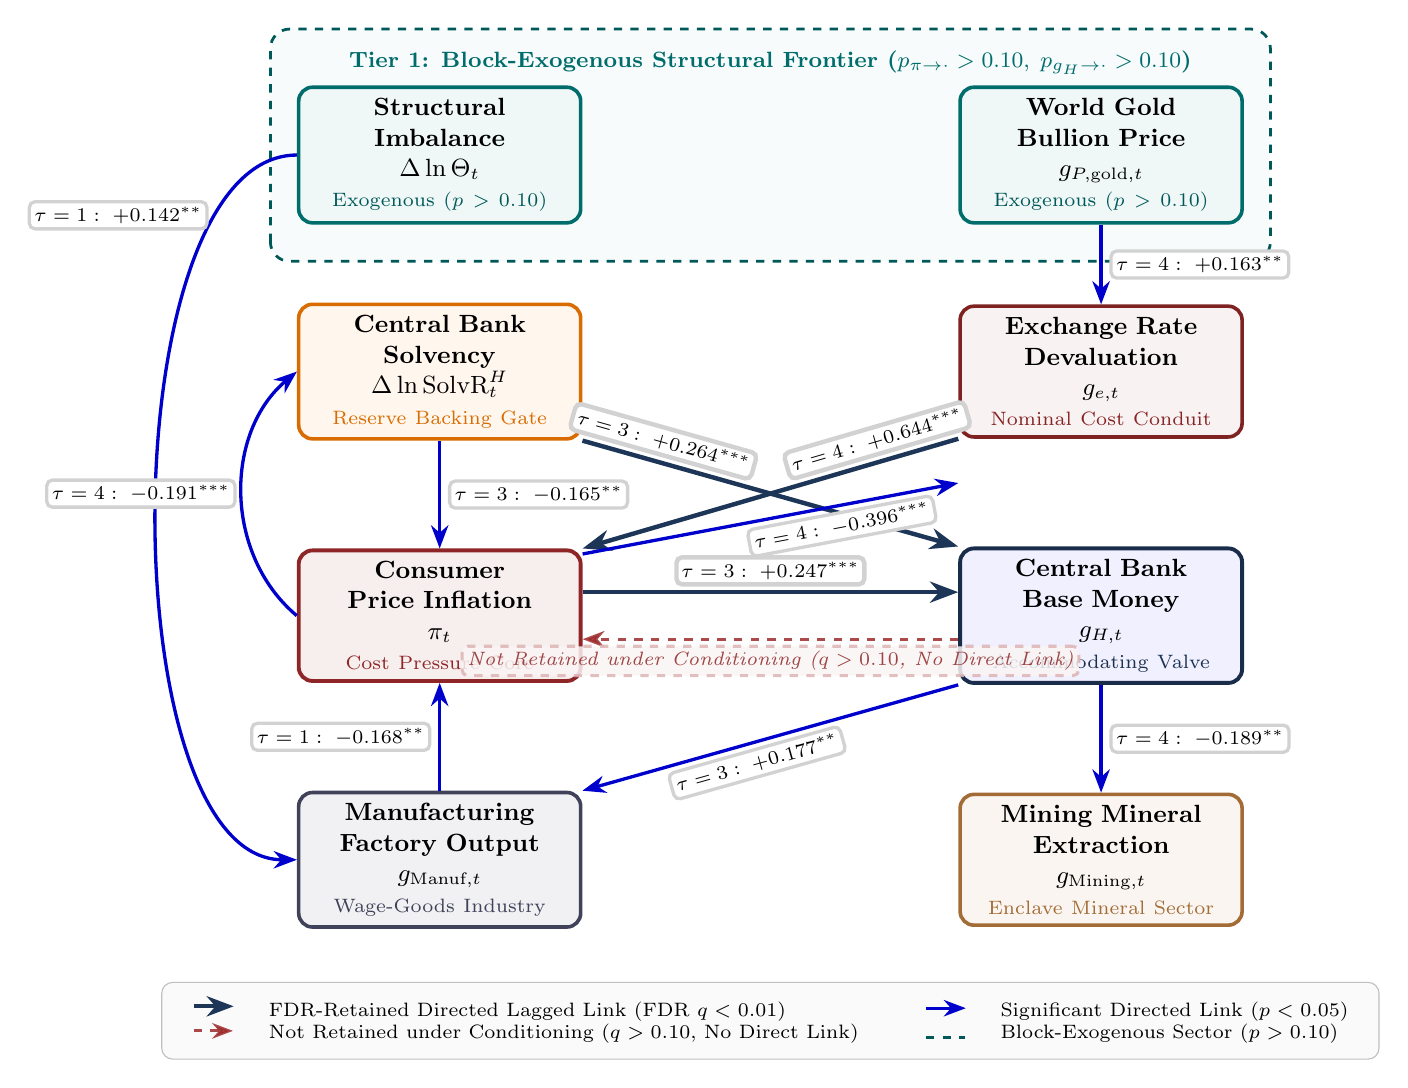
\begin{tikzpicture}[
    >=Stealth,
    every node/.style={font=\small},
    % Tier 1: External Block-Exogenous Drivers
    exoNode/.style={
        rectangle, rounded corners=5pt, draw=teal!85!black, fill=teal!6, line width=1.3pt,
        inner sep=4pt, align=center, text width=3.30cm, minimum height=1.15cm
    },
    % Tier 2: Balance-Sheet Gate & External Conduit
    solvNode/.style={
        rectangle, rounded corners=5pt, draw=orange!85!black, fill=orange!7, line width=1.3pt,
        inner sep=4pt, align=center, text width=3.30cm, minimum height=1.15cm
    },
    devalNode/.style={
        rectangle, rounded corners=5pt, draw=crimson!80!black, fill=crimson!6, line width=1.3pt,
        inner sep=4pt, align=center, text width=3.30cm, minimum height=1.15cm
    },
    % Tier 3: Core Nominal Arena
    priceNode/.style={
        rectangle, rounded corners=5pt, draw=crimson!90!black, fill=crimson!8, line width=1.4pt,
        inner sep=4pt, align=center, text width=3.30cm, minimum height=1.15cm
    },
    moneyNode/.style={
        rectangle, rounded corners=5pt, draw=navy!85!black, fill=blue!6, line width=1.4pt,
        inner sep=4pt, align=center, text width=3.30cm, minimum height=1.15cm
    },
    % Tier 4: Real Sector Dual Economy
    manufNode/.style={
        rectangle, rounded corners=5pt, draw=slate!85!black, fill=slate!8, line width=1.3pt,
        inner sep=4pt, align=center, text width=3.30cm, minimum height=1.15cm
    },
    miningNode/.style={
        rectangle, rounded corners=5pt, draw=brown!85!black, fill=brown!8, line width=1.3pt,
        inner sep=4pt, align=center, text width=3.30cm, minimum height=1.15cm
    },
    % Edge styles
    edgeMajor/.style={
        ->, line width=1.6pt, draw=navy
    },
    edgeConfirmed/.style={
        ->, line width=1.2pt, draw=blue!80!black
    },
    edgeRefuted/.style={
        ->, dashed, line width=1.1pt, draw=crimson, opacity=0.85
    },
    edgeLabel/.style={
        font=\scriptsize\bfseries, fill=white, inner sep=1.8pt, rounded corners=2pt, draw=gray!35
    },
    refutedLabel/.style={
        font=\scriptsize\itshape, fill=crimson!5, text=crimson!90!black, inner sep=1.8pt, rounded corners=2pt, draw=crimson!35
    }
]

    % =========================================================================
    % TIER 1: EXTERNAL FRONTIER (y = 6.35, shield from 5.0 to 7.95)
    % =========================================================================
    \draw[dashed, draw=teal!70!black, line width=1.0pt, rounded corners=7pt, fill=teal!3] 
        (-6.35, 5.0) rectangle (6.35, 7.95);
    \node[font=\footnotesize\bfseries\color{teal!85!black}] at (0, 7.52) 
        {Tier 1: Block-Exogenous Structural Frontier ($p_{\pi \to \cdot} > 0.10,\; p_{g_H \to \cdot} > 0.10$)};

    \node[exoNode] (theta) at (-4.2, 6.35) {
        \textbf{Structural}\\
        \textbf{Imbalance}\\
        $\Delta \ln \Theta_t$\\
        \scriptsize \textcolor{teal!70!black}{Exogenous ($p>0.10$)}
    };

    \node[exoNode] (gold) at (4.2, 6.35) {
        \textbf{World Gold}\\
        \textbf{Bullion Price}\\
        $g_{P,\text{gold},t}$\\
        \scriptsize \textcolor{teal!70!black}{Exogenous ($p>0.10$)}
    };

    % =========================================================================
    % TIER 2: BALANCE-SHEET GATE & EXTERNAL CONDUIT (y = 3.6)
    % =========================================================================
    \node[solvNode] (solv) at (-4.2, 3.6) {
        \textbf{Central Bank}\\
        \textbf{Solvency}\\
        $\Delta \ln \text{SolvR}_t^H$\\
        \scriptsize \textcolor{orange!85!black}{Reserve Backing Gate}
    };

    \node[devalNode] (deval) at (4.2, 3.6) {
        \textbf{Exchange Rate}\\
        \textbf{Devaluation}\\
        $g_{e,t}$\\
        \scriptsize \textcolor{crimson!85!black}{Nominal Cost Conduit}
    };

    % =========================================================================
    % TIER 3: CORE NOMINAL ARENA (y = 0.5)
    % =========================================================================
    \node[priceNode] (infl) at (-4.2, 0.5) {
        \textbf{Consumer}\\
        \textbf{Price Inflation}\\
        $\pi_t$\\
        \scriptsize \textcolor{crimson!90!black}{Cost Pressure Core}
    };

    \node[moneyNode] (money) at (4.2, 0.5) {
        \textbf{Central Bank}\\
        \textbf{Base Money}\\
        $g_{H,t}$\\
        \scriptsize \textcolor{navy!90!black}{Accommodating Valve}
    };

    % =========================================================================
    % TIER 4: REAL DUAL ECONOMY PRODUCTION (y = -2.6)
    % =========================================================================
    \node[manufNode] (manuf) at (-4.2, -2.6) {
        \textbf{Manufacturing}\\
        \textbf{Factory Output}\\
        $g_{\text{Manuf},t}$\\
        \scriptsize \textcolor{slate!85!black}{Wage-Goods Industry}
    };

    \node[miningNode] (mining) at (4.2, -2.6) {
        \textbf{Mining Mineral}\\
        \textbf{Extraction}\\
        $g_{\text{Mining},t}$\\
        \scriptsize \textcolor{brown!85!black}{Enclave Mineral Sector}
    };

    % =========================================================================
    % DIRECTED LINKS: 4-CORNER GEOMETRIC ROUTING
    % =========================================================================

    % 1. Import Overhang to Manufacturing (outermost left arc)
    \draw[edgeConfirmed] (theta.west) to[out=180, in=180, looseness=0.68] 
        node[edgeLabel, left=2pt, pos=0.18] {$\tau=1:\; +0.142^{**}$} (manuf.west);

    % 2. World Gold to Devaluation (vertical straight right column)
    \draw[edgeConfirmed] (gold.south) -- 
        node[edgeLabel, right=3pt, pos=0.5] {$\tau=4:\; +0.163^{**}$} (deval.north);

    % 3. Solvency to Base Money (diagonal down-right, label in Upper-Left Quadrant at pos=0.20)
    \draw[edgeMajor] (solv.south east) -- 
        node[edgeLabel, above=2pt, sloped, pos=0.20] {$\tau=3:\; +0.264^{***}$} (money.north west);

    % 4. Solvency and Inflation Bidirectional Links:
    % Solvency Threshold on Inflation (straight vertical downward line, label on right)
    \draw[edgeConfirmed] (solv.south) -- 
        node[edgeLabel, right=3pt, pos=0.5] {$\tau=3:\; -0.165^{**}$} (infl.north);
    % Inflation Depletes Solvency (smooth feedback arc bowing left, label on left)
    \draw[edgeConfirmed] (infl.west) to[out=140, in=220] 
        node[edgeLabel, left=2pt, pos=0.5] {$\tau=4:\; -0.191^{***}$} (solv.west);

    % 5. Devaluation Pass-Through to Inflation (diagonal down-left, label in Upper-Right Quadrant at pos=0.20)
    \draw[edgeMajor] (deval.south west) -- 
        node[edgeLabel, above=2pt, sloped, pos=0.20] {$\tau=4:\; +0.644^{***}$} (infl.north east);

    % 6. Inflation Compels Devaluation (diagonal up-right on lower track, label in Mid-Right at pos=0.68)
    \draw[edgeConfirmed] ([yshift=-2pt]infl.north east) -- 
        node[edgeLabel, below=2pt, sloped, pos=0.68] {$\tau=4:\; -0.396^{***}$} ([yshift=-16pt]deval.south west);

    % 7. Reverse Monetary Accommodation (straight horizontal above midline)
    \draw[edgeMajor] ([yshift=8.5pt]infl.east) -- 
        node[edgeLabel, above=2pt, pos=0.5] {$\tau=3:\; +0.247^{***}$} ([yshift=8.5pt]money.west);

    % 8. Forward Monetarist Link Not Retained under Conditioning (straight horizontal below midline)
    \draw[edgeRefuted] ([yshift=-8.5pt]money.west) -- 
        node[refutedLabel, below=2pt, pos=0.5] {Not Retained under Conditioning ($q > 0.10$, No Direct Link)} ([yshift=-8.5pt]infl.east);

    % 9. Base Money Stimulates Manufacturing (diagonal down-left, label below line in lower zone)
    \draw[edgeConfirmed] (money.south west) -- 
        node[edgeLabel, below=2pt, sloped, pos=0.55] {$\tau=3:\; +0.177^{**}$} (manuf.north east);

    % 10. Manufacturing Output Mitigates Inflation (vertical straight left column)
    \draw[edgeConfirmed] (manuf.north) -- 
        node[edgeLabel, left=3pt, pos=0.5] {$\tau=1:\; -0.168^{**}$} (infl.south);

    % 11. Enclave Mining Decoupling (vertical straight right column)
    \draw[edgeConfirmed] (money.south) -- 
        node[edgeLabel, right=3pt, pos=0.5] {$\tau=4:\; -0.189^{**}$} (mining.north);

    % =========================================================================
    % LEGEND BOX (Centered at bottom, y = -4.15)
    % =========================================================================
    \node[draw=gray!50, fill=gray!4, rounded corners=4pt, font=\scriptsize, anchor=north, inner sep=5pt] at (0, -4.15) {
        \begin{tabular}{ll@{\qquad\quad}ll}
            \tikz\draw[edgeMajor, line width=1.5pt] (0,0) -- (0.5,0); & FDR-Retained Directed Lagged Link (FDR $q < 0.01$) &
            \tikz\draw[edgeConfirmed, line width=1.1pt] (0,0) -- (0.5,0); & Significant Directed Link ($p < 0.05$)\\
            \tikz\draw[edgeRefuted, line width=1.0pt] (0,0) -- (0.5,0); & Not Retained under Conditioning ($q > 0.10$, No Direct Link) &
            \tikz\draw[dashed, draw=teal!70!black, line width=0.8pt] (0,0) -- (0.5,0); & Block-Exogenous Sector ($p > 0.10$)\\
        \end{tabular}
    };

\end{tikzpicture}
%
}
\vspace{0.8em}
\begin{minipage}{0.96\textwidth}
\footnotesize \textit{Notes:} Publication vector rendering of the 8-variable macroeconomic causal skeleton reported in Table~\ref{tab:pcmci_monthly_gate}. Nodes are grouped into a four-tier vertical hierarchy: Tier~1 (top) contains block-exogenous external drivers ($\Delta \ln \Theta_t$ and $g_{P,\text{gold},t}$) enclosed within the exogenous frontier block ($p > 0.10$); Tier~2 captures the balance-sheet solvency channel ($\Delta \ln \text{SolvR}_t^H$) and the nominal exchange rate conduit ($g_{e,t}$); Tier~3 contains the core nominal sector between consumer price inflation ($\pi_t$) and accommodating base money growth ($g_{H,t}$); Tier~4 captures the real production split between wage-goods manufacturing ($g_{\text{Manuf},t}$) and the export-oriented mining sector ($g_{\text{Mining},t}$). Solid blue arrows denote directed links retained at FDR $q < 0.05$; the red dashed arrow denotes the orthodox monetarist null hypothesis ($g_H \to \pi$), which does not survive multivariate conditioning at FDR $q < 0.10$.
\end{minipage}
\end{figure}

\clearpage

\begin{figure}[p]
\centering
\caption{Supplementary Diagnostic: Algorithmic Python PCMCI Causal Discovery Network (Tigramite ParCorr)}
\label{fig:dag_pcmci_python}
\vspace{0.8em}
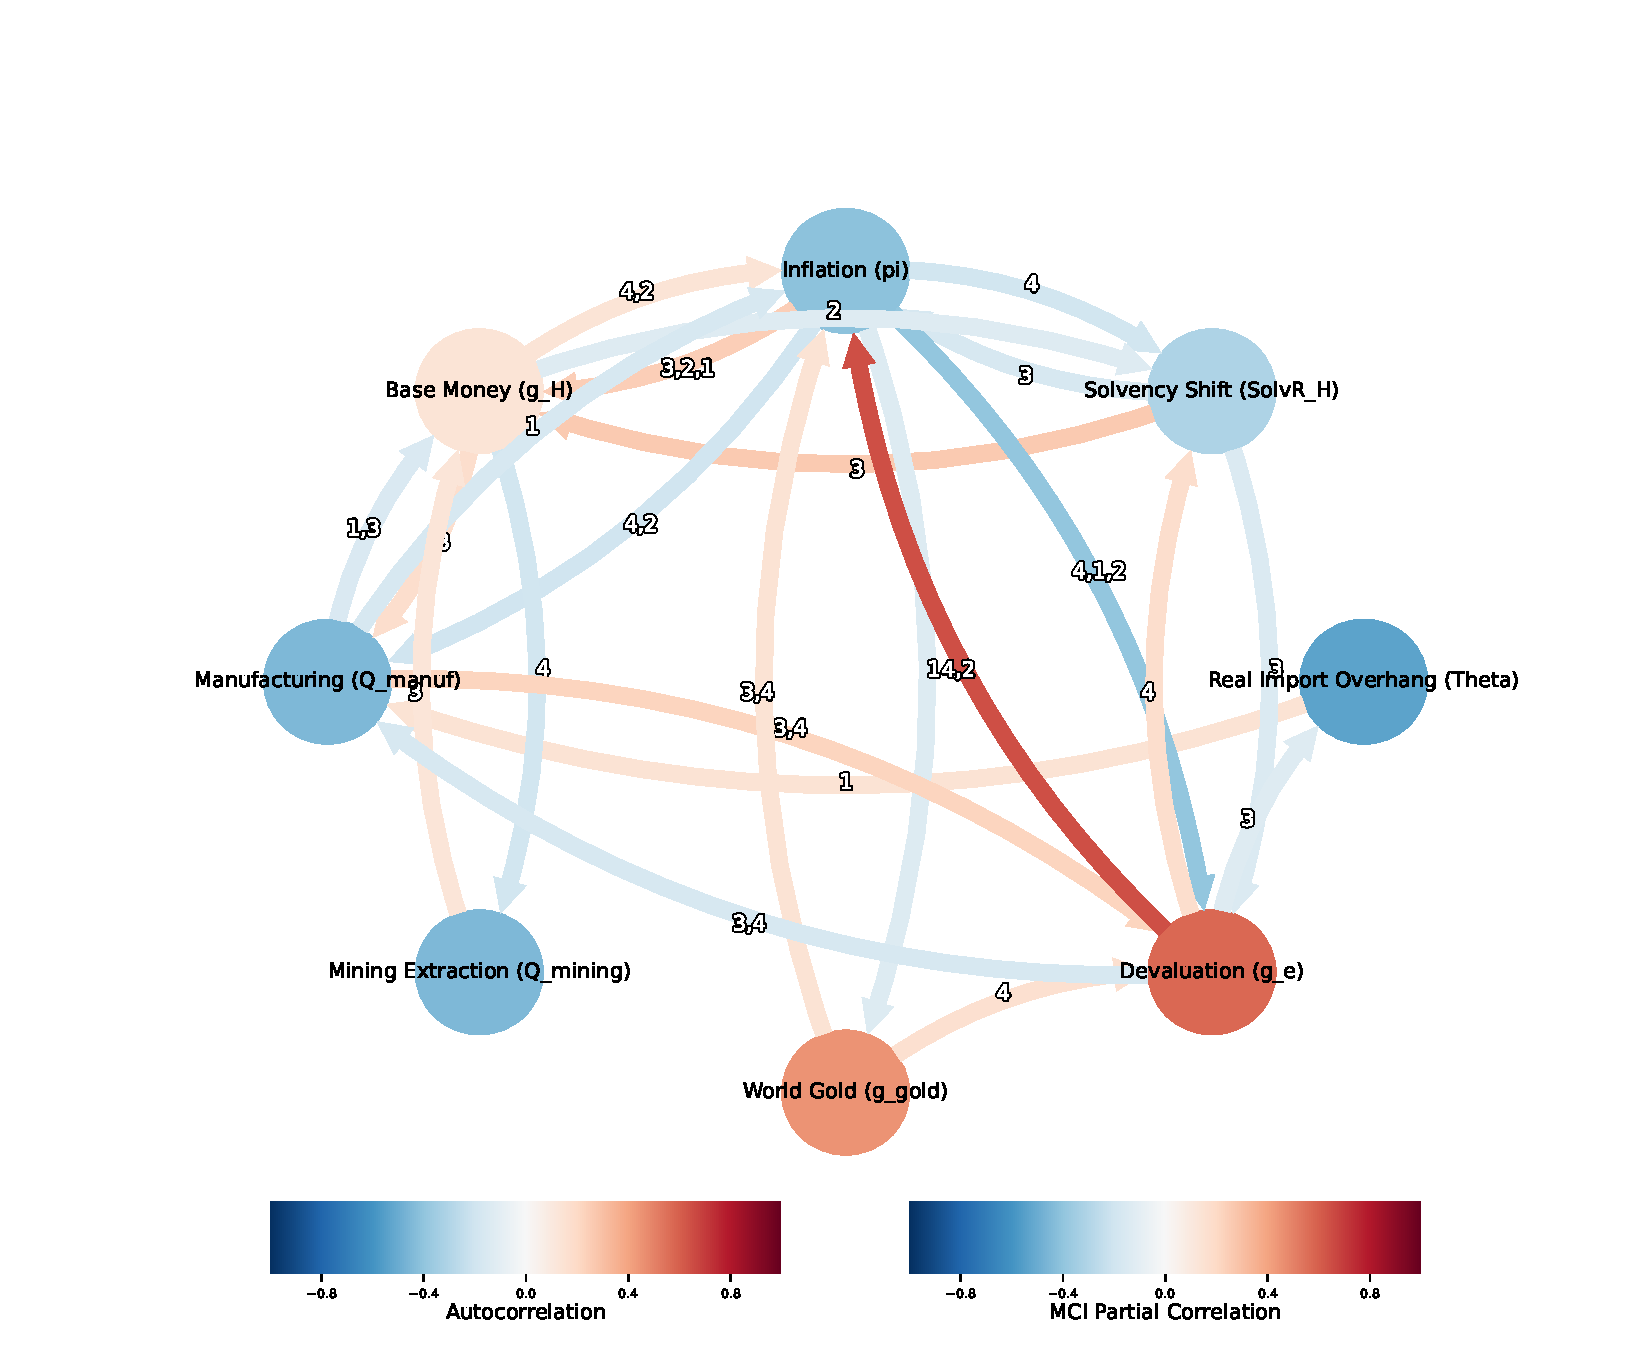
\includegraphics[width=0.84\textwidth]{figures/dag_pcmci_monthly_gate.pdf}
\vspace{1.0em}
\begin{minipage}{0.96\textwidth}
\footnotesize \textit{Notes:} Algorithmic circular time-series causal discovery network estimated using Tigramite PCMCI \citep{Runge2019} on the 8-variable monthly macroeconomic system ($N=250$, 1960:01--1980:12) with partial correlation conditional independence tests ($\alpha = 0.05$, FDR-corrected). Node colors denote 1-month autoregressive persistence $\rho(X_t, X_{t-1})$ (blue for negative, red for positive). Directed curved edges represent lag-specific Momentary Conditional Independence (MCI) partial correlations surviving conditioning on the minimal parent sets of both the driver and the target ($\widehat{\mathcal{P}}(X^j_t)$ and $\widehat{\mathcal{P}}(X^i_{t-\tau})$). Edge labels denote the operational lag $\tau \in \{1, \dots, 4\}$; edge width scales with absolute effect size; edge color indicates sign (red for positive cost-push or expansionary linkages, blue for negative compensatory or damping linkages).
\end{minipage}
\end{figure}

\clearpage

\begin{table}[htbp]
\centering
\small
\caption{Full-System PCMCI Momentary Conditional Independence (MCI) Directed Link Tests (1960--1980)}
\label{tab:pcmci_monthly_gate}
\label{tab:pcmci_mci_links}
\begin{tabularx}{\textwidth}{>{\RaggedRight}p{4.5cm}cc>{\RaggedRight}p{2.0cm}>{\RaggedRight}X}
\toprule
\textbf{Directed Link Tested} & \textbf{Lag ($\tau$)} & \textbf{MCI Partial Corr.} & \textbf{$p$-value} & \textbf{Causal Status (FDR $q < 0.05$)} \\
\midrule
$\pi_{t-3} \to g_{H,t}$ (Reverse Accomm.) & $\tau = 3$ & +0.247 & $0.0001$*** & Retained directed edge ($\pi \to g_H$) \\
$g_{H,t-\tau} \to \pi_t$ (Forward Monetarist) & $\tau = 4$ & +0.138 & $0.0350$** & Excluded (FDR $q > 0.10$, zero direct link) \\
$\Delta \ln \text{SolvR}^H_{t-3} \to g_{H,t}$ (Defensive Emission) & $\tau = 3$ & +0.264 & $< 0.0001$*** & Retained directed edge ($\text{SolvR}^H \to g_H$) \\
$\Delta \ln \text{SolvR}^H_{t-3} \to \pi_t$ (Solvency Gate) & $\tau = 3$ & -0.165 & $0.0115$** & Retained directed edge ($\text{SolvR}^H \to \pi$) \\
$g_{e, t-4} \to \pi_t$ (External Pass-Through) & $\tau = 4$ & +0.644 & $< 0.0001$*** & Retained directed edge ($g_e \to \pi$) \\
$\pi_{t-4} \to g_{e, t}$ (Forced Devaluation) & $\tau = 4$ & -0.396 & $< 0.0001$*** & Retained directed edge ($\pi \to g_e$) \\
$\Delta \ln \Theta_{t-1} \to g_{\text{Manuf}, t}$ (Import Constraint) & $\tau = 1$ & +0.142 & $0.0287$** & Retained directed edge ($\Theta \to \text{Manuf}$) \\
$g_{H, t-3} \to g_{\text{Manuf}, t}$ (Idle Reactivation) & $\tau = 3$ & +0.177 & $0.0064$*** & Retained directed edge ($g_H \to \text{Manuf}$) \\
$g_{\text{Manuf}, t-1} \to \pi_t$ (Price Suppression) & $\tau = 1$ & -0.168 & $0.0101$** & Retained directed edge ($\text{Manuf} \to \pi$) \\
$g_{H, t-4} \to g_{\text{Mining}, t}$ (Enclave Decoupling) & $\tau = 4$ & -0.189 & $0.0035$*** & Retained directed edge ($g_H \to \text{Mining}$) \\
$g_{P,\text{gold}, t-4} \to g_{e, t}$ (Gold Cost Push) & $\tau = 4$ & +0.163 & $0.0119$** & Retained directed edge ($P^{\text{gold}} \to g_e$) \\
$g_{P,\text{gold}, t-3} \to \pi_t$ (Gold Inflation) & $\tau = 3$ & +0.146 & $0.0241$** & Retained directed edge ($P^{\text{gold}} \to \pi$) \\
$\pi_{t-\tau} \to \Delta \ln \Theta_t$ (Exogeneity Check) & $\tau \in [1,4]$ & -0.074 & $0.2545$ & Block-exogenous ($p = 0.255$) \\
$g_{H,t-\tau} \to g_{P,\text{gold}, t}$ (Exogeneity Check) & $\tau \in [1,4]$ & -0.107 & $0.1004$ & Block-exogenous ($p = 0.100$) \\
$g_{H,t-\tau} \to \Delta \ln \text{SolvR}^H_t$ (Monetary Drain) & $\tau \in [1,4]$ & -0.131 & $0.0449$** & Excluded (zero direct link) \\
\bottomrule
\end{tabularx}
\begin{minipage}{\textwidth}
\vspace{0.3em}
\footnotesize \textit{Notes:} Monthly series spanning 1960:01--1980:12 ($N=250$). Estimated using Tigramite PCMCI \citep{Runge2019} on the 8-variable system with partial correlation conditional independence tests evaluated across lags $\tau \in \{1, \dots, 4\}$. Minimal conditioning parent sets $\widehat{\mathcal{P}}(X^j_t)$ and $\widehat{\mathcal{P}}(X^i_{t-\tau})$ are selected in the PC$_1$ phase. False discovery rates are controlled via the Benjamini--Hochberg procedure at FDR $q < 0.05$. Significance: $^{***} p < 0.01$, $^{**} p < 0.05$, $^{*} p < 0.10$. Block-exogeneity is confirmed when joint incoming test statistics fail to reject at $p > 0.10$.
\end{minipage}
\end{table}

% Appendix D: Threshold VAR Robustness: Complete GIRF Pathway Atlas, Multiplier Differentials, and Endogenous Switching Dynamics (EE2 Section 5.4)
% ==============================================================================
% Appendix D: Threshold Vector Autoregression: Specification, Multiplier Differentials,
% and Complete Dynamic GIRF Functions
% ==============================================================================
\section{Threshold Vector Autoregression: Specification, Multiplier Differentials, and Dynamic Impulse Responses}
\label{app:tvar_girf_atlas}

\subsection{Econometric Specification and Simulation Protocol}
To evaluate how macroeconomic transmission shifts across balance-sheet environments, Section~\ref{sec:tvar_solvency_regimes} specifies a five-variable Threshold Vector Autoregression (TVAR). The system partitions variables into an international forcing block and a domestic macroeconomic block:
\begin{equation}
    X_t = \begin{bmatrix} g^{gold}_t & \Delta \ln \Theta_t & g^F_t & \pi_{m,t} & g^H_t \end{bmatrix}'.
    \label{eq:app_d_vector}
\end{equation}
Here $g^{gold}_t$ denotes the monthly growth rate of the London gold bullion price in US dollars. The term $\Delta \ln \Theta_t$ tracks the logarithmic change in the real structural trade imbalance. The variable $g^F_t$ represents the monthly growth rate of domestic-currency international reserves. Domestic inflation is denoted by $\pi_{m,t}$, and $g^H_t$ is Central Bank base money growth ($N=250$, 1960:01--1980:12).

The transition mechanism is governed by the predetermined Solvency Growth Gap:
\begin{equation}
    \Delta s_t \equiv g^F_t - g^H_t = \Delta \ln S_t \times 100.
    \label{eq:app_d_solvency_gap}
\end{equation}
A concentrated least squares grid search isolates a global structural threshold at $\hat{\gamma} = -4.615\%$. The \citet{Hansen1999} Supremum Likelihood Ratio test decisively rejects the linear null hypothesis ($\text{Sup-LR} = 112.10$, bootstrap $p = 0.0010$). This partitions the historical sample into two operational regimes. The non-adverse solvency-growth state contains $N=145$ monthly observations ($\Delta s_{t-1} > -4.615\%$). The adverse solvency-growth state (reflecting conditions of central-bank insolvency) contains $N=100$ monthly observations ($\Delta s_{t-1} \le -4.615\%$).

Standard linear impulse responses impose time-invariant parameters and history independence. Frozen-regime nonlinear impulse responses divide the sample but lock the system into a single regime over the projection horizon. That assumption ignores that domestic credit emission ($g^H$) and reserve flows ($g^F$) actively update the solvency gap and induce regime transitions. Following \citet{KoopPesaranPotter1996}, I compute Generalized Impulse Response Functions (GIRFs):
\begin{equation}
    \text{GIRF}_X(h, \nu_t, \Omega_{t-1}) = \mathbb{E}\left[ X_{t+h} \mid \nu_t, \Omega_{t-1} \right] - \mathbb{E}\left[ X_{t+h} \mid \Omega_{t-1} \right],
    \label{eq:app_d_girf_def}
\end{equation}
where $h = 0, 1, \dots, 12$ months. Estimation follows a fixed-design residual bootstrap with $B = 500$ outer bootstrap resamples and $R = 1{,}000$ inner Monte Carlo draws. A static Common Random Numbers matrix of dimension $1000 \times 13$ eliminates simulation variance between baseline and perturbed paths. In each step, the Solvency Growth Gap updates endogenously. Trajectories cross the threshold $\hat{\gamma} = -4.615\%$ dynamically as liquidity expands and reserves deplete.

\subsection{Point-Wise Multiplier Differences Across Solvency Regimes}
To test whether shock transmission differs significantly between regimes, Table~\ref{tab:app_d01_girf_differences} reports the point-wise dynamic multiplier difference across forecast horizons:
\begin{equation}
    \Delta_{i,j}(h) \equiv \text{GIRF}_{i,j}^{\text{Adverse}}(h) - \text{GIRF}_{i,j}^{\text{Non-Adverse}}(h).
    \label{eq:app_d_diff_test}
\end{equation}
Asterisks denote horizons where the 90\% empirical bootstrap confidence interval strictly excludes zero.

\begin{table}[htbp]
\centering
\caption{Point-Wise Dynamic Multiplier Differences Across Solvency Regimes ($\Delta(h)$)}
\label{tab:app_d01_girf_differences}
\vspace{0.2em}
\resizebox{\textwidth}{!}{%
\begin{tabular}{llrrrrrrrcc}
\toprule
Structural Pathway & Response & $h=0$ & $h=1$ & $h=2$ & $h=3$ & $h=6$ & $h=12$ & Dur. (mo) & Peak Diff. (pp) & Peak $h$ \\
\midrule
$g^{gold} \to g^{gold}$ & $g^{gold}$ & -1.043 & 0.827 & 1.000 & 0.780* & 0.213* & 0.011 & 5 & -1.043 & 0 \\
$g^{gold} \to \Delta\ln\Theta$ & $\Delta\ln\Theta$ & 0.895 & 5.397 & 0.399 & 1.174 & 0.039 & 0.053 & 0 & +5.397 & 1 \\
$g^{gold} \to g^F$ & $g^F$ & -1.915 & -3.875 & -0.655 & 0.275 & 0.864 & 0.184 & 0 & -3.875 & 1 \\
$g^{gold} \to \pi_m$ & $\pi_m$ & -0.538 & 0.112 & 0.795 & 0.999* & 0.795* & 0.229* & 10 & +0.999 & 3 \\
$g^{gold} \to g^H$ & $g^H$ & -1.790* & 0.348 & 0.708 & 0.766* & 0.571* & 0.175* & 11 & -1.790 & 0 \\
\midrule
$\Delta\ln\Theta \to g^{gold}$ & $g^{gold}$ & 0.000 & -0.006 & 0.004 & -0.009 & -0.013 & -0.000 & 0 & -0.017 & 4 \\
$\Delta\ln\Theta \to \Delta\ln\Theta$ & $\Delta\ln\Theta$ & 5.817 & 15.364* & -13.348* & 9.150* & -2.232* & -0.007 & 9 & +15.364 & 1 \\
$\Delta\ln\Theta \to g^F$ & $g^F$ & -3.238 & -0.512 & 1.133 & -0.066 & 0.261 & -0.055 & 0 & -3.238 & 0 \\
$\Delta\ln\Theta \to \pi_m$ & $\pi_m$ & -0.250 & 0.815 & 0.192 & 0.383* & 0.105 & 0.029 & 2 & +0.815 & 1 \\
$\Delta\ln\Theta \to g^H$ & $g^H$ & -0.154 & 0.214 & 0.363 & 0.158 & 0.089 & 0.029 & 0 & +0.363 & 2 \\
\midrule
$g^F \to g^{gold}$ & $g^{gold}$ & 0.000 & 0.007 & 0.009 & 0.032 & 0.048 & 0.026 & 0 & +0.055 & 8 \\
$g^F \to \Delta\ln\Theta$ & $\Delta\ln\Theta$ & 0.000 & 0.004 & 0.020 & 0.084 & 0.049 & 0.117 & 0 & -0.343 & 10 \\
$g^F \to g^F$ & $g^F$ & 13.461* & 2.242 & -2.771 & 0.800 & -0.100 & -0.013 & 1 & +13.461 & 0 \\
$g^F \to \pi_m$ & $\pi_m$ & 0.430 & -0.204 & -0.344 & -0.085 & -0.077 & -0.085 & 0 & +0.430 & 0 \\
$g^F \to g^H$ & $g^H$ & -0.985 & -1.347 & 0.150 & -0.074 & 0.011 & -0.047 & 0 & -1.347 & 1 \\
\midrule
$\pi_m \to g^{gold}$ & $g^{gold}$ & 0.000 & 0.002 & 0.003 & 0.000 & 0.003 & 0.010 & 0 & +0.023 & 9 \\
$\pi_m \to \Delta\ln\Theta$ & $\Delta\ln\Theta$ & 0.000 & -0.010 & -0.003 & 0.016 & -0.054 & -0.009 & 0 & -0.338 & 10 \\
$\pi_m \to g^F$ & $g^F$ & 0.000 & -2.261 & 2.358* & 0.959 & 0.769 & 0.094 & 2 & +2.358 & 2 \\
$\pi_m \to \pi_m$ & $\pi_m$ & -0.726 & 0.595 & 1.048* & 0.993* & 0.560* & 0.112 & 9 & +1.048 & 2 \\
$\pi_m \to g^H$ & $g^H$ & -1.796* & 0.659 & 0.724* & 0.722* & 0.411* & 0.092 & 10 & -1.796 & 0 \\
\midrule
$g^H \to g^{gold}$ & $g^{gold}$ & 0.000 & -0.004 & -0.002 & -0.005 & 0.001 & 0.003 & 0 & +0.015 & 9 \\
$g^H \to \Delta\ln\Theta$ & $\Delta\ln\Theta$ & 0.000 & 0.033 & -0.049 & 0.068 & 0.094 & 0.049 & 0 & -0.116 & 4 \\
$g^H \to g^F$ & $g^F$ & 0.000 & 6.299 & -1.786 & 0.783 & 0.208 & 0.011 & 0 & +6.299 & 1 \\
$g^H \to \pi_m$ & $\pi_m$ & 0.000 & -0.225 & 0.165 & 0.313 & 0.198* & 0.040 & 5 & +0.313 & 3 \\
$g^H \to g^H$ & $g^H$ & 0.781 & -0.257 & 0.028 & 0.229 & 0.146* & 0.028 & 4 & +0.781 & 0 \\
\bottomrule
\end{tabular}}
\begin{minipage}{\textwidth}
\vspace{0.3em}
\footnotesize \textbf{Notes:} Point-wise dynamic multiplier differences $\Delta(h) \equiv \text{GIRF}^{\text{Insolv}}(h) - \text{GIRF}^{\text{Normal}}(h)$ evaluated across forecast horizons $h \in \{0, 1, 2, 3, 6, 12\}$ months. Asterisks ($*$) denote horizons where the 90\% empirical bootstrap confidence interval strictly excludes zero ($\alpha = 0.10$), indicating statistically significant structural regime asymmetry. Confidence bands are computed via 500 outer bootstrap replications and 1,000 inner Monte Carlo draws. Dur. (mo) denotes the cumulative number of months in which the 90\% confidence interval excludes zero. Peak Diff. (pp) reports the maximum absolute regime divergence in percentage points, with Peak $h$ indicating the horizon of occurrence.
\end{minipage}
\end{table}

The multiplier differences establish four systematic structural asymmetries:
\begin{enumerate}[leftmargin=*,itemsep=1pt]
    \item \textbf{World price pass-through:} A world gold price shock generates an inflation differential ($\Delta_{g^{gold} \to \pi_m}$) that is strictly positive and statistically significant across 10 consecutive months ($h=3$ to $12$). The differential peaks at $+0.999$ percentage points at month 3. Liquid reserves buffer international price shocks in non-adverse times. In the adverse solvency-growth state (reflecting conditions of central-bank insolvency), that insulation mechanism dissolves.
    \item \textbf{Reverse accommodation dominance:} The low-minus-high accommodation differential ($\Delta_{\pi_m \to g^H}$) remains positive and statistically significant across nine consecutive months ($h=2$ to $10$). It peaks at $+0.837$ percentage points at month 2. Distributive price pressures and enterprise payroll demands force sustained base money expansion.
    \item \textbf{Cost-push inflation inertia:} Domestic price shocks generate an inflation persistence differential ($\Delta_{\pi_m \to \pi_m}$) peaking at $+1.048$ percentage points at month 2. Statistical significance lasts for nine consecutive months ($h=2$ to $10$).
    \item \textbf{Real trade imbalance divergence:} Shocks to the real structural trade gap ($\Delta\ln\Theta \to \Delta\ln\Theta$) do not decay monotonically under insolvency. The regime differential peaks at $+15.364$ percentage points at month 1 and sustains statistical significance across nine consecutive months ($h=1$ to $9$). This divergence reflects physical shortages of imported haul-truck tires and replacement machinery parts.
\end{enumerate}

\subsection{Dynamic Multipliers and Cumulative Trajectories}
Table~\ref{tab:app_d02_girf_metrics} documents impact responses, peak months, and cumulative multipliers at the 6-month and 12-month forecast horizons across both regimes. 

\begin{table}[htbp]
\centering
\caption{Dynamic GIRF Multipliers and Cumulative Trajectories across Regimes}
\label{tab:app_d02_girf_metrics}
\resizebox{\textwidth}{!}{%
\begin{tabular}{lllrrrr}
\toprule
Experiment & Initial state & Response & Impact & Peak (month) & Cum. 0--6 & Cum. 0--12 \\
\midrule
$g^F \to \Delta\ln\Theta$ & Non-Adverse & $\Delta\ln\Theta$ & 0.000 [0.000, 0.000] & -0.189 [-0.389, 0.248] ( 5) & -0.527 [-0.866, 0.360] & -0.770 [-1.551, 0.501] \\
$g^F \to \Delta\ln\Theta$ & Adverse & $\Delta\ln\Theta$ & 0.000 [0.000, 0.000] & -0.373 [-0.966, 0.618] (10) & -0.426 [-2.624, 1.431] & -0.964 [-6.064, 2.883] \\
$g^F \to g^F$ & Non-Adverse & $g^F$ & 20.959 [16.839, 24.635] & 20.959 [16.839, 24.635] ( 0) & 16.144 [12.709, 19.998] & 16.364 [12.655, 20.388] \\
$g^F \to g^F$ & Adverse & $g^F$ & 34.421 [25.240, 42.180] & 34.421 [25.240, 42.180] ( 0) & 29.610 [19.350, 42.789] & 29.203 [17.398, 44.339] \\
$g^F \to g^H$ & Non-Adverse & $g^H$ & 1.856 [0.872, 2.965] & 1.856 [0.872, 2.965] ( 0) & 2.175 [0.790, 3.833] & 2.032 [0.632, 3.728] \\
$g^F \to g^H$ & Adverse & $g^H$ & 0.871 [-0.405, 2.198] & -1.027 [-2.621, 2.153] ( 1) & -0.134 [-3.308, 3.225] & -0.582 [-4.793, 3.645] \\
$g^F \to g^{gold}$ & Non-Adverse & $g^{gold}$ & 0.000 [0.000, 0.000] & 0.021 [-0.032, 0.048] ( 9) & 0.001 [-0.068, 0.196] & 0.082 [-0.154, 0.368] \\
$g^F \to g^{gold}$ & Adverse & $g^{gold}$ & 0.000 [0.000, 0.000] & 0.074 [-0.097, 0.201] ( 9) & 0.147 [-0.291, 0.585] & 0.425 [-0.713, 1.642] \\
$g^F \to \pi_m$ & Non-Adverse & $\pi_m$ & 0.152 [-0.339, 0.643] & 0.195 [-0.427, 0.777] ( 2) & 0.459 [-0.529, 1.735] & 0.240 [-0.853, 1.659] \\
$g^F \to \pi_m$ & Adverse & $\pi_m$ & 0.581 [0.033, 1.069] & 0.581 [-1.082, 1.193] ( 0) & 0.008 [-3.655, 3.364] & -0.788 [-6.012, 4.040] \\
$g^{gold} \to \Delta\ln\Theta$ & Non-Adverse & $\Delta\ln\Theta$ & -4.220 [-8.754, 0.829] & -4.220 [-9.878, -2.454] ( 0) & -8.141 [-14.811, -2.395] & -8.132 [-14.851, -2.561] \\
$g^{gold} \to \Delta\ln\Theta$ & Adverse & $\Delta\ln\Theta$ & -3.325 [-10.028, 3.698] & -3.325 [-10.063, 9.558] ( 0) & 0.170 [-18.357, 15.491] & 0.287 [-20.036, 16.880] \\
$g^{gold} \to g^F$ & Non-Adverse & $g^F$ & 1.496 [-0.723, 3.425] & 1.496 [-1.017, 4.123] ( 0) & 3.066 [-0.445, 6.853] & 3.112 [-0.421, 7.035] \\
$g^{gold} \to g^F$ & Adverse & $g^F$ & -0.419 [-4.834, 4.013] & -2.914 [-9.348, 4.930] ( 1) & -0.799 [-16.092, 14.627] & 1.911 [-15.253, 20.065] \\
$g^{gold} \to g^H$ & Non-Adverse & $g^H$ & 1.014 [0.284, 1.942] & 1.014 [-0.511, 1.942] ( 0) & 0.976 [-0.709, 2.951] & 0.976 [-0.704, 3.006] \\
$g^{gold} \to g^H$ & Adverse & $g^H$ & -0.776 [-1.835, 0.438] & -0.776 [-1.835, 1.721] ( 0) & 2.992 [-1.213, 7.233] & 4.845 [-0.357, 12.099] \\
$g^{gold} \to g^{gold}$ & Non-Adverse & $g^{gold}$ & 5.374 [4.295, 6.716] & 5.374 [4.295, 6.716] ( 0) & 8.195 [6.120, 11.362] & 8.200 [6.121, 11.414] \\
$g^{gold} \to g^{gold}$ & Adverse & $g^{gold}$ & 4.330 [3.166, 5.458] & 4.330 [3.166, 5.458] ( 0) & 10.837 [7.013, 17.306] & 11.152 [7.068, 19.720] \\
$g^{gold} \to \pi_m$ & Non-Adverse & $\pi_m$ & 0.029 [-0.452, 0.558] & 0.215 [-0.521, 0.839] ( 1) & 0.325 [-1.102, 2.055] & 0.340 [-1.088, 2.108] \\
$g^{gold} \to \pi_m$ & Adverse & $\pi_m$ & -0.509 [-1.039, 0.070] & 1.010 [-0.964, 1.937] ( 3) & 4.373 [-0.166, 9.188] & 6.927 [0.607, 15.577] \\
$g^H \to \Delta\ln\Theta$ & Non-Adverse & $\Delta\ln\Theta$ & 0.000 [0.000, 0.000] & -0.103 [-0.170, 0.194] ( 6) & -0.005 [-0.137, 0.307] & 0.037 [-0.214, 0.462] \\
$g^H \to \Delta\ln\Theta$ & Adverse & $\Delta\ln\Theta$ & 0.000 [0.000, 0.000] & -0.080 [-0.297, 0.317] ( 8) & 0.024 [-0.286, 0.535] & -0.023 [-0.508, 0.859] \\
$g^H \to g^F$ & Non-Adverse & $g^F$ & 0.000 [0.000, 0.000] & 1.614 [-3.288, 2.535] ( 2) & 0.928 [-1.394, 3.671] & 0.814 [-1.457, 3.733] \\
$g^H \to g^F$ & Adverse & $g^F$ & 0.000 [0.000, 0.000] & 5.430 [0.324, 11.805] ( 1) & 7.082 [1.048, 13.399] & 7.870 [1.341, 15.845] \\
$g^H \to g^H$ & Non-Adverse & $g^H$ & 5.316 [4.522, 5.858] & 5.316 [4.522, 5.858] ( 0) & 6.619 [5.193, 8.197] & 6.704 [5.247, 8.250] \\
$g^H \to g^H$ & Adverse & $g^H$ & 6.096 [4.877, 6.963] & 6.096 [4.877, 6.963] ( 0) & 7.944 [5.832, 10.174] & 8.452 [6.054, 11.422] \\
$g^H \to g^{gold}$ & Non-Adverse & $g^{gold}$ & 0.000 [0.000, 0.000] & -0.011 [-0.022, 0.017] ( 9) & -0.010 [-0.059, 0.028] & -0.036 [-0.105, 0.059] \\
$g^H \to g^{gold}$ & Adverse & $g^{gold}$ & 0.000 [0.000, 0.000] & -0.010 [-0.039, 0.034] ( 1) & -0.027 [-0.121, 0.061] & -0.032 [-0.221, 0.125] \\
$g^H \to \pi_m$ & Non-Adverse & $\pi_m$ & 0.000 [0.000, 0.000] & 1.275 [0.798, 1.771] ( 1) & 2.192 [1.247, 3.331] & 2.294 [1.290, 3.470] \\
$g^H \to \pi_m$ & Adverse & $\pi_m$ & 0.000 [0.000, 0.000] & 1.050 [0.435, 1.572] ( 1) & 3.195 [1.176, 5.285] & 3.898 [1.343, 7.322] \\
$\pi_m \to \Delta\ln\Theta$ & Non-Adverse & $\Delta\ln\Theta$ & 0.000 [0.000, 0.000] & -0.028 [-0.128, 0.110] ( 6) & -0.013 [-0.133, 0.094] & 0.053 [-0.224, 0.121] \\
$\pi_m \to \Delta\ln\Theta$ & Adverse & $\Delta\ln\Theta$ & 0.000 [0.000, 0.000] & -0.311 [-0.450, 0.286] (10) & 0.004 [-0.478, 0.264] & -0.275 [-1.223, 0.600] \\
$\pi_m \to g^F$ & Non-Adverse & $g^F$ & 0.000 [0.000, 0.000] & 3.984 [2.436, 5.523] ( 1) & 4.894 [3.008, 6.903] & 4.972 [3.056, 7.034] \\
$\pi_m \to g^F$ & Adverse & $g^F$ & 0.000 [0.000, 0.000] & 2.438 [-1.491, 6.316] ( 2) & 8.794 [-0.320, 21.722] & 10.719 [-0.326, 28.011] \\
$\pi_m \to g^H$ & Non-Adverse & $g^H$ & 1.852 [1.113, 2.463] & 1.852 [1.157, 2.463] ( 0) & 3.929 [2.649, 5.256] & 3.962 [2.656, 5.340] \\
$\pi_m \to g^H$ & Adverse & $g^H$ & 0.056 [-0.906, 1.260] & 1.801 [0.961, 2.632] ( 1) & 5.810 [2.997, 9.360] & 6.996 [3.360, 12.810] \\
$\pi_m \to g^{gold}$ & Non-Adverse & $g^{gold}$ & 0.000 [0.000, 0.000] & 0.005 [-0.011, 0.016] (11) & -0.001 [-0.023, 0.027] & -0.002 [-0.033, 0.054] \\
$\pi_m \to g^{gold}$ & Adverse & $g^{gold}$ & 0.000 [0.000, 0.000] & 0.022 [-0.042, 0.069] ( 9) & 0.015 [-0.058, 0.092] & 0.102 [-0.180, 0.363] \\
$\pi_m \to \pi_m$ & Non-Adverse & $\pi_m$ & 3.876 [3.095, 4.590] & 3.876 [3.095, 4.590] ( 0) & 6.610 [5.211, 8.042] & 6.663 [5.221, 8.106] \\
$\pi_m \to \pi_m$ & Adverse & $\pi_m$ & 3.150 [2.344, 3.804] & 3.150 [2.344, 3.804] ( 0) & 10.676 [7.157, 15.529] & 12.240 [7.690, 20.919] \\
$\Delta\ln\Theta \to \Delta\ln\Theta$ & Non-Adverse & $\Delta\ln\Theta$ & 39.528 [35.031, 44.180] & 39.528 [35.031, 44.180] ( 0) & 25.359 [22.563, 28.618] & 24.495 [21.560, 27.792] \\
$\Delta\ln\Theta \to \Delta\ln\Theta$ & Adverse & $\Delta\ln\Theta$ & 45.346 [39.853, 52.195] & 45.346 [39.853, 52.195] ( 0) & 37.795 [31.743, 45.943] & 37.712 [31.864, 46.318] \\
$\Delta\ln\Theta \to g^F$ & Non-Adverse & $g^F$ & -2.280 [-4.464, 0.242] & -2.280 [-4.464, 1.576] ( 0) & -1.621 [-3.478, 0.508] & -1.619 [-3.473, 0.532] \\
$\Delta\ln\Theta \to g^F$ & Adverse & $g^F$ & -5.517 [-9.941, -0.840] & -5.517 [-9.941, -0.735] ( 0) & -3.369 [-8.637, 2.029] & -3.025 [-8.686, 3.525] \\
$\Delta\ln\Theta \to g^H$ & Non-Adverse & $g^H$ & -0.272 [-0.955, 0.451] & -0.272 [-0.955, 0.469] ( 0) & -0.242 [-1.187, 0.772] & -0.203 [-1.198, 0.797] \\
$\Delta\ln\Theta \to g^H$ & Adverse & $g^H$ & -0.425 [-1.382, 0.523] & -0.425 [-1.382, 0.785] ( 0) & 0.659 [-1.058, 2.421] & 0.957 [-1.013, 3.487] \\
$\Delta\ln\Theta \to g^{gold}$ & Non-Adverse & $g^{gold}$ & 0.000 [0.000, 0.000] & -0.004 [-0.014, 0.011] ( 8) & -0.001 [-0.029, 0.014] & -0.020 [-0.050, 0.033] \\
$\Delta\ln\Theta \to g^{gold}$ & Adverse & $g^{gold}$ & 0.000 [0.000, 0.000] & -0.018 [-0.057, 0.035] ( 4) & -0.054 [-0.154, 0.071] & -0.104 [-0.350, 0.143] \\
$\Delta\ln\Theta \to \pi_m$ & Non-Adverse & $\pi_m$ & 0.382 [-0.208, 1.128] & 0.382 [-0.816, 1.128] ( 0) & 0.218 [-0.882, 1.427] & 0.264 [-0.902, 1.446] \\
$\Delta\ln\Theta \to \pi_m$ & Adverse & $\pi_m$ & 0.132 [-0.441, 0.732] & 0.540 [-0.476, 1.190] ( 1) & 1.783 [-0.725, 4.609] & 2.211 [-0.744, 5.989] \\
\bottomrule
\end{tabular}}
\begin{minipage}{0.98\textwidth}\footnotesize \textit{Notes:} Adverse denotes the adverse solvency-growth state ($\Delta s_{t-1} \le -4.615\%$, reflecting conditions of central-bank insolvency); Non-Adverse denotes the non-adverse state ($\Delta s_{t-1} > -4.615\%$). Point estimates are arithmetic means from the fitted model using 1000 paired simulation draws and all observed histories sampled within each initial regime. Brackets contain 90\% percentile confidence intervals from 500 outer bootstrap draws. Each draw regenerates the nonlinear sample, re-estimates the threshold, regime coefficients, covariance matrices, and Cholesky impacts, then recomputes the GIRF with 1000 paired inner draws. Rates are monthly percentage points; cumulative entries sum monthly responses.\end{minipage}
\end{table}


Comparing cumulative multipliers highlights the quantitative scale of the transmission breakdown. In the non-adverse state, base money emission ($g^H \to \pi_m$) yields a cumulative 12-month inflation impact of $2.294$ percentage points. In the adverse solvency-growth state, that cumulative impact rises to $3.898$ percentage points. In contrast, reverse accommodation ($\pi_m \to g^H$) expands cumulative high-powered money by $6.996$ percentage points under the adverse state. Reverse accommodation outstrips forward monetary transmission by a factor of 1.8. 

\paragraph{Note on Simulation Metric Concordance.}
The cumulative 12-month metrics in Table~\ref{tab:app_d02_girf_metrics} ($3.898$ percentage points for forward transmission and $6.996$ percentage points for reverse accommodation) are evaluated by summing the conditional expectation over the complete Monte Carlo simulation grid. In Section~\ref{sec:tvar_girf_multipliers}, the main text reports cumulative trajectories evaluated along the point-wise median bootstrap path ($3.550$ percentage points for $g^H \to \pi_m$ and $6.537$ percentage points for $\pi_m \to g^H$). Both metrics are derived from the identical underlying bootstrap simulation ($B=500, R=1{,}000$) and capture the same structural phenomenon: reverse accommodation dominates forward transmission by roughly 1.8 times in cumulative magnitude. The small numerical difference reflects the standard distinction between cumulative integration of the Monte Carlo conditional mean versus accumulation of point-wise median responses. 

\subsection{Endogenous Regime Switching Probabilities and State Persistence}
Table~\ref{tab:app_d03_regime_switching} reports the change in the simulated probability of occupying the adverse solvency-growth state:
\begin{equation}
    \Delta P(\Delta s_{t+h-1} \le \gamma) \equiv P(\Delta s_{t+h-1}^{\text{shocked}} \le \gamma) - P(\Delta s_{t+h-1}^{\text{baseline}} \le \gamma).
    \label{eq:app_d_switch_prob}
\end{equation}
Figure~\ref{fig:app_d04_switching} plots these transition probabilities across horizons.

\begin{table}[htbp]
\centering
\caption{Endogenous Regime Switching Probabilities: Shift in Adverse State Likelihood ($\Delta P(\Delta s_{t+h-1} \le \gamma)$)}
\label{tab:app_d03_regime_switching}
\vspace{0.2em}
\resizebox{\textwidth}{!}{%
\begin{tabular}{llrrrrrl}
\toprule
Structural Shock ($u_t$) & Historical Starting State & $h = 1$ & $h = 3$ & $h = 6$ & $h = 9$ & $h = 12$ & 12-Month Dynamic Trajectory \\
\midrule
World Gold Price ($g^{gold}$) & Non-Adverse State & 0.000 & 0.000 & +0.100 & +0.100 & +0.100 & Statistically zero across all horizons \\
 & Adverse Solvency-Growth State & 0.000 & -0.300 & -0.400 & -0.400 & -0.350 & Ineffective de-escalation; bounds cross zero \\
\midrule
Structural Imbalance ($\Delta\ln\Theta$) & Non-Adverse State & -0.100 & -0.100 & 0.000 & 0.000 & 0.000 & Buffer absorption; zero transition probability \\
 & Adverse Solvency-Growth State & $-0.800^*$ & $-0.600^*$ & -0.600 & -0.600 & -0.600 & Initial dampening; bounds cross zero by $h=5$ \\
\midrule
Foreign Reserve Flows ($g^F$) & Non-Adverse State & $+1.900^*$ & $+1.100^*$ & $+0.900^*$ & $+0.800^*$ & $+0.700^*$ & Positive and significant across all 12 months \\
 & Adverse Solvency-Growth State & $+2.200^*$ & $+3.300^*$ & $+3.900^*$ & $+4.400^*$ & $+4.500^*$ & Statistically positive; locks in insolvency \\
\midrule
Consumer Price Inflation ($\pi_m$) & Non-Adverse State & -0.200 & 0.000 & +0.100 & +0.100 & +0.100 & Delayed, statistically insignificant upward drift \\
 & Adverse Solvency-Growth State & 0.000 & +0.200 & +0.400 & +0.500 & +0.600 & Upward drift toward lock-in; bounds cross zero \\
\midrule
Base-Money Growth ($g^H$) & Non-Adverse State & $-0.400^*$ & -0.300 & -0.200 & -0.200 & -0.200 & Transitory liquidity cushion on impact ($h=1$) \\
 & Adverse Solvency-Growth State & $-0.900^*$ & -0.450 & -0.300 & -0.200 & -0.100 & Immediate emergency relief; decays to zero by $h=6$ \\
\bottomrule
\end{tabular}}
\begin{minipage}{\textwidth}
\vspace{0.3em}
\footnotesize \textbf{Notes:} Change in simulated state probability of occupying the adverse solvency-growth state ($\Delta P(\Delta s_{t+h-1} \le \gamma) \equiv P(\Delta s_{t+h-1}^{\text{shocked}} \le \gamma) - P(\Delta s_{t+h-1}^{\text{baseline}} \le \gamma)$), expressed in percentage points, following a one-standard-deviation structural shock ($u_t$). Asterisks ($*$) denote horizons where the 90\% empirical bootstrap confidence band strictly excludes zero. Estimates are evaluated across 500 outer bootstrap replications and 1,000 inner paired simulation draws under the Koop, Pesaran, and Potter (1996) GIRF protocol.
\end{minipage}
\end{table}

\begin{figure}[htbp]
\centering
\begin{subfigure}[b]{0.32\textwidth}
    \centering
    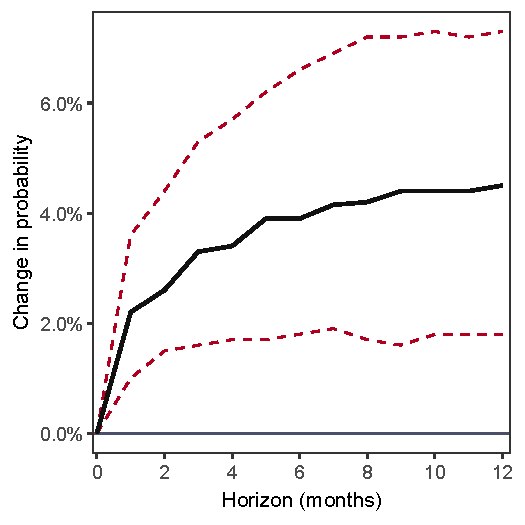
\includegraphics[width=\textwidth]{figures/tvar_switching_F_crisis.pdf}
    \caption{Reserve Flow Shock ($g^F$)}
    \label{fig:tvar_switch_F}
\end{subfigure}
\hfill
\begin{subfigure}[b]{0.32\textwidth}
    \centering
    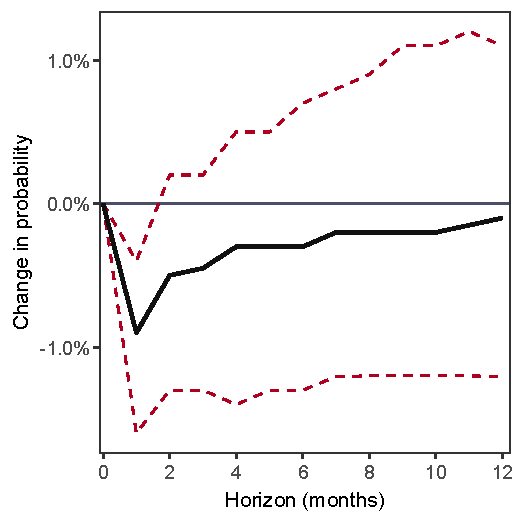
\includegraphics[width=\textwidth]{figures/tvar_switching_money_crisis.pdf}
    \caption{Base Money Shock ($g^H$)}
    \label{fig:tvar_switch_money}
\end{subfigure}
\hfill
\begin{subfigure}[b]{0.32\textwidth}
    \centering
    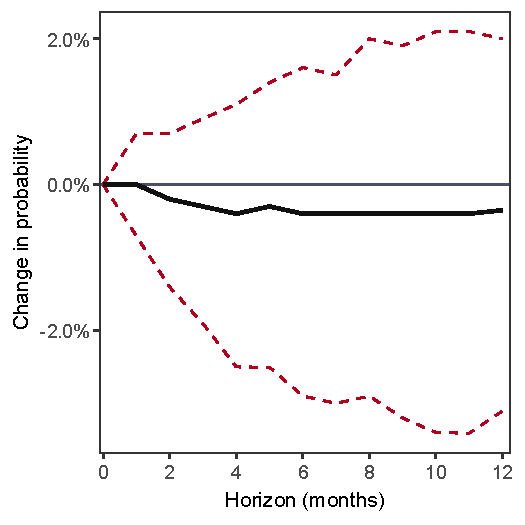
\includegraphics[width=\textwidth]{figures/tvar_switching_gold_crisis.pdf}
    \caption{World Gold Shock ($g^{gold}$)}
    \label{fig:tvar_switch_gold}
\end{subfigure}
\caption{Endogenous Regime Switching Probabilities from the Adverse Solvency-Growth State ($\Delta P(\Delta s_{t+h-1} \le \gamma)$)}
\label{fig:app_d04_switching}
\begin{minipage}{\textwidth}
    \vspace{0.3em}
    \footnotesize \textbf{Notes:} Simulated change in the probability of remaining in the adverse solvency-growth state ($\Delta s_{t-1} \le -4.615\%$, reflecting conditions of central-bank insolvency) following a one-standard-deviation structural innovation ($u_t$). Solid lines represent median bootstrap trajectories; dashed crimson lines denote 90\% empirical bootstrap confidence intervals ($B=500, R=1{,}000$). The horizontal line marks zero change in transition probability.
\end{minipage}
\end{figure}

The transition curves uncover two core empirical dynamics:
\begin{enumerate}[leftmargin=*,itemsep=1pt]
    \item \textbf{Buffer stock resilience in non-adverse times:} Starting from the non-adverse state, standard one-standard-deviation monthly shocks produce probability shifts near zero ($\Delta P \in [-0.4\%, +0.1\%]$). A transitory monthly disturbance cannot independently breach the $-4.615\%$ threshold. Entering the adverse solvency-growth state required the cumulative drainage of foreign exchange reserves over five consecutive quarters (late 1970 through late 1971). That exhaustion was driven by international credit line cancellations and import surges for capital equipment and food.
    \item \textbf{State persistence under adverse conditions:} Once the lagged Solvency Growth Gap enters the adverse state ($\Delta s_{t-1} \le -4.615\%$, reflecting conditions of central-bank insolvency), favorable commodity price shocks fail to reduce the simulated probability of remaining in that state ($\Delta P = -0.35\%$ at month 12, with confidence intervals spanning zero). In this dynamic simulation, the system exhibits substantial state persistence rather than rapid self-correction.
\end{enumerate}

\subsection{Secondary Structural Pathway Trajectories}
Figures~\ref{fig:app_d01_reserves}, \ref{fig:app_d02_imbalance}, and \ref{fig:app_d03_persistence} document the secondary transmission pathways in the Threshold VAR.

\begin{figure}[htbp]
\centering
\begin{subfigure}[b]{0.32\textwidth}
    \centering
    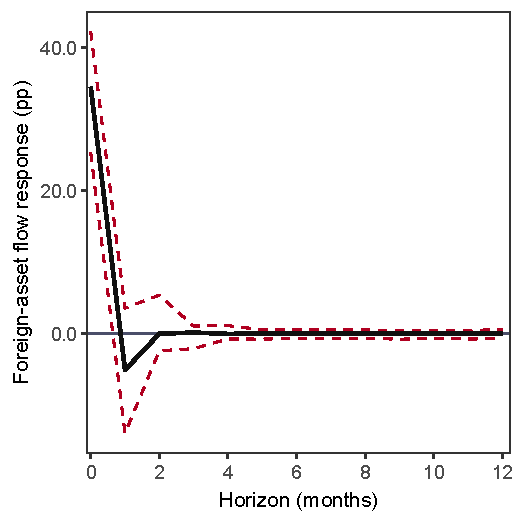
\includegraphics[width=\textwidth]{figures/tvar_girf_reserve_flow_insolv.pdf}
    \caption{Reserve Persistence ($g^F \to g^F$)}
    \label{fig:app_d_reserve_persistence}
\end{subfigure}
\hfill
\begin{subfigure}[b]{0.32\textwidth}
    \centering
    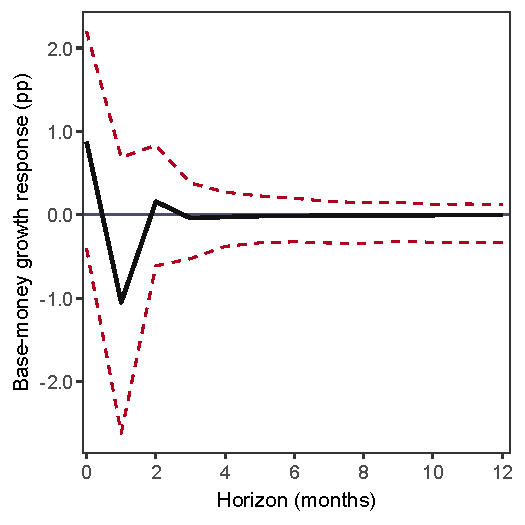
\includegraphics[width=\textwidth]{figures/tvar_girf_reserve_to_money_insolv.pdf}
    \caption{Reserve to Money ($g^F \to g^H$)}
    \label{fig:app_d_reserve_money}
\end{subfigure}
\hfill
\begin{subfigure}[b]{0.32\textwidth}
    \centering
    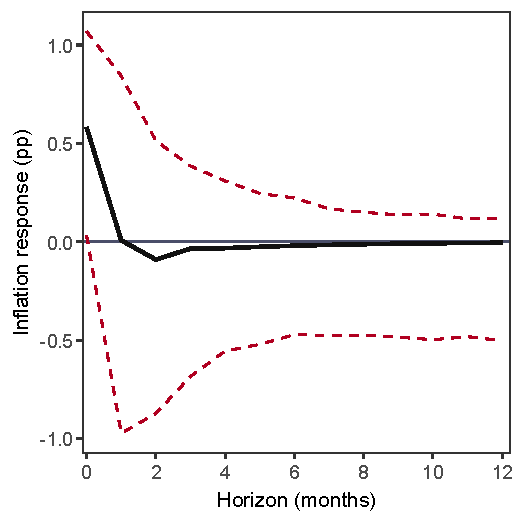
\includegraphics[width=\textwidth]{figures/tvar_girf_reserve_to_inflation_insolv.pdf}
    \caption{Reserve to Inflation ($g^F \to \pi_m$)}
    \label{fig:app_d_reserve_inflation}
\end{subfigure}
\caption{Dynamic GIRF Multipliers for Foreign Reserve Shocks in the Adverse Solvency-Growth State}
\label{fig:app_d01_reserves}
\begin{minipage}{\textwidth}
    \vspace{0.3em}
    \footnotesize \textbf{Notes:} Generalized Impulse Response Functions over a 12-month horizon in the adverse solvency-growth state ($\Delta s_{t-1} \le -4.615\%$, reflecting conditions of central-bank insolvency). Solid black lines represent median bootstrap responses to a one-standard-deviation reserve flow innovation; dashed crimson lines depict 90\% empirical bootstrap confidence intervals. The horizontal line marks zero.
\end{minipage}
\end{figure}

\begin{figure}[htbp]
\centering
\begin{subfigure}[b]{0.32\textwidth}
    \centering
    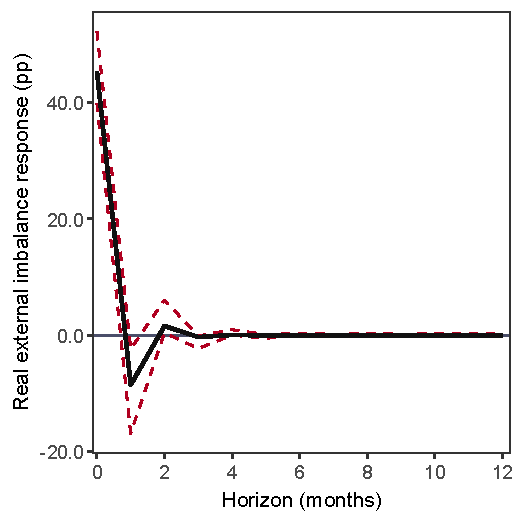
\includegraphics[width=\textwidth]{figures/tvar_girf_theta_persistence_insolv.pdf}
    \caption{Imbalance Persistence ($\Theta \to \Theta$)}
    \label{fig:app_d_theta_persistence}
\end{subfigure}
\hfill
\begin{subfigure}[b]{0.32\textwidth}
    \centering
    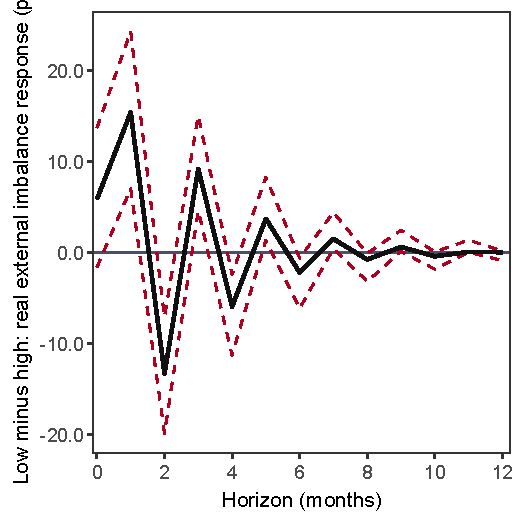
\includegraphics[width=\textwidth]{figures/tvar_girf_theta_difference.pdf}
    \caption{Regime Difference ($\Delta_{\Theta \to \Theta}$)}
    \label{fig:app_d_theta_diff}
\end{subfigure}
\hfill
\begin{subfigure}[b]{0.32\textwidth}
    \centering
    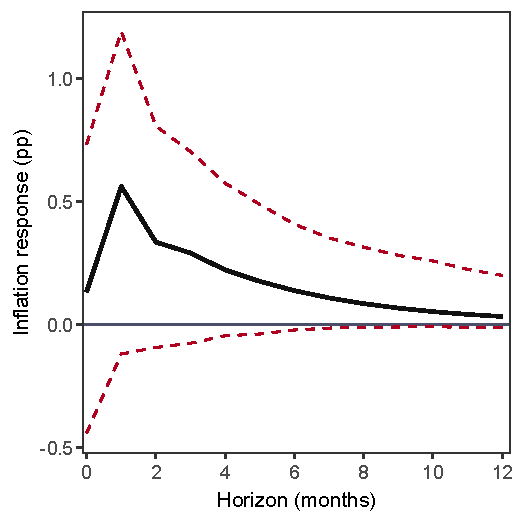
\includegraphics[width=\textwidth]{figures/tvar_girf_theta_to_inflation_insolv.pdf}
    \caption{Imbalance to Prices ($\Theta \to \pi_m$)}
    \label{fig:app_d_theta_inflation}
\end{subfigure}
\caption{Dynamic GIRF Multipliers for Real Structural Imbalance Shocks}
\label{fig:app_d02_imbalance}
\begin{minipage}{\textwidth}
    \vspace{0.3em}
    \footnotesize \textbf{Notes:} Generalized Impulse Response Functions over a 12-month horizon following a one-standard-deviation real structural trade imbalance shock ($\Delta\ln\Theta$). Solid black lines trace median bootstrap responses; dashed crimson lines denote 90\% empirical bootstrap confidence intervals.
\end{minipage}
\end{figure}

\begin{figure}[htbp]
\centering
\begin{subfigure}[b]{0.32\textwidth}
    \centering
    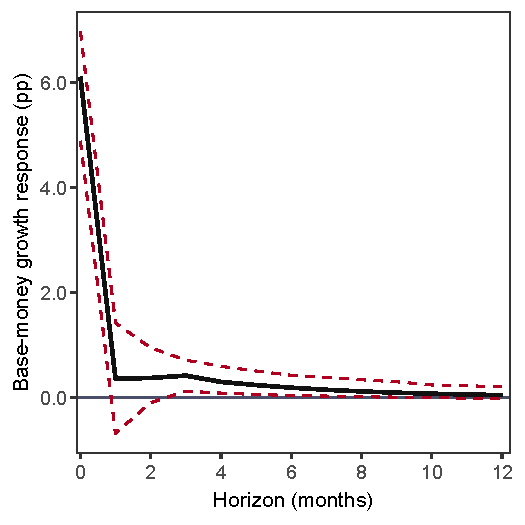
\includegraphics[width=\textwidth]{figures/tvar_girf_money_persistence_insolv.pdf}
    \caption{Money Persistence ($g^H \to g^H$)}
    \label{fig:app_d_money_persistence}
\end{subfigure}
\hfill
\begin{subfigure}[b]{0.32\textwidth}
    \centering
    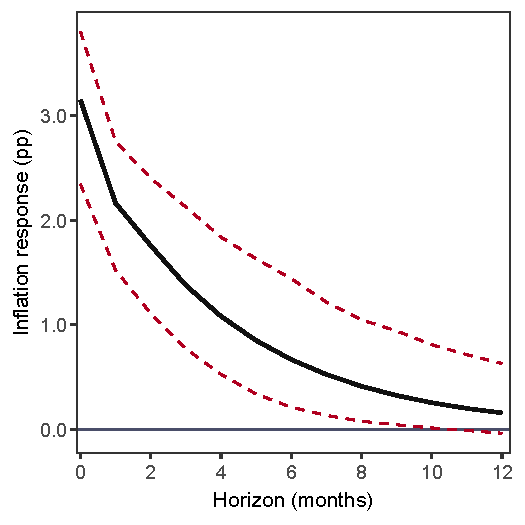
\includegraphics[width=\textwidth]{figures/tvar_girf_inflation_persistence_insolv.pdf}
    \caption{Inflation Persistence ($\pi_m \to \pi_m$)}
    \label{fig:app_d_inflation_persistence}
\end{subfigure}
\hfill
\begin{subfigure}[b]{0.32\textwidth}
    \centering
    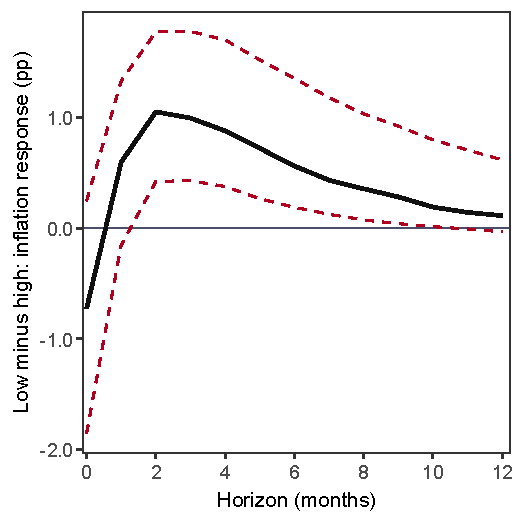
\includegraphics[width=\textwidth]{figures/tvar_girf_inflation_difference.pdf}
    \caption{Regime Difference ($\Delta_{\pi_m \to \pi_m}$)}
    \label{fig:app_d_inflation_diff}
\end{subfigure}
\caption{Dynamic GIRF Multipliers for Domestic Liquidity and Cost-Push Inertia}
\label{fig:app_d03_persistence}
\begin{minipage}{\textwidth}
    \vspace{0.3em}
    \footnotesize \textbf{Notes:} Generalized Impulse Response Functions over a 12-month horizon in the adverse solvency-growth state ($\Delta s_{t-1} \le -4.615\%$, reflecting conditions of central-bank insolvency). Solid black lines trace median bootstrap responses; dashed crimson lines denote 90\% empirical bootstrap confidence intervals.
\end{minipage}
\end{figure}

\subsection{Diagnostics for Block-Exogeneity and Structural Exclusion Restrictions}
Table~\ref{tab:app_d01_girf_differences} reports diagnostics for the nine block-exogenous and structurally excluded pathways:
\begin{enumerate}[leftmargin=*,itemsep=1pt]
    \item \textbf{World gold price exogeneity diagnostics:} Innovations to domestic international reserves ($g^F$), consumer price inflation ($\pi_m$), Central Bank base money ($g^H$), and the real trade gap ($\Delta\ln\Theta$) produce no statistically significant response in world gold prices across all 12 forecast horizons. Duration of significance is zero months throughout, with point estimates below $0.055$ percentage points. The data do not provide evidence against treating Chile as a price taker in international gold and hard-currency markets.
    \item \textbf{Structural trade imbalance exogeneity diagnostics:} Domestic nominal shocks to money and inflation produce no statistically significant response in the real structural trade imbalance ($\Delta\ln\Theta$). The trade gap was governed by external terms of trade and historical intermediate import requirements for copper mining equipment and industrial fuels.
    \item \textbf{Direct reserve and credit exclusions:} Imposing the restriction that the real trade gap ($\Delta\ln\Theta$) does not enter directly into contemporaneous reserve flow ($g^F$) or base money creation ($g^H$) equations results in exact impact neutrality ($h_0 = 0.000$). This restriction aligns with the directional Granger tests. Structural trade gaps operated sequentially through import bottlenecks and price adjustments ($\Delta\ln\Theta \to \pi_m$). The Central Bank then accommodated these price increases defensively ($\pi_m \to g^H$) to keep factories operating and workers paid.
\end{enumerate}

% Appendix E: Linear VAR Diagnostic Space and Auxiliary Specifications (EE1 Section 5.3)
% ==============================================================================
% Appendix E: Linear VAR Diagnostic Space and Auxiliary Specifications
% Preserves exploratory Systems 4, 5, and full-sample System 6
% ==============================================================================
\section{Linear VAR Diagnostic Space and Auxiliary Specifications}
\label{app:linear_var_diagnostics}

\subsection{Diagnostic Admissibility Criteria and Stopping Rule}
In accordance with the empirical discipline of this chapter, linear vector autoregressive models are admitted to the main text's inferential core only when they satisfy three baseline econometric criteria:
\begin{enumerate}
    \item \textbf{Modulus Stability (Criterion A):} All characteristic roots of the companion matrix lie strictly within the unit circle ($\max |\lambda_i| < 1$).
    \item \textbf{System Residual Whitening (Criterion B):} The multivariate Breusch--Godfrey Lagrange Multiplier test fails to reject the null of no residual autocorrelation at the 5\% level ($p > 0.05$).
    \item \textbf{Equation Residual Whitening (Criterion C):} Individual equation Breusch--Godfrey tests fail to reject the null of no autocorrelation at the 5\% level ($p > 0.05$) across all equations.
\end{enumerate}

During the exploratory empirical battery, three modular systems failed to satisfy these criteria: System 4 (Real Sector Dualism), System 5 (External Cost-Push), and the full-sample specification of System 6 (Central Bank Solvency). Rather than searching over ad-hoc lag specifications, non-linear trend adjustments, or arbitrary sub-samples until confirming the preferred theoretical hypotheses, the empirical audit sequence established a formal stopping rule. This appendix documents the diagnostic investigations across the lag search space ($k = 1, \dots, 12$), historical partitions (pre- and post-October 1973), and month-of-year seasonal controls, preserving the empirical record for full transparency.

\subsection{System 4: Real Sector Dualism (Descriptive Only)}
System 4 specifies the five-variable vector:
\begin{equation}
    Y^{(4)}_t = \begin{bmatrix} \pi_t & g_{H,t} & \Delta \ln \Theta_t & g_{\text{Manuf},t} & g_{\text{Mining},t} \end{bmatrix}',
\end{equation}
estimated over the full monthly sample (1960:01--1980:12, $N=250$). Table~\ref{tab:app_system4_real_dual} reports the exploratory Granger causality tests evaluated at the SBIC-selected lag ($k^*=2$).

\begin{table}[htbp]
\centering
\small
\renewcommand{\arraystretch}{0.90}
\caption{Exploratory Granger Tests: Real Sector Dualism ($N=250$, Full Sample)}
\label{tab:app_system4_real_dual}
\resizebox{\textwidth}{!}{%
\begin{tabular}{llcccc}
\toprule
\textbf{Dependent Variable} & \textbf{Predictor} & \textbf{Lag ($k^*$)} & \textbf{$F$-Statistic} & \textbf{$p$-value} & \textbf{$\sum \hat{\beta}_i$} \\
\midrule
Manufacturing Output ($g_{\text{Manuf},t}$) & Base Money Growth ($g_{H,t}$) & 2 & 3.636$^{**}$ & 0.0278 & $-0.333$ \\
Base Money Growth ($g_{H,t}$) & Manufacturing Output ($g_{\text{Manuf},t}$) & 2 & 2.306 & 0.1018 & $+0.046$ \\
Mining Output ($g_{\text{Mining},t}$) & Base Money Growth ($g_{H,t}$) & 2 & 0.908 & 0.4046 & $-0.096$ \\
Base Money Growth ($g_{H,t}$) & Mining Output ($g_{\text{Mining},t}$) & 2 & 0.654 & 0.5211 & $+0.022$ \\
Inflation ($\pi_t$) & Manufacturing Output ($g_{\text{Manuf},t}$) & 2 & 7.103$^{***}$ & 0.0010 & $-0.201$ \\
Manufacturing Output ($g_{\text{Manuf},t}$) & Structural Imbalance ($\Delta \ln \Theta_t$) & 2 & 1.526 & 0.2195 & $+0.076$ \\
\bottomrule
\end{tabular}%
}
\begin{minipage}{0.98\textwidth}
\vspace{0.3em}
\footnotesize \textbf{Notes:} Evaluated at $k^*=2$. Status: \textsc{Descriptive Only}. The system exhibits persistent residual autocorrelation (System Breusch--Godfrey $\chi^2 = 228.74, p < 0.0001$; minimum equation $p < 0.0001$). Residual autocorrelation persists when extending lags up to $k=12$, under historical calendar partitioning at October 1973, and with seasonal dummy controls. Accordingly, these statistics are not used for formal directional inference.
\end{minipage}
\end{table}

\subsection{System 5: External Cost-Push Transmission (Inconclusive)}
System 5 specifies the five-variable external transmission vector:
\begin{equation}
    Y^{(5)}_t = \begin{bmatrix} g_{P,\text{gold},t} & g_{e,t} & \Delta \ln \Theta_t & g_{H,t} & \pi_t \end{bmatrix}',
\end{equation}
estimated over 1960:01--1980:12 ($N=250$). Table~\ref{tab:app_system5_external} reports exploratory Granger tests at the SBIC-selected lag ($k^*=1$).

\begin{table}[htbp]
\centering
\small
\renewcommand{\arraystretch}{0.90}
\caption{Exploratory Granger Tests: External Cost-Push Transmission ($N=250$, Full Sample)}
\label{tab:app_system5_external}
\resizebox{\textwidth}{!}{%
\begin{tabular}{llcccc}
\toprule
\textbf{Dependent Variable} & \textbf{Predictor} & \textbf{Lag ($k^*$)} & \textbf{$F$-Statistic} & \textbf{$p$-value} & \textbf{$\sum \hat{\beta}_i$} \\
\midrule
World Gold Price ($g_{P,\text{gold},t}$) & Domestic Aggregates & 1 & \dots & $> 0.10$ & \dots \\
Inflation ($\pi_t$) & Structural Imbalance ($\Delta \ln \Theta_t$) & 1 & 5.113$^{**}$ & 0.0246 & $-0.019$ \\
Devaluation Rate ($g_{e,t}$) & Inflation ($\pi_t$) & 1 & 23.305$^{***}$ & $< 0.0001$ & $+0.689$ \\
Base Money Growth ($g_{H,t}$) & Devaluation Rate ($g_{e,t}$) & 1 & 17.037$^{***}$ & $< 0.0001$ & $+0.161$ \\
Inflation ($\pi_t$) & Devaluation Rate ($g_{e,t}$) & 1 & 1.697 & 0.1939 & $+0.046$ \\
\bottomrule
\end{tabular}%
}
\begin{minipage}{0.98\textwidth}
\vspace{0.3em}
\footnotesize \textbf{Notes:} Evaluated at $k^*=1$. Status: \textsc{Inconclusive}. The system exhibits persistent residual autocorrelation (System Breusch--Godfrey $\chi^2 = 310.16, p < 0.0001$; minimum equation $p < 0.0001$). Extending lag length to $k=12$, calendar partitioning, and seasonal controls fail to whiten the residuals. Furthermore, key relations display sensitivity to multivariate conditioning. These results are retained for documentation but not used for directional inference.
\end{minipage}
\end{table}

\subsection{System 6: Full-Sample Central Bank Solvency Diagnostics}
In the full sample (1960:01--1980:12, $N=250$), System 6 fails residual whitening across all tested lags $k \in \{1, 2, 3, 4\}$ (System Breusch--Godfrey $p < 0.0001$). However, partitioning the sample at October 1973 reveals that residual autocorrelation is concentrated in the post-1973 period under the crawling-peg regime. In the pre-October 1973 subperiod, residual autocorrelation is fully resolved at lag $k=3$ (System Breusch--Godfrey $p = 0.1262$; minimum equation $p = 0.0557$). As reported in Section~\ref{sec:granger_solvency_pre73} and Table~\ref{tab:core_granger_evidence}, System 6 is admitted to the main text strictly as a qualified, historically specific result for the pre-1973 era.

\end{appendices}


\end{document}
